% Options for packages loaded elsewhere
\PassOptionsToPackage{unicode}{hyperref}
\PassOptionsToPackage{hyphens}{url}
%
\documentclass[
]{article}
\usepackage{amsmath,amssymb}
\usepackage{iftex}
\ifPDFTeX
  \usepackage[T1]{fontenc}
  \usepackage[utf8]{inputenc}
  \usepackage{textcomp} % provide euro and other symbols
\else % if luatex or xetex
  \usepackage{unicode-math} % this also loads fontspec
  \defaultfontfeatures{Scale=MatchLowercase}
  \defaultfontfeatures[\rmfamily]{Ligatures=TeX,Scale=1}
\fi
\usepackage{lmodern}
\ifPDFTeX\else
  % xetex/luatex font selection
    \setmainfont[]{Times New Roman}
\fi
% Use upquote if available, for straight quotes in verbatim environments
\IfFileExists{upquote.sty}{\usepackage{upquote}}{}
\IfFileExists{microtype.sty}{% use microtype if available
  \usepackage[]{microtype}
  \UseMicrotypeSet[protrusion]{basicmath} % disable protrusion for tt fonts
}{}
\makeatletter
\@ifundefined{KOMAClassName}{% if non-KOMA class
  \IfFileExists{parskip.sty}{%
    \usepackage{parskip}
  }{% else
    \setlength{\parindent}{0pt}
    \setlength{\parskip}{6pt plus 2pt minus 1pt}}
}{% if KOMA class
  \KOMAoptions{parskip=half}}
\makeatother
\usepackage{xcolor}
\usepackage[top=3.5in,bottom=3.5in,left=3in,right=3in,margin=1in]{geometry}
\usepackage{longtable,booktabs,array}
\usepackage{calc} % for calculating minipage widths
% Correct order of tables after \paragraph or \subparagraph
\usepackage{etoolbox}
\makeatletter
\patchcmd\longtable{\par}{\if@noskipsec\mbox{}\fi\par}{}{}
\makeatother
% Allow footnotes in longtable head/foot
\IfFileExists{footnotehyper.sty}{\usepackage{footnotehyper}}{\usepackage{footnote}}
\makesavenoteenv{longtable}
\usepackage{graphicx}
\makeatletter
\def\maxwidth{\ifdim\Gin@nat@width>\linewidth\linewidth\else\Gin@nat@width\fi}
\def\maxheight{\ifdim\Gin@nat@height>\textheight\textheight\else\Gin@nat@height\fi}
\makeatother
% Scale images if necessary, so that they will not overflow the page
% margins by default, and it is still possible to overwrite the defaults
% using explicit options in \includegraphics[width, height, ...]{}
\setkeys{Gin}{width=\maxwidth,height=\maxheight,keepaspectratio}
% Set default figure placement to htbp
\makeatletter
\def\fps@figure{htbp}
\makeatother
\setlength{\emergencystretch}{3em} % prevent overfull lines
\providecommand{\tightlist}{%
  \setlength{\itemsep}{0pt}\setlength{\parskip}{0pt}}
\setcounter{secnumdepth}{5}
% definitions for citeproc citations
\NewDocumentCommand\citeproctext{}{}
\NewDocumentCommand\citeproc{mm}{%
  \begingroup\def\citeproctext{#2}\cite{#1}\endgroup}
\makeatletter
 % allow citations to break across lines
 \let\@cite@ofmt\@firstofone
 % avoid brackets around text for \cite:
 \def\@biblabel#1{}
 \def\@cite#1#2{{#1\if@tempswa , #2\fi}}
\makeatother
\newlength{\cslhangindent}
\setlength{\cslhangindent}{1.5em}
\newlength{\csllabelwidth}
\setlength{\csllabelwidth}{3em}
\newenvironment{CSLReferences}[2] % #1 hanging-indent, #2 entry-spacing
 {\begin{list}{}{%
  \setlength{\itemindent}{0pt}
  \setlength{\leftmargin}{0pt}
  \setlength{\parsep}{0pt}
  % turn on hanging indent if param 1 is 1
  \ifodd #1
   \setlength{\leftmargin}{\cslhangindent}
   \setlength{\itemindent}{-1\cslhangindent}
  \fi
  % set entry spacing
  \setlength{\itemsep}{#2\baselineskip}}}
 {\end{list}}
\usepackage{calc}
\newcommand{\CSLBlock}[1]{\hfill\break\parbox[t]{\linewidth}{\strut\ignorespaces#1\strut}}
\newcommand{\CSLLeftMargin}[1]{\parbox[t]{\csllabelwidth}{\strut#1\strut}}
\newcommand{\CSLRightInline}[1]{\parbox[t]{\linewidth - \csllabelwidth}{\strut#1\strut}}
\newcommand{\CSLIndent}[1]{\hspace{\cslhangindent}#1}
% 段落インデントと段落間の空白をAPA仕様に設定
\usepackage{indentfirst} 
\setlength{\parindent}{1.27cm} 
\setlength{\parskip}{0pt}      

% パッケージ
\usepackage{titlesec}
\usepackage{fancyhdr}
\usepackage{linguex}
\PassOptionsToPackage{table}{xcolor}
\usepackage{xcolor}
\usepackage{tabularx}


% セクションタイトルのフォーマット(APA第7版に準拠)

% Level 1: Section (Flush left, Bold, Large)
\titleformat{\section}[block]
  {\normalfont\bfseries\fontsize{26}{28}\selectfont}
  {\thesection}{1em}{}

\titlespacing*{\section}{0pt}{3.5ex plus 1ex minus .2ex}{2.3ex plus .2ex}

% Level 2: Subsection (Flush left, Bold)
\titleformat{\subsection}[block]
  {\normalfont\bfseries\fontsize{18}{22}\selectfont}
  {\thesubsection}{1em}{}

\titlespacing*{\subsection}{0pt}{3.0ex plus 1ex minus .2ex}{2.0ex plus .2ex}

% Level 3: Subsubsection (Flush left, Bold Italic)
\titleformat{\subsubsection}[block]
  {\normalfont\bfseries\itshape\fontsize{14}{16}\selectfont}
  {\thesubsubsection}{1em}{}

\titlespacing*{\subsubsection}{0pt}{2.5ex plus 1ex minus .2ex}{2.0ex plus .2ex}

% Level 4: Paragraph (Indented, Bold, run-in heading, ends with period)
\titleformat{\paragraph}[runin]
  {\normalfont\bfseries\normalsize}
  {\theparagraph}{1em}{}
  
\titlespacing*{\paragraph}{1.27cm}{3.0ex plus 1ex minus .2ex}{1em}

% Level 5: Subparagraph (Indented, Bold Italic, run-in heading, ends with period)
\titleformat{\subparagraph}[runin]
  {\normalfont\bfseries\itshape\normalsize}
  {\thesubparagraph}{1em}{}

\titlespacing*{\subparagraph}{1.27cm}{3.0ex plus 1ex minus .2ex}{1em}

% 標準文字サイズ設定(必要なら)
\renewcommand{\normalsize}{\fontsize{12}{16.5}\selectfont}

% fancyhdr設定
\usepackage{fancyhdr}
\pagestyle{fancy}
\fancyhf{}  
\fancyhead[L]{\nouppercase{\leftmark}}  
\fancyfoot[C]{\thepage} 

% セクションタイトルを leftmark に反映させる設定
\makeatletter
\renewcommand{\sectionmark}[1]{\markboth{\thesection\ #1}{}}
\makeatother
\usepackage{booktabs}
\usepackage{longtable}
\usepackage{array}
\usepackage{multirow}
\usepackage{wrapfig}
\usepackage{float}
\usepackage{colortbl}
\usepackage{pdflscape}
\usepackage{tabu}
\usepackage{threeparttable}
\usepackage{threeparttablex}
\usepackage[normalem]{ulem}
\usepackage{makecell}
\usepackage{xcolor}
\ifLuaTeX
  \usepackage{selnolig}  % disable illegal ligatures
\fi
\usepackage{bookmark}
\IfFileExists{xurl.sty}{\usepackage{xurl}}{} % add URL line breaks if available
\urlstyle{same}
\hypersetup{
  hidelinks,
  pdfcreator={LaTeX via pandoc}}

\author{}
\date{\vspace{-2.5em}}

\begin{document}

\begin{titlepage}
  \centering
  \vspace*{4cm}

  {\fontsize{24}{28}\selectfont \textbf{EFFECTS OF NUMBER DISSIMILARITY ON JAPANESE EFL LEARNERS' PROCESSING OF SUBJECT AND OBJECT RELATIVE CLAUSES}\par}
  \vspace{1.5cm}

  {\fontsize{16}{20}\selectfont
  A master’s thesis presented to the Faculty of \\
  English/Linguistics Studies of the University of Stuttgart \\
  for the degree of Master of Arts in English and \\
  American Studies/English Linguistics
  \par}
  \vspace{2cm}

  {\fontsize{16}{20}\selectfont Presented by: \\
  Takumi Kobayashi \par}
  \vspace{1cm}

  {\fontsize{16}{20}\selectfont Supervised by: \\
  Dr. Titus von der Malsburg \par}
  \vfill

  {\fontsize{14}{18}\selectfont Stuttgart, June 11, 2025 \par}
\end{titlepage}

\clearpage
\thispagestyle{empty}  
\pagenumbering{roman}  
\setcounter{page}{1}

\clearpage
\thispagestyle{plain}  
\pagenumbering{roman}  
\setcounter{page}{2}   
\section*{Acknowledgments}
\vspace*{1.5cm}

First of all, I am profoundly grateful to my parents and brother. I was
born and raised in a small town surrounded by mountains, like a
fortress, in Japan. Although it is a beautiful place, it is unbelievably
conservative at the same time. My parents, however, showered me with
unconditional love and gave me the courage to step out into the world.
From my mother, I received imagination about the ``outside world''; from
my father, courage and drive; and from my younger brother, peace of
mind.

I also sincerely thank my partner Sarah and her family. Their continuous
encouragement and devoted support during times when I was overwhelmed by
anxiety meant the world to me. Above all, I am thankful for meeting
Sarah and her family and always being by my side.

Most importantly, I wish to express my deepest gratitude to Dr.~Titus
von der Malsburg, my thesis supervisor. Although his methodological and
theoretical advice always gives me variable insights, his positivity,
smile and belief in my ability gently push me forward and give me
confidence that I could succeed. I would also like to thank Dr.~Anna
Pryslopska and Mr.~Nico Wildermuth for their valuable advice on the
experimental methods used in my master's thesis.

Special appreciation is also extended to the members of the department,
including the previous program coordinator of MA-EASEL, Dr.~Thomas
Waegenbaur for his patient support and guidance, and the ifLA secretary,
Mr.~Ralf Bothner for his flexible support.

\clearpage
\thispagestyle{plain}  
\section*{Abstract}
\vspace*{1.5cm}

\noindent This thesis investigates asymmetry in processing difficulty in
Japanese EFL learners between English subject and object relative
clauses. Besides exploring the existence of the asymmetry between the
two different types of relative clauses, the facilitation effect of
number dissimilarity on processing the relative clauses is also
examined. In other words, the first purpose of this thesis is to clarify
whether Japanese EFL learners exhibit the asymmetry (subject relative
clauses are easier to process than object relative clauses) which is
reported by a majority of the existing studies. The second goal is to
examine whether the EFL (English as a foreign language) learners utilize
number marking as a clue to process the relative clauses more smoothly
or accurately. To elucidate the presence of the asymmetry and the
facilitation effect of number dissimilarity, an online self-paced
reading task is conducted and reading time and comprehension accuracy
for the questions are analyzed. The findings of this thesis showed the
asymmetry of the processing difficulty, meaning Japanese EFL learners
read subject relative clauses faster than object relative clauses.
Another key finding is the Japanese EFL learners utilized the number
dissimilarity between the head and local NPs to process the sentences
with relative clauses. Since Japanese usually does not use overt marking
in number, the facilitation effect of the number mismatch in Japanese
EFL learners supports the learners of English as a foreign language can
sharpen the sensitivity toward numbers and make use of it as a hint to
process relative clauses. To the best knowledge of the author, this
thesis is the first study that focuses on the facilitation effect of
number dissimilarity in the Japanese EFL learners. In addition to that,
the studies focusing on the facilitation effects of morphological
marking to relative clause processing are still scarce. Therefore, this
study contributes to our understanding of the facilitation effects of
morphological marking on sentences with relative clauses. However, it is
indispensable to accumulate the studies with different methodologies,
participants and language settings to build a deeper understanding.

\clearpage
\pagenumbering{roman}
\setcounter{page}{4}

\pagestyle{plain}
\tableofcontents

\clearpage
\pagestyle{plain}
\listoffigures

\clearpage
\pagestyle{plain}
\listoftables

\clearpage
\pagenumbering{arabic}
\setcounter{page}{8}

\thispagestyle{empty}
\vspace*{-1cm}
\begin{flushleft}
\Huge \textbf{Chapter 1}
\end{flushleft}
\vspace{0.3cm}

\noindent

\rule{\linewidth}{0.6pt}

\pagestyle{fancy}
\fancyhf{}  
\fancyhead[L]{\nouppercase{\leftmark}}
\fancyfoot[C]{\thepage}

\section{Introduction}\label{introduction}

Figuring out how complex sentences are processed is meaningful for
psycholinguists to understand the mental processes underlying language
processing and comprehension (Gordon et al., 2001). In the field of
psycholinguistics, sentences with relative clauses (RCs) have been
frequently highlighted as a research subject over the decades due to
their nested and relatively complex structure. As it is explained more
deeply in the following section, a large body of existing studies have
supported the finding that subject relative clauses (SRCs) are easier to
process than object relative clauses (ORCs) (Gordon et al., 2001;
Traxler et al., 2002). This phenomenon, the subject-object asymmetry has
been studied by many scholars across different language settings and
methodologies. The subject-object asymmetry is positioned as the main
topic in the present study because there is still room for further
study, especially in the L2/EFL context.

There are striking differences in the morphosyntactic features of
relative clauses across languages. For example, in German relative
clauses, case marking is essential, whereas this feature is not observed
in English relative clauses. German speakers have been reported to rely
on these case distinctions as cues to facilitate processing of relative
clauses. Even children as young as 5--6 years old use case marking to
comprehend relative clauses correctly (Edeleva, 2023). In addition,
German and English have head-initial structure. However, some languages
such as Japanese or Korean have head-final structure. These
cross-linguistic differences in structures and morphological systems
play some roles in relative clause processing. The present study focuses
on the influence of cross-linguistic factors, particularly the influence
of Japanese as a first language on English RC processing.

Another perspective that this study examines is the influence of number
dis/agreement or number mis/matching on the RC processing. In some
languages such as English and German, nouns are morphologically marked
and distinguished based on whether they are singular or plural. However,
other languages such as Japanese do not mark nouns morphologically for
number, except in some specific cases. It is important to note that the
concepts of singularity and plurality exist when recognizing objects.
Japanese language does not consistently mark singular/plural
distinctions through inflection or morphological elements. Thus, it is
meaningful to examine whether this morphological marking or additional
elements would back up parsers to process sentences with RCs. In other
words, learners of second or foreign languages encounter number marking
as a new concept through learning the target language. For instance,
Japanese EFL learners usually encounter the number agreement and
morphological marking in English for the first time through the school
English class and native English speakers who start learning Japanese
experience the system not required number agreement. Needless to say,
there are many combinations of those language settings. In this study,
the influence of differences in number agreement between Japanese and
English is regarded as a possible factor which affects the Japanese EFL
learners' processing of relative clauses.

Studies investigating the processing of relative clauses began with a
focus on English as a first language, subsequently expanding to explore
the influences across a variety of other languages and cross-linguistic
contexts. Even though many previous studies have explored
cross-linguistic influence between different combinations of target
languages, the studies considering the effects of number mis/matching on
RC processing in EFL (English as a foreign language) are still scarce.
Therefore, the present study examines both relative clause processing
and influences of number mis/match between the head and local nouns in
the sentences with RCs as the two main topics

\subsection{Overview}\label{overview}

This thesis is structured as follows. In Chapter 2, the foundation of
relative clauses (RCs), including RC types, structures and
cross-linguistic differences are covered. Afterwards, the two central
topics of this thesis are recapped. First, the subject-object asymmetry,
which is a main topic of this thesis, is introduced along with various
accounts for this phenomenon. In fact, there are numerous accounts and
theories aiming to explain the mechanism of the subject-object asymmetry
from different viewpoints. This thesis attempts to overview those
different accounts by dividing the accounts into four types: syntactic
and typological accounts, memory-based accounts, experience-based
account, and semantic account. After presenting the overview of the
subject-object asymmetry and the possible accounts, another main theme
of this thesis, which is the influence of number morphology on relative
clause processing, is brought into focus. A theory called Relativized
Minimality (RM) underlying the hypothesis that the number morphology
helps parsers process relative clauses more easily and smoothly is
reviewed. Subsequently, some existing empirical studies that reported
the facilitation effects of the number dissimilarity on processing RCs
are introduced.

Chapter 3 outlines the research questions and corresponding hypotheses
of this thesis. There are two research questions. First, it is verified
whether Japanese EFL learners show the subject-object asymmetry when
reading English sentences with relative clauses. The second question is
whether the number dissimilarity between the head and local NPs
facilitates their processing of relative clauses. Since there are
several existing studies that have confirmed the asymmetry in Japanese
EFL learners, it is hypothesized that the participants in this study
would show the asymmetry as reported in those reference studies. In
regards to the second research question, there are no reference studies
with Japanese EFL learners to the best knowledge of the author.
Therefore, the hypothesis is based on contrasting results between
existing studies recruited participants with different first languages.
Based on the fact that there is no overt marking of numbers in Japanese
and the results from a study with Chinese EFL learners did not show a
facilitation effect, the hypothesis established there would be no
facilitation effect of the number mismatch on RC processing by Japanese
EFL learners.

Chapter 4 explains the methodology in order to probe the two research
questions. Besides the questionnaire about participants' general and
language-related background, the online self-paced reading task is
conducted. This section provides detailed information on the online
self-paced reading task with the information of participants, task,
stimuli, design and procedure.

In Chapter 5, the results of the online self-paced reading task and
statistical analysis towards the results are presented. At the beginning
of this section, it is explained how the collected data is pre-processed
and controlled in quality. After that the results of statistical
analyses are reported separately in comprehension accuracy and reading
time. In brief, the reading time shows some differences among conditions
and proves the existence of the subject-object asymmetry in Japanese EFL
learners. Contrary to the initial hypothesis regarding the second
research question, the facilitation effect of the number dissimilarity
is confirmed based on the reading time data. This particular result
provides new data from the previously untested participant group and
language setting.

In Chapter 6 and 7, it is discussed how this study interprets the
results from the self-paced reading task and pre-existing studies and
how the study can be improved in certain aspects. This study confirmed
both the subject-object asymmetry and the facilitation effect of the
number mismatch in relative clause processing by the Japanese EFL
learners. Those results support most existing studies reporting the
asymmetry and also provides new findings on the facilitation effects of
number mismatch in Japanese EFL learners. Indeed, these results are
novel in that they suggest that English learners, especially those whose
first language, Japanese does not mark number in general, utilize number
information as a cue when processing English relative clauses. However,
due to the absence of a control group of native English speakers and the
relatively small sample size, it is still premature to generalize the
findings of this study. In addition, there is still some room for
improvement in the experimental stimuli, particularly in terms of
semantic control. Overall, this thesis presents both strengths and areas
for further improvement.

\newpage

\clearpage
\thispagestyle{empty}  % ← 章扉ページはヘッダー・フッターなし
\vspace*{-1cm}
\begin{flushleft}
\Huge \textbf{Chapter 2}
\end{flushleft}
\vspace{0.3cm}
\noindent\rule{\linewidth}{0.6pt}
\pagestyle{fancy}  % ← 通常ページに戻る

\section{Background}\label{background}

\subsection{Relative Clauses}\label{relative-clauses}

\indent Relative clauses (RCs) are the clauses that modify nouns.
Relative clauses are frequently employed in many languages due to their
functionality.In English, there are some types of relative clauses based
on the grammatical and semantic roles of the head nouns. These different
types of relative clauses are overviewed in the following sub-section,
``Subject-Object Asymmetry and Various Accounts''. One of the focal
points in this thesis is the difference between subject relative clauses
(SRCs) and object relative clauses (ORCs). Referring to the example
sentences (1a-b), the relative clauses are bracketed. In the sentence
(1a), the head noun, \emph{the reporter} is interpreted as the subject
of the verb, \emph{attacked} in the relative clause, via a dependency
formed by the relative pronoun, \emph{that}. In other words, the main
clause subject, \emph{the reporter} also plays as the subject in the
relative clause. Conversely, the head, \emph{the reporter} is
interpreted as the object of the verb, \emph{attacked} in the relative
clause in the example sentence (1b). In the sentence (1b), the main
clause subject, \emph{the reporter} plays two different grammatical
roles in the main and relative clauses.

\vspace{1em}
{
\setlength{\parindent}{0pt}
\noindent
\begin{tabular}[t]{@{}ll}
(1a) The reporter \textbf{[that attacked the senator]} disliked the editor. [SRC] \\
(1b) The reporter \textbf{[that the senator attacked]} disliked the editor. [ORC] \\
\end{tabular}
\vspace{1em}

\noindent
\begin{quote}
\small
\textit{Note.} These examples are from Warren \& Gibson (2005, p.752).
\end{quote}
\vspace{1em}
}

It is beneficial to investigate the comprehension and production of
these two different relative clauses not only to see processing and
productive difficulty between SRCs and ORCs, but also to explore the
mechanism of language processing including the different memory load and
processing strategies. It contributes to building and reflecting the
morphosyntactic and semantic theories, and to visualize the
cross-linguistic difference and construct implicational universals over
languages.

In addition to the different types of RCs based on the grammatical and
semantic roles of the head noun of the relative clauses, there are also
cross-linguistic differences in terms of structures and use of relative
clauses. First, different languages adopt the different orders of
constituents of relative clauses. Some languages employ head-initial
structure and others contain head-final structure of relative clauses.
In other words, the head-initial structure has the word order like the
head noun is deployed first then the relative clause follows after the
head noun. On the other hand, the relative clause comes first and then
the head noun follows in the head-final structure. Interestingly, there
are tendencies which languages have which structural types as explained
as follows by Kortmann (2020).

\vspace{1em}

\begin{quote}
One hallmark of typology is its constant effort to establish
correlations between properties of different languages. For example, in
most languages where the verb precedes the object (so-called
VO-languages like English or French), prepositions and relative clauses
follow their nominal heads. Conversely, most OV-languages (like Turkish
and Japanese) have postpositions and relative clauses which precede
their nominal heads. Such generalizations are preferably formulated as
so-called implicational universals, e.g., ``A language which has SOV as
its canonical word order is very likely to have postpositions.''

--- Kortmann (2020, p.117)
\end{quote}

\vspace{1em}

Yet it is not merely a cross-linguistic difference, positions of
subordinate clauses are also considered influential to the processing
difficulty. The place of the subordinate clauses are categorized
left-embedded, center-embedded, and right-embedded as in the example
sentences (2a-c) below. In English, the center-embedded relative clauses
have been reported as the hardest of all to process because of their
structure like a hamburger. Parsers read a part of the main clause
first, then delve into the relative clause, and they finally come back
to the main clause again after reading the whole relative clause. On the
other hand, sentences with right and left-embedded clauses can be halved
between the main and subordinate clauses. Actually, there are some
studies compared processing difficulties among these different embedding
positions. Zhai et al.~(2019) conducted the eye-tracking experiment with
manipulated sentences with center-embedded, left-embedded, and
right-embedded reduced relative clauses. As a result, the Chinese EFL
learners showed center-embedded relative clauses to the hardest,
followed by right-embedded, and the left-embedded as the easiest. By
confirming the eye movement measures, it was reported that the
participants had more frequent fixations and also longer fixation
duration especially at the part of center-embedded relative clauses, and
also the parsers showed more complicated scanning pattern which implies
the center-embedded relative clauses induced confusion in Chinese EFL
learners during their processing of relative clauses in English.
Furthermore, the difficulty of the center-embedded relative clauses has
been reported in other studies as well (Hashimoto \& Hirai, 2007).

\vspace{1em}

\setlength{\parindent}{0pt}
\noindent
\begin{tabular}[t]{@{}p{0.05\linewidth} p{0.75\linewidth} >{\raggedleft\arraybackslash}p{2.5cm}@{}}
(2a) & The cheese \textbf{[the rat [the cat chased] ate]} was rotten. & {\small [center-embedded]} \\
(2b) & The cat chased the rat \textbf{[that ate the cheese [that was rotten]]}. & {\small [right-embedded]} \\
(2c) & \textbf{[[[John]'s brother]'s wife]'s friend} came to see me. & {\small [left-embedded]} \\
\end{tabular}

\vspace{0.5em}

\noindent
\begin{quote}
\small
\textit{Note.} These examples are from Kuno (1974, p.119).
\end{quote}

\vspace{1em}

\setlength{\parindent}{1.27cm}

In addition to the word order, relative clauses in some languages
explicitly use relative pronouns like, ``that'' or ``which'' in English.
However, languages like Japanese and Korean use no relative pronouns. If
the languages have agreements including number, case and gender, the
relative pronouns also visibly mark those features like in German. In
English, relative pronouns are omitted from relative clauses under
certain conditions and informal spoken situation. As for a further
difference, restrictive relative clauses (also known as defining
relative clauses) and non-restrictive relative clauses (also called as
non-defining relative clauses) are separated with comma for
non-restrictive relative clauses in English. The restrictive relative
clauses explain the essential information about the head and the
non-restrictive relative clauses explain supplemental information about
the head noun. Languages like Japanese does not explicitly mark the
distinction between restrictive and non-restrictive relative clauses and
these two different RC types are inferred from context and prosody. In
German, both restrictive and non-restrictive relative clauses tend to be
marked with comma, which also differs from English and Japanese. When
listing those differences in word order and explicit marking of relative
clauses among different languages, the list could be endless.
Nevertheless, such cross-linguistic variations are frequently studied in
the context of multilingualism and second or foreign language studies.
These studies help reveal how speakers' first languages influence the
processing and production of relative clauses in their second or foreign
languages. Some of the existing empirical studies focused on those
cross-linguistic differences are introduced in the following
sub-section.

\indent As introduced above, relative clauses vary widely across
languages in their structure, marking, and usage. Also, relative clauses
are categorized based on the grammatical and semantic roles of the head
noun into subject relative clauses, object relative clauses and so on.
Among the various types of RCs, subject relative clauses (SRCs) and
object relative clauses (ORCs) have received particular attention in the
psycholinguistic field. This is primarily due to the robust asymmetries
observed in their processing and acquisition patterns across many
languages. The asymmetry between SRCs and ORCs is one of the fundamental
topics in this thesis. The next section describes the phenomenon of
SRC--ORC asymmetry and reviews key theoretical accounts for the
asymmetry.

\subsection{Subject-Object Asymmetry and Various
Accounts}\label{subject-object-asymmetry-and-various-accounts}

\indent A large body of previous studies has reported that subject
relative clauses (SRCs) are easier than object relative clauses (ORCs)
to process in various languages based on empirical data from
eye-tracking or online self-paced reading experiments (e.g., Staub,
2010; Mak et al., 2006; Cohen \& Mehler, 1996; Schriefers et al., 1995;
Kwon et al., 2010; Ishizuka et al., 2003). As explored in the previous
section, there exist different types of relative clauses within and
across languages. Despite that, most studies have confirmed the
existence of the subject-object asymmetry. On the other hand, there are
actually studies reporting the opposite asymmetry that ORCs are easier
than SRCs, for instance in Chinese (Gibson \& Wu, 2013), Hebrew (Arnon,
2010) and Basque (Carreiras et al., 2010). Currently more studies have
supported the existence of the asymmetry between SRCs and ORCs although
there are some cases reporting the contrary results. It is also an
undeniable fact that those supporting studies have been conducted
majorly in European languages such as English, German, and Dutch. In
other words, the studies examining the asymmetry in non-European
languages and also studies in the second language or foreign language
contexts still remain limited. While many researchers generally agree
that subject relative clauses (SRCs) are easier to process than object
relative clauses (ORCs) across languages, the situation with less
studies with non-European languages suggest that the widely accepted
view might shift in the future, depending on the accumulation of more
empirical data from understudied languages.

The widely observed processing advantage of subject relative clauses
(SRCs) over object relative clauses (ORCs) has attracted significant
attention in the field of psycholinguistics. Numerous experimental
studies, especially those using eye-tracking, self-paced reading, and
ERP methodologies, have consistently shown that SRCs are read more
quickly and comprehended more easily than their ORC counterparts. This
asymmetry has prompted researchers to propose various theoretical
accounts that endeavor to explain the cognitive and structural
underpinnings of this phenomenon. Referring to the example (3a-b), the
word order from the subject of the main clause to the end of the
relative clause in sentence (3a) with omitting the relative pronoun,
\emph{that} follows SVO order. This order is canonical in English. On
the other hand, the sentence (3b) starting from the subject of the main
clause then after the subject of the relative clause appears immediately
which is confusing to parsers as of the order like SSV order (Warren \&
Gibson, 2005). Others argue that SRCs place a lower burden on working
memory because the parsers are demanded to hold the information of the
head NP longer till attaching it to the main clause verb in ORC
sentences (King \& Just, 1991).

Apart from the syntactic structure and memory load based on the linear
distance, some studies focus on the frequency of the RC types and words
used in the sentences with relative clauses. Simply put, their view is
that more frequent and familiar structures and lexical combinations
should be read faster and more accurately because parsers get used to
them and rather expect those canonical patterns are coming. Semantic and
discourse factors have also been studied recently and it has been
reported that semantic factors also play a role in shaping how different
types of relative clauses are processed. Here the semantic relatedness
between the NP1 (head) and NP2 (local), thematic roles, animacy,
plausibility between the subject and verb and so on. In order to explore
these possibilities in greater depth, the following sections introduce
four major accounts that have been proposed in the literature: syntactic
or typological accounts, memory-based accounts, experience-based
accounts, and semantic accounts. All in all, these hypotheses offer
complementary insights into the mechanisms that may contribute to the
SRC advantage and help explain both cross-linguistic consistency and
variation.

\vspace*{1em}

\setlength{\parindent}{0pt}
\noindent
\begin{tabular}[t]{@{}p{0.05\linewidth} p{0.75\linewidth} >{\raggedleft\arraybackslash}p{0.15\linewidth}@{}}
(3a) & The reporter \textbf{[that attacked the senator]} disliked the editor. & [SRC] \\
(3b) & The reporter \textbf{[that the senator attacked]} disliked the editor. & [ORC] \\
\end{tabular}

\vspace*{0.5em}

\noindent
\begin{quote}
\small
\textit{Note.} These examples are from Warren \& Gibson (2005, p.752).
\end{quote}

\vspace*{1em}

\clearpage

\setlength{\parindent}{1.27cm}

\subsubsection{Syntactic Accounts}\label{syntactic-accounts}

The first group of the accounts is based on syntactic structure and
typological studies. In the following sub-sections, four different
typological and syntactic hypotheses which initially classified
different RC types and comparatively considered the processing
difficulty of those different RC types are introduced.The four major
hypotheses introduced here are grounded under differing theoretical
assumptions. Most of them are supportive toward the existence of the
subject-object asymmetry.

\paragraph{Noun Phrase Accessibility Hypothesis
(NPAH)}\label{noun-phrase-accessibility-hypothesis-npah}

One of the most influential syntactic accounts proposed to explain the
relative ease or difficulty in processing different types of relative
clauses is Noun Phrase Accessibility Hierarchy Hypothesis (NPAH)
introduced by Comrie and Keenan (1979). Although the original aim was to
clarify the typological constraints on relativization across languages
and not specifically to solve the processing asymmetry between SRCs and
ORCs, this hypothesis is based on implicational universals. In short,
Comrie and Keenan (1979) compared over 50 languages and suggested the
order in which grammatical roles are more or less frequently and
naturally relativized. Specifically, NPAH ranked grammatical roles such
as subject, direct object, indirect object, oblique, genitive, and
object of comparison---according to their accessibility to
relativization. As shown in Table 1, the order is as follows: subject
(SU) \textgreater{} direct object (DO) \textgreater{} indirect object
(IO) \textgreater{} oblique object (OBL, or object of preposition in
English: OPREP) \textgreater{} genitive (GEN) \textgreater{} object of
comparison (OCOMP). This order shows the universal hierarchy among those
different types. In other words, NPAH claimed that if a language has GEN
type of RCs, the language must have the rest in the higher hierarchy
(SU, DO, IO, and OPREP). It is also impossible to reverse and skip the
order in NPAH. For instance, it is unexpected that a language has GEN
type but no SU type. As introduced above, the main purpose of NPAH was
not to point out the mechanism of the subject-object asymmetry, rather
it offered significant insights from both educational and
psycholinguistic perspectives. Today, the NPAH is regarded as supporting
the view point that SRCs are more difficult than ORCs to process.

\vspace{1em}
\begin{table}
\centering
\caption{\label{tab:Table1_NPAH}Example sentences for different RC types in the NPAH (Gao, 2014)}
\centering
\begin{tabular}[t]{ll}
\toprule
RC type & Example\\
\midrule
SU (Subject) & the girl that came...\\
DO (Direct Object) & the girl that John hit...\\
IO (Indirect Object) & the girl that he spoke to...\\
OPREP (Object of Preposition) & the girl that he sat near...\\
GEN (Genitive) & the girl whose father died...\\
\addlinespace
OCOMP (Object of Comparative) & the girl that he is taller than...\\
\bottomrule
\end{tabular}
\end{table}
\vspace{1em}

\paragraph{Parallel Function Hypothesis
(PFH)}\label{parallel-function-hypothesis-pfh}

While the Noun Phrase Accessibility Hierarchy (NPAH) classified RC types
based on their grammatical functions, other studies have employed
classifications with other perspectives such as the linear order of
constituents and the syntactic position where the relative clause is
embedded within the sentence. According to Savin and Perchonock (1965,
as reported in Bever, 1970), the case which the first-encountering verb
in the sentence was the verb of the relative clause was harder to
comprehend than the pattern that the first-encountering verb was the
verb of the main clause. Combining with the example sentences (4a-b),
sentence (4a) is inferred harder than sentence (4b). Following the
hypothesis by Savin and Perchonock (1965), Bever (1970) considered that
listeners who participated in the listening task conducted by Savin and
Perchonock (1965, as reported in Bever, 1970) responded to the first
Noun-Verb (N-V) sequence which appeared in the sentence. In short, the
participants contained the bias as if the first N-V structure
constituted the main sentence structure (main clause). Yet this tendency
with expectation is based on canonical order and experience, this would
make confusion in specific cases such as the relative clauses. Since the
first verb in the sentence is expected to be the main clause verb, the
relative clauses, specifically center-embedded relative clauses would
cause confusion in listeners and parsers and they will be required for
reanalysis.

\vspace{1em}

\setlength{\parindent}{0pt}
\noindent
\begin{tabular}[t]{@{}p{0.06\linewidth} p{0.67\linewidth} >{\raggedleft\arraybackslash}p{0.22\linewidth}@{}}
(4a) & The boy \textbf{[who likes the girl]} hit the man. & {\small [first verb = RC verb]} \\
(4b) & The boy hit the man \textbf{[who likes the girl]}. & {\small [first verb = MC verb]} \\
\end{tabular}

\vspace{0.5em}

\noindent
\begin{quote}
\small
\textit{Note.} These examples are originally from Savin and Perchonock (1965) as cited in Bever (1970, p.295).
\end{quote}

\vspace{1em}

Related to the N-V sequence and order of constituents proposed by Bever
(1970), Sheldon (1974) illustrated the influence of the order and
relation between subject and object in both main and relative clauses.
Four different types of sentences (see Table 2) were designed and used
in the experimental task to examine three possible influential factors
on RC processing; the position of the embedded RC, word order in RC,
grammatical roles of the identical nouns. In the experiment, children of
native speakers of English participated in a toy-based comprehension
task. They used toy animals to demonstrate the meaning of sentences with
relative clauses. As a result, Sheldon (1974) reported that children
performed better under the condition where the co-referential NPs had
the same grammatical function such as both NP1 and NP2 had subject roles
and both NP1 and NP2 had object roles than the condition where the two
NPs had different grammatical roles such as NP1: subject and NP2: object
and NP1: object and NP2: subject. Based on Table 2, SS and OO which have
parallel functions eased children's comprehension. From the perspective
of the subject-object asymmetry, SS and OS are categorized as SRCs and
SO and OO are equivalent to ORCs. Therefore, the order of processing
difficulty proposed in Sheldon (1974) was not perfectly in accordance
with the subject-object relative asymmetry.

\clearpage

\vspace{1em}
\begingroup\fontsize{11}{13}\selectfont

\begin{longtable}[t]{llll}
\caption{\label{tab:Table2_Sheldon}Four RC Types Tested in Sheldon (1974)}\\
\toprule
Head\_NP & Local\_NP & Label & Example\\
\midrule
subject & subject & SS (parallel) & The dog that jumps over the pig bumps into the lion.\\
subject & object & SO (nonparallel) & The lion that the horse bumps into jumps over the giraffe.\\
object & subject & OS (nonparallel) & The pig bumps into the horse that jumps over the giraffe.\\
object & object & OO (parallel) & The dog stands on the horse that the giraffe jumps over.\\
\bottomrule
\end{longtable}
\endgroup{}
\vspace{1em}

\paragraph{Perceptual Difficulty Hypothesis
(PDH)}\label{perceptual-difficulty-hypothesis-pdh}

In 1970-1980s, the typological observations including the NPAH were
actively conducted by scholars. There are eventually some other
hypotheses proposing different hierarchical order of relative clause
types. As reviewed in above, the NPAH and the PFH also suggested
different hierarchies of processing difficulty. Considering from the
subject-object asymmetry, these orders are contrary. In addition to
these hypotheses, there is another hypothesis, Perceptual Difficulty
Hypothesis (PDH) which was proposed by Kuno (1974). Kuno (1974)
considered the effect of the short-term memory limitations on RC
processing and suggested a different order from the NPAH. The
perspective of PDH was more into processing difficulty, perceptual and
memory load. In the PDH, relative clauses were categorized into four
types (SS, SO, OS, and OO) the same as Sheldon (1974) based on the
grammatical role of the NPs in main and relative clauses (see Table 2).
The PDH described that the embedded positions of relative clauses affect
processing and acquisition difficulty. The center-embedded RCs were
reported as the hardest and right-embedded RCs (left-embedded RCs in
some languages) were regarded as easier (5a-c). Based on Kuno's
hypothesis, Hayashi (2019) contemplated that SS and SO which are
embedded in the central of the sentence, are supposed to be perceived
harder to process than OS and OO that are embedded on the right side of
the sentence in English. Thus, the PDH can be regarded as supporting the
subject-object asymmetry in relative clause processing. Generally
speaking, reading processing is conducted sequentially based on the
order of words coming to one's brain although speakers can guess which
contents or words are coming next by activating background knowledge and
canonical order. Speakers cannot memorize and retain all the words and
information in the cases that the sentences are long and complex.
Center-embedded relative clauses require listeners or readers to hold
the information longer and thus they reduce the comprehensibility.

\vspace{1em}

\setlength{\parindent}{0pt}
\noindent
\begin{tabular}[t]{@{}p{0.05\linewidth} p{0.75\linewidth} >{\raggedleft\arraybackslash}p{2.5cm}@{}}
(5a) & The cheese \textbf{[the rat [the cat chased] ate]} was rotten. & {\small [center-embedded]} \\
(5b) & The cat chased the rat \textbf{[that ate the cheese [that was rotten]]}. & {\small [right-embedded]} \\
(5c) & \textbf{[[[John]'s brother]'s wife]'s friend} came to see me. & {\small [left-embedded]} \\
\end{tabular}

\vspace{0.5em}

\noindent
\begin{quote}
\small
\textit{Note.} These examples are from Kuno (1974, p.119).
\end{quote}

\vspace{1em}

\clearpage

\paragraph{Subject-Object Hierarchy Hypothesis
(SOHH)}\label{subject-object-hierarchy-hypothesis-sohh}

\setlength{\parindent}{1.27cm}

The Subject-Object Hierarchy Hypothesis (SOHH), notably discussed and
proposed by Hamilton (1994), proposed an implicational grammatical
hierarchy among different types of relative clauses (RCs), based on
their syntactic structure and the processing loads they impose on
parsers. Unlike other hypotheses introduced earlier such as the Noun
Phrase Accessibility Hierarchy (NPAH), the Perceptual Difficulty
Hypothesis (PDH), or the Parallel Function Hypothesis (PFH), which focus
on typological, perceptual, or functional factors, SOHH emphasized
syntactic discontinuity or the structural disruption caused by embedding
a relative clause within a sentence. From the perspective of Hamilton,
discontinuity refers to the linear and hierarchical separation between
the head noun and its grammatical role within the relative clause, which
can increase memory load and make integration more difficult during
comprehension. Based on empirical data from sentence processing studies,
Hamilton (1994) proposed the following implicational hierarchy of
processing difficulty with the four RC types which were also used in
Parallel Function Hypothesis (PFH) and Perceptual Difficulty Hypothesis
(PDH).

\vspace{1em}

\(\text{OS} > \text{OO} \quad / \quad \text{SS} > \text{SO}\)

\textit{Note.} Here, the symbol ``\(>\)'' is interpreted as ``is easier
than and/or means as difficult as.''

\vspace{1em}

In this hierarchy, OS (Object-Subject) relative clauses are considered
the easiest to process, followed by OO (Object-Object) and SS
(Subject-Subject), with SO (Subject-Object). The most difficult pattern
is SO (Subject-Object). The rationale is that SO structures involve a
crossing of grammatical roles, which the subject of the main clause
functions as the object of the relative clause, leading to greater
syntactic complexity and a higher working memory load.

\vspace{1em}

\setlength{\parindent}{0pt}
\noindent
\begin{tabular}[t]{@{}p{0.05\linewidth} p{0.75\linewidth} >{\raggedleft\arraybackslash}p{2.5cm}@{}}
(6a) & They saw the boy who entered the room. & [OS] \\
(6b) & A man bought the clock that the woman wanted. & [OO] \\
(6c) & The man who needed a job helped the woman. & [SS] \\
(6d) & The dog that the woman owns bit the cat. & [SO] \\
\end{tabular}

\vspace{0.5em}

\noindent
\begin{quote}
\small
\textit{Note.} These examples are from Hamilton (1994, p.134).
\end{quote}

\vspace{1em}

\paragraph{Summary}\label{summary}

In this sub-section, the four different hypotheses suggesting the
hierarchy or order of processing and acquisition difficulty of differing
RC types. Overall, the NPAH and the PDH can be considered as backing up
the subject-object asymmetry, but SOHH and PFH are not in line with the
subject-object asymmetry. While those four hypotheses had different
viewpoints to approach aligning RC types, mostly the syntactic
structures such as order of constituent and grammatical roles of the NPs
in main and relative clauses were focused. Exploring the processing and
acquisition hierarchies of those different RC types has been actively
conducted since 1970s. In fact, many studies have attempted to verify
those major hypotheses in different languages and participant groups by
using different methodology. The summary of some of those verification
or related studies are listed and summarized in Appendix A. A noticeable
trend in the literature is that the NPAH has been examined more widely
and frequently than other hypotheses such as the PDH, the PFH, the SOHH.
Therefore the summary seems supporting NPAH strongly. This tendency can
be attributed to several factors such as theoretical influence,
methodological simplicity, and pedagogical relevance. Since NPAH is
deeply rooted in typological linguistics and associated with
implicational universals. The focal point is to draw the grammatical
accessibility of noun phrase positions across languages. Thereby, this
hypothesis would be relatively readily to apply for further typological
studies and studying cross-linguistic influences. NPAH can be verified
more simply under different languages, participants and methodological
settings. There is the suggested hierarchical order of RC types and
those can be smoothly applied to the experimental tasks. Unlike the
NPAH, other hypotheses requires psycholinguistic background and more
variables and possible influential factors. For instance,
psycholinguistic-orientated experimental methodologies (e.g., online
self-paced reading tasks and eye-tracking experiments) would generally
be required to verify the PDH in order to collect reaction or reading
time and to see the relation between RC types and working memory
constraints. To conduct some follow-up studies of the PFH and the SOHH,
the experimental design would require more sensitive controls of target
sentences due to additional factors such as match/mismatch condition of
grammatical roles between main and relative clauses.

\setlength{\parindent}{1.27cm}

\subsubsection{Memory-based Accounts}\label{memory-based-accounts}

After the major hypotheses that stemmed from syntactic views had been
actively studied around 1970-1980s, the targeted point shifted to the
relation between working memory or short-term memory constraints and
processing of relative clauses. In this sub-section, the relevant
studies that probed the association between working memory and
processing of different types of RCs are outlined. Likewise the
syntactic accounts, memory accounts have been continuously studied since
1990s-2000s. First, the background how the existing studies quantified
the working memory load during reading RC sentences is introduced. After
that, some empirical studies and their results are described by dividing
them into two genres: studies defined on working memory span as
individual difference and studies manipulated the target sentences and
tried to lead more general tendencies and association between memory
load and relative clause types.

\paragraph{Dependency Locality Theory
(DLT)}\label{dependency-locality-theory-dlt}

As introduced earlier, Kuno (1974) proposed Perceptual Difficulty
Hypothesis (PDH) from the perspective of relation between the working
memory constraints and different RC types, typically left, right and
center-embedded relative clauses. The implication suggested that the
center-embedded relative clauses are the hardest because the parsers are
required to hold the incomplete information of dependency between
subject and verb in the matrix or main clause while processing the
inserted relative clause. This implication stemmed from the syntactic
linear distance. Here the question is how to measure the processing
difficulty and memory load of different relative clauses.

Gibson (2000) quantified the costs of processing difficulty of nested
sentences and advocated Dependency Locality Theory (DLT). The DLT
attempted to calculate the processing difficultly of the sentences,
especially assuming the real-time or accumulating sentence processing.
In the DLT, the cost of difficulty was considered based on two
computational resources by simulating the real-time processing. The
first resource is for integration: connecting words into the structure
based on the processed information by the time. The second resource is
for storage: keeping the structure in memory and holding incomplete
dependencies. The DLT supported that SRC sentences are easier than ORC
sentences by numerically calculating the memory loads. Also, this
numerical system deepened the discussion of the relation between memory
load and RC processing.

The first computational cost is integration. Integration here is the
process that parsers connect the information from the part they have
already read by the time and delineate the sentence structure, solve the
dependencies and construct the meaning of the sentence. As for the
integration costs, two different processes of integration were
introduced in Gibson (2000): structural integration and discourse
integration. The structural integration is about how to fit the newly
coming element into the pre-existing incomplete structure. Referring to
the example sentences (7a-c) below, the verb of the main clause,
\emph{was} should be integrated with the subject of the main clause,
\emph{the writing}. However, there are some intervening elements between
these two words. In the structural integration, it is considered that
the longer distance between these two elements that are supposed be
attached, the more cost increases. Gibson (2000) suggested Energy Unit
(EU) to visualize the cost due to the amount length of intervening
elements. Simply put, EU is calculated by first designating the head of
the dependency, then counting intervening elements between the two
elements which are supposed to be attached including the subject and
verb of the matrix clause. In comparison between the sentence (7a) and
(7b), there is no intervening elements between the subject of the
sentence, \emph{the writing} and the verb of the sentence, \emph{was},
therefore, EU becomes 0 in the sentence (7a). On the other hand, there
are some intervening words between the subject and the verb of the main
clause in (7b). Counting the content words, EU becomes 3 (that, the
student, and submitted) in the sentence (7b).

Besides the structural integration, Gibson (2000) mentioned the
discourse integration also plays a role of determining the integration
costs. In other words, the integration costs cannot be calculated solely
by the counts of intervening elements between the elements that should
be attached. In addition to the calculation with EU, the types of
intervening information were also considered. For instance, new
discourse referents cause higher integration costs than the referents
that can be fit with pre-existing discourse of the sentence. As for
another example, pronouns are regarded easier to fit in the pre-existing
discourse rather than proper names.

\vspace{1em}

\setlength{\parindent}{0pt}
\noindent
\begin{tabular}[t]{@{}p{0.05\linewidth} p{0.75\linewidth} >{\raggedleft\arraybackslash}p{2.5cm}@{}}
(7a) & \textbf{The writing} \textbf{was} unique and well-written. & [EU = 0] \\
(7b) & \textbf{The writing} that the student submitted \textbf{was} unique and well-written. & [EU = 3] \\
(7c) & \textbf{The writing} that the student who the teacher scolded submitted \textbf{was} unique and well-written. & [EU = 6] \\
\end{tabular}

\vspace{1em}

\clearpage

\setlength{\parindent}{1.27cm}

The second computational cost is for storage. Regarding the storage
cost, Gibson (2000) suggested Memory Unit (MU). Since storage is the
process that parsers try to hold the structure and information of
incomplete dependencies in memory, MU is a numerical measure that
indicates how many elements are still missing at each point in the
sentence before the sentence can be considered complete by the reader.
Counts of lacking elements till completing the sentence at each point
show MU. The example sentence in table 3 is broken down into each word.
At each word of the example sentence, there is a number of MU. On the
right column of the Table 3 describes which elements are missing at each
point in the sentence, as well as how the state has changed compared to
the previous word. As the sentence processing progress, the MU value
continues to change. A tendency is the MU gets smaller as the processing
goes later and later because more and more elements appear and fulfill
the missing elements to complete the sentence. Also, it is expected that
the maximum MU number would be higher when the sentences have relatively
complex structures such as double-embedded relative clauses.

\vspace{1em}

\begingroup\fontsize{11}{13}\selectfont

\begin{longtable}[t]{lr>{\raggedright\arraybackslash}p{10cm}}
\caption{\label{tab:Table3_memory_unit}Memory Units (MU) Calculation}\\
\toprule
Word & MU & Explanation\\
\midrule
The & 2 & Lacking noun and verb\\
reporter & 1 & Lacking verb\\
who & 3 & Relative pronoun gives 3 possibilities: verb, blank category, or main clause verb\\
the & 4 & Besides three new possibilities, 'the' requires noun\\
senator & 3 & Noun has appeared, but 3 possibilities are remaining\\
\addlinespace
attacked & 1 & 'Attacked' fulfilled the blank category and verb, but main clause verb is lacking\\
disliked & 1 & Main clause verb has been fulfilled, but now object is needed\\
the & 1 & The object is still missing\\
editor. & 0 & The object has been fulfilled\\
\bottomrule
\end{longtable}
\endgroup{}

\vspace{-0.5em}
\begin{quote}
\textit{Note.} Example sentence is cited from Gibson (2000, p.100).
\end{quote}
\vspace{1em}

\vspace{1em}

Actually, Grodner and Gibson (2005) conducted the self-paced reading
tasks and supported the DLT. Especially, the study focused on locality
and memory load. Grodner and Gibson (2005) hypothesized the memory load
would be higher as the locality, which is the distance between two
elements in dependency, gets longer. To investigate this hypothesis, the
target sentences were manipulated in terms of the distance between the
subject and verb of the main clause. As a result, the reading time
became longer under longer locality and this supported the DLT.

To sum up the key points of the DLT, this theory considers the
computational resource of the word-by-word or real-time reading
processing based on the perspective of the structural and discourse
processing costs. As described, EU and MU are the two different measures
showing the processing difficulty and costs. A key point is that the DLT
showed the concrete units to calculate the costs of integration and
storage. Overall sentence processing difficulty is a function of the sum
of both costs across all words. These two numerical measurements and
overall value of processing difficulty has enabled further discussion of
mechanism of difficulty of reading processing of relative clauses.

\paragraph{Working Memory Capacity as the Individual
Difference}\label{working-memory-capacity-as-the-individual-difference}

Gibson (2000) achieved proposing the numerical measure of processing
difficulty. There are some empirical studies examined the relationship
between the individual working memory span and their performances of
processing sentences with relative clauses (e.g., King \& Just,1991; Kim
\& Christianson, 2017). Studies with such behavioral data tend to focus
on examining how individual differences in working memory capacity
(working memory span) relate to the processing of relative clauses.

King and Just (1991) examined the relation between the working memory
capacity and RC processing. The reading span test for measuring the
working memory capacity and the self-paced reading task for recording
the RC reading data were conducted. The results of the experiments
indicated that the individual difference of working memory influenced RC
processing. The participants with smaller working memory capacity took
longer times to read sentences with ORCs, particularly at the region of
the main clause verb in the sentences. Also, the comprehension accuracy
of the participants with higher working memory capacities was better
than the accuracy of those who had lower working memory capacities.
These results supported increasing memory load or working memory
constraints influenced parsers' RC processing such as slowing down the
reading speed.

Although the results were contrasting from the one from King and Just
(1991), Kim and Christianson (2017) reported the working memory capacity
affected on RC processing in both L1 and L2. Two self-paced reading
tasks and the reading span test were conducted with L1 Korean advanced
EFL learners. Interestingly, participants with higher working memory
span performed longer reading time than those who with less memory span.
This tendency was contrary to the results from King and Just (1991).
This trend was even confirmed both in their first language, Korean and
the foreign language, English. The authors presumed that ones with
higher memory span were sensitive toward global ambiguity in RC
sentences, therefore, they were required sparing their cognitive
resource more than others with smaller memory capacity. Also, the study
found the subject-object asymmetry, meaning the reading time in
sentences with ORCs was longer than the sentences with SRCs. Speculating
the subject-object asymmetry as a possible tendency in general, the
participants with higher working memory capacity in this study could
have adjust the reading speed slower intentionally when they are
required more processing costs.

Besides those findings, the relationship between the working memory
capacity and RC processing has been studied with participants with
specific traits such as dyslexia, an underlying language-based
difficulty. Stella and Engelhardt (2021) supported the memory account
from the experiment with native speakers of English with and without
dyslexia. Although the main goal of this study was to provide the data
of syntactic processing of the participants with dyslexia because the
studies were scarce, the other goal is consider the mechanism behind the
subject-object asymmetry. After the working memory capacity and
linguistic competence such as vocabulary and inference of context were
tested, the reading processing experiment was conducted with the both
participant groups. The results showed the subject-object asymmetry in
both groups. Although the reading time was faster by the control group
than the target group with dyslexia, presence or absence of dyslexia had
no significant effect toward reading accuracy. Also, the difficulty gap
between SRCs and ORCs became insignificant level once the working memory
scores were controlled. Based on those results, the authors concluded
that memory load or working memory capacity would affect more on RC
processing, rather than individual difference such as presence of
dyslexia.

Those studies reviewed here took the working memory capacity rather as
an individual characteristic and directly measured the working memory
span of the participants. There were contrasting results between King
and Just (1991) and Kim and Christianson (2017). It implied parsers tend
to apply different processing strategies, especially ones with higher
working memory capacity. Even though both studies confirmed the
subject-object asymmetry, the approaches of the participants were
opposite. Comparing to the DLT, which embraces the complex and fine
measures to calculate the processing difficulty, it might be too rough
just to measure the working memory capacity.

\paragraph{Similarity-based interference and Referential Accessibility
Hypothesis}\label{similarity-based-interference-and-referential-accessibility-hypothesis}

In contrast to studies defining the innate working memory capacity as
the sole individual difference, there is another way to approach the
relation between memory load and RC processing. In short, there are some
existing studies that manipulated the target sentences to investigated
the relation between memory load based depending on the different
conditions and actual RC processing. The manipulation in the sentence
includes varying noun types or sentence structures and inserting
elements. Controlling the detailed conditions in the target sentences is
supposed to be more flexible and tailored along with the purposes of the
research than just measuring the working memory span and comparing the
relation between the participant's performance and the memory span
score. Observing those studies that modified the stimuli to examine the
relation between the processing load and specific conditions, there are
two hypotheses: the referential processing load hypothesis and the
similarity-based interference. Both hypotheses are related to the
manipulation between NP1 and NP2 in the relative clauses.

First hypothesis which indicates the association between memory load and
specific sentential conditions is the Referential Accessibility
Hypothesis (Warren \& Gibson, 2002). To put it simply, the Referential
Accessibility Hypothesis focuses on semantic similarity between NP1
(head) and NP2 (local) and also semantic richness of NP1 and NP2 in the
sentence with the relative clause. A key point is the semantic ease of
distinction between NP1 and NP2. In other words, this critical point of
the Referential Accessibility Hypothesis is how much easily parsers can
refer and remember NP1 and NP2 with dividing them semantically. It would
be easier when NP1 is a word evoking human and NP2 is an object than the
case with both NP1 and NP2 are evoking human. Another key point of the
Referential Accessibility Hypothesis is semantic richness of NP1 and
NP2. If NP1 and NP2 are semantically rich with containing more
information to remember, it would be harder to process such a sentence.
Warren and Gibson (2005) conducted the online self-paced reading task
and supported the Referential Accessibility Hypothesis with the
experimental result that reading times were faster in cases the
intervening NP had more accessible referential types such as pronouns
rather than name and description. Pronouns required less memory load
than the descriptions and names. Between the example sentences (8a) and
(8b), the semantic richness of NP2 differs from each other. It is
obvious the NP2 in the sentence (8a), \emph{the tall man with the red
hat} embraces semantically richer information than the NP2 in the
sentence (8b), \emph{he}. Parsers are required to remember more
information when reading the sentence (8a).

\vspace{1em}

\setlength{\parindent}{0pt}
\noindent
\begin{tabular}[t]{@{}p{0.05\linewidth} p{0.95\linewidth}@{}}
(8a) & The thief who \textbf{the tall man with the red hat} chased ran into the alley. \\
(8b) & The thief who \textbf{he} chased ran into the alley. \\
\end{tabular}

\vspace{1em}

\setlength{\parindent}{1.27cm}

Second hypothesis stemmed from the research about the manipulated
sentences and working memory load is the Similarity-based Interference
Hypothesis. This hypothesis also concentrates on NP1 and NP2 in the
sentences with relative clauses, but from the viewpoint of grammatical
roles and forms. The Referential Accessibility Hypothesis focuses on the
semantic richness of NP1 and NP2, assuming that semantically more rich
nouns (e.g., descriptives) place a higher load on working memory. In
contrast, the Similarity-Based Interference Hypothesis emphasizes the
grammatical or morphological similarity between NP1 and NP2. When the
two noun phrases are grammatically or form-wise similar, they are more
likely to interfere with each other, increasing the difficulty of
processing relative clauses (Van Dyke \& McElree, 2006). Gordon et
al.~(2004) supported the Similarity-based Interference Hypothesis.
Specifically speaking, it was recorded that parsers performed better
with less confusion when the NP2 had proper names (e.g., Bob), indexical
pronouns (e.g., you) and quantified expressions (e.g., everyone) than
common nouns. To put it another way, it would cause confusion when both
NP1 and NP2 have the same types of nouns like NP1: \emph{Bob} (proper
name) and NP2: \emph{Mike} (proper name). The gaps of processing
difficulty among those different noun types and grammatical similarity
of NPs between NP1 and NP2 have also been reported in other studies
(Warren \& Gibson, 2005). As a general tendency, common nouns are harder
to process and pronouns and proper names tend to be easier to process.

As for the explanation of the interference due to those similarities,
Van Dyke and McElree (2006) suggested the possibility that the retrieval
cues were shared by multiple items including the distractors and
eventually parsers referred to the two similar NPs and encountered the
ambiguity. Subsequently, the reading time and processing accuracy were
influenced by those similar conditions of memory items. Related to the
Similarity-based Interference Hypothesis, McElree et al.~(2003) reported
the processing accuracy decreased when more elements are intervened
between the elements in dependency, especially the semantically similar
elements are intervened. Cunnings and Fujita (2023) examined the
influence of similarity between the head and local NPs to the processing
difficulty. Consequently, the sentences containing two grammatically
similar NPs such as the sentence (9a) caused slow down of reading time,
especially in ORCs. Between the sentences (9a) and (9b), the sentences
like (9a) were mode difficult.

\vspace{1em}

\setlength{\parindent}{0pt}
\noindent
\begin{tabular}[t]{@{}p{0.05\linewidth} p{0.75\linewidth} >{\raggedleft\arraybackslash}p{0.15\linewidth}@{}}
(9a) & \textbf{The boy} that \textbf{the girl} saw yesterday -. & [similar] \\
(9b) & \textbf{The boy} that \textbf{Rebecca} saw yesterday -. & [dissimilar] \\
\end{tabular}

\vspace{0.5em}

\noindent
\begin{quote}
\small
\textit{Note.} These examples are from Cunnings and Fujita (2023, p.546).
\end{quote}


\vspace{1em}

\paragraph{Summary}\label{summary-1}

To delve into the possible influential factors and mechanism behind the
subject-object asymmetry in processing of sentences with relative
clauses, this sub-section reviewed the connection between the processing
difficulty of the relative clauses and working memory constraints and
processing load. The beginning of this sub-section introduced the
Dependency Locality Theory (DLT), a framework enabled to calculate the
memory load in real-time sentence processing by defining the integrate
and storage costs. This theory elevated the discussion from the
inferential universals to the next level and visualized the countable
values depicting the memory load shift in real-time, word-by-word
reading processing. Besides the DLT, many studies have attempted to
examine the connection between memory load and relative clauses.
Initially, some studies associated and revealed the working memory span
as a individual difference with the processing speed and accuracy of
relative clauses (King \& Just, 1991). Those findings supported that
ones with different working memory capacities also perform differently
when they read the sentences with relative clauses. Thereafter, the
scholars utilized manipulation of the sentences with relative clauses in
order to see how differently the parsers process the sentences with
different memory loads (e.g., Van Dyke \& McElree, 2006; Gordon et al
2004). Those studies realized customizing the sentences and pinned down
the possible influential factors of increasing the memory load. For
example, those studies adjusted the noun types of NP1 and NP2 including
common nouns, proper names and pronouns and the locality between the
subject and verb in the main clause by inserting the extra prepositional
phrases. In respect to the subject-object asymmetry, the memory accounts
carried the insight that object relative clauses (ORCs) involve more
memory load than subject relative clauses (SRCs) due to the longer
locality and needs to hold the more information in the short-term
memory. Also, the memory accounts showed the other influential factors
such as grammatical and semantic similarity between NP1 and NP2 and
according interference for memory retrieval during the processing. From
the empirical results, both King and Just (1991) and Kim and
Christianson (2017) claimed the RC processing was influenced by the
memory load, however, their results are contrasting in reading time.
Based on this, it can be hypothesized that parsers would be influenced
by the memory load but the influences would manifest differently
depending on individual parsers and conditions. In other words, the
individual difference in parsers would also play the role with memory
load.

\subsubsection{Experience-based Account}\label{experience-based-account}

\setlength{\parindent}{1.27cm}

The experience-based account has been developed chronologically at the
same time or later than the memory accounts. The experience-based
accounts provide supplementary perspectives to the memory accounts.
While the memory account tried to calculate the processing costs of
sentences including ones with relative clauses and to examine the
relation between the memory load and RC processing, some studies like
King and Just (1991) focused more on short-term memory capacity as a
individual feature. The experience-based account suggests RC processing
should also be influenced by individual difference in language
experience and also frequency of specific sentence structures or types
of used words. The experience-based accounts are found on the patterns
parsers experience through the practical use of languages and also those
patterns with different frequencies. Some studies of the
experience-based account employed corpus study to search for the
frequency of words used on NP1 and NP2 and specific sentence structure
(e.g., SRC and ORC). Also, other studies investigated more directly the
change of processing performance between pre- and post-tests with
training session about specific grammatical structures. In other words,
there exist different methodologies to study the mechanism of
subject-object asymmetry from the perspective of the experience-based
accounts.

Although King and Just (1991) reported that the working memory capacity
influenced RC processing, MacDonald and Christiansen (2002) pointed out
there should be other influential factors other than the working memory
capacity. Actually, King and Just (1991) dealt with the working memory
capacity solely as the individual difference. Therefore, the viewpoint
from MacDonald and Christiansen (2002) expanded the argument. MacDonald
and Christiansen (2002) used the computational modeling, which is called
simple recurrent model, in order to simulate different training spans
would lead to variations in the accuracy of predicting the next word in
the sentence. Consequently, the results showed the cases with higher
training spans performed more precise prediction than ones with less
training. Also, prediction score was higher in SRCs than ORCs regardless
of training spans. MacDonald and Christiansen (2002) explained it is not
enough solely dealing with working memory capacity or vocabulary size as
the fixed individual difference. MacDonald and Christiansen (2002)
proposed the connectionist approach. This approach asserted sentence
processing is influenced by the dynamic interaction among frequency,
regularity and experience. The connectionist approach took possible
influential factors toward the subject-object asymmetry more widely into
account. The pre-existing approach used fixed individual knowledge or
innate memory capacity as the sole factor. However, the connectionist
approach even suggested that the subject-object asymmetry could even be
due to different encountering frequency between SRCs and ORCs. By
mentioning the interaction among frequency, regularity and experience,
the connectionist approach suggested the influential factors would also
be changed through training or experience.

Wells et al.~(2009) verified the results from MacDonald and Christiansen
(2002) by conducting the self-paced reading tasks before and after the
training with 97 native speakers of English. MacDonald and Christiansen
(2002) utilized the computational modeling to simulate the influence of
training, therefore the study by Wells et al.~(2009) could be taken as a
follow-up verification study with behavioral methodology. In the study
of Wells et al.~(2009), the experimental group of participants
experienced he training session (reading total 160 RC sentences). In
comparison between the pre- and post-tests (self-paced reading tasks),
the experimental group showed shorter reading time in post-test although
the difference from the pre-test was not at the statistically
significant level. The interaction between RC type and session
(training) was confirmed. In conclusion, the study supported the
experience-based account and also commented the effects of training
(experience) was bigger in ORC sentences than SRC sentences. This result
was resonated with the results from MacDonald and Christiansen (2002).
It means that the participants could improve their performance in
reading relative clauses through some training and more frequent
encounters to specific clausal structures.

Other studies examined the influences of individual differences in many
different perspectives. For instance, James et al.~(2018) examined if
the individual differences affected syntactic processing including RC
processing. The most profound point of this study is that the authors
suggested the difficulty of RC processing is determined not only a sole
factor such as the innate working memory capacity, but also the
interaction of different factors such as working memory, reading
experience, and language experience. In other words, this study
perceived the individual difference more broadly and proposed there are
more possible influential factors on processing difficulty of RCs,
especially in ORC sentences. In the experience-based account, a variety
of individual differences has been examined although the frequency of
specific RC types and different noun types are often employed. Street
(2017) conducted the sentence-picture matching task and compared the
comprehension accuracy of SRCs and ORCs between native speakers of
English and EFL learners with different academic backgrounds. As a
general tendency, the subject-object asymmetry was detected. A key
finding was that some EFL learners with higher academic background
showed better accuracy than native speakers of English. Furthermore, the
accuracy scores dispersed more widely particularly among the native
English speakers with lower academic background. This result provided
the opportunity to reconfirm that RC pricessing is influenced by
individual differences, notably from various different factors.

As stated at the beginning of this section, the experience-based account
is resonant to the usage-based perspective with corpus analysis. In
other words, the experience-based accounts hypothesize that the
preference and difficulty of language comprehension are guided by the
parsers' previous experience how they produced those sentences. Thus,
one of the distinct points in the experience-based account is
considering both comprehension and production (mainly through corpus).
From this view point, it can be hypothesized that more frequently
encountered or trained structures would be easier for parsers to
process. MacDonald (2013) proposed the
Production-Distribution-Comprehension (PDC) account. The PDC suggested
that speakers have some preference in grammatical structures and
expressions to reduce cognitive load. As speakers repeatedly select the
specific patterns, chunks and structures in production, it is
accumulated and builds the general distributional patterns of certain
structures. When parsers comprehend the sentences, they would expect and
process sentences based on the distributional patterns that they
accumulated in production. Referring to the
Production-Distribution-Comprehension (PDC) account shows, it can be
hypothesized that specific RC types such as ORCs are used not so
frequently as SRCs and therefore the parsers tend to expect SRCs when
they read the sentences with relative clauses. Alternatively, the
combination of the RC types and specific noun types and semantic
features like animacy can be preferred in comprehension, but they are
derived from the preference and distributional patterns in production.

To approach the processing difficulty of specific RC types and related
conditions from both production and comprehension perspectives,
researchers have utilized corpus analysis and combined tasks embracing
corpus analysis and behavioral methodologies like self-paced reading
tasks (Reali \& Christiansen, 2007). For example, the corpus analysis
showed that ORCs tend to be produced more frequently than SRCs when
personal pronouns (such as \emph{you}) were inserted in the relative
clauses, but SRCs are more frequently produced when the inserted
pronouns (such as \emph{it}) were impersonal. This tendency from the
corpus analysis was experimentally examined with the self-paced reading
task and actually the results showed the same trends. Another study
which used both behavioral tasks and corpus analysis was Reali (2014).
Reali (2014) used corpus analysis, the complexity rating tasks and the
self-paced reading task in order to show that the frequency of different
types of SRC and ORC in word order and noun types in corpus was
associated with actual behavioral data in Spanish. From the complexity
rating tasks, the participants responded the order of difficulty along
with the same pattern of order from the corpus analysis. For instance,
the responses showed omission of the embedded pronoun was the easiest,
then OSV word order, finally OVS word order in RC. This difficulty order
was along with the frequency order from the corpus. Also, the results of
the self-paced reading task demonstrated that the different participants
tended to read more quickly the specific regions when the structures
were more frequent in corpus. The result was also in line with the
connectionist approach and supported the frequency also mattered on RC
processing. The combined design of the experiment like in Reali (2014)
enhances the accountability of the findings and also enables to
comparatively analyze the phenomena.

Johnson et al.~(2011) manipulated the frequency (high or low) of words
on NP1 and NP2 and RC type (SRC or ORC) and conducted eye-tracking
experiments. Consequently, the case with high frequency words were
processed more quickly than the case with lower frequency words. Besides
that, the frequency pattern between NP1 and NP2 also showed different
effects on processing difficulty. Meaning the pattern with NP1 (low
frequency) + NP2 (high frequency) was easier than the pattern with NP1
(high frequency) + NP2 (low frequency). This result led the hypothesis
that parsers speculate how the sentence unfolds based on their
experience and the starting point of speculation is the head of the
relative clauses (NP1). Thus, the pattern with the NP1 with lower
frequency words eased parsers to expect and process the sentences rather
than the case with NP1 with high frequency words.

In addition to the frequency of the words used as NP1 and NP2, the
semantic plausibility based on canonical patterns between the head and
local NPs posits how the parsers process sentences with being influenced
by the experience and inference based on the actual language use. For
instance, Traxler et al.~(2002) manipulated the animacy in the sentences
with relative clauses. One of the key finding in the study was the
processing difficulty of ORCs was mitigated under the condition where
the sentential subject was inanimate rather than the subject with
animate NP. This tendency can be considered reflecting the preference
based the actual production of those different RC types and frequently
used noun types. The same trends have been reported by Traxler et
al.~(2002). In ORCs, animate heads were associated with passive
structures and it was identical with corpus data which showed the
production preference of animacy head and passive structure in ORCs.

\paragraph{Summary}\label{summary-2}

Besides the typological and syntactic accounts and the accounts from the
perspective of working memory constraints, this sub-section reviewed the
experience-based accounts. The experience-based accounts take wider
possible influential factors to the subject-object asymmetry. The
development of this perspective can be assumed as a shift that occurred
as empirical findings supporting earlier hypotheses such as syntactic
accounts and memory account accumulated, leading to increased attention
on individual differences and learning experiences through the practical
use. A distinctive standpoint of the experience-based accounts is to
consider the processing difficulty of different RC types based on the
preference in production of individual speaker. As MacDonald (2013)
proposed in the Production-Distribution-Comprehension (PDC) account, the
experience-based accounts investigate the subject-object asymmetry by
tracing back to the preference and frequency of RC types and other
factors in production data such as corpus. Due to the relatively greater
methodological flexibility compared to other accounts, a variety of
studies have approached the subject-object asymmetry by using different
methods and techniques. For example, some studies exposed participants
to specific types of relative clauses to examine how training with
intended higher frequency of encounter improve processing speed and
accuracy (Wells et al., 2009). On one hand, some studies utilized the
combined methodology between corpus analysis and psycholinguistic
methodologies including self-paced reading and eye-tracking experiments
(e.g., Reali \& Christiansen, 2007; Reali, 2014). Those existing studies
introduced in this sub-section reported have reported that the
distributional patterns in production and actual processing difficulty
were consistent (Johnson et al., 2011).

\subsubsection{Semantic Accounts}\label{semantic-accounts}

Hypotheses regarding asymmetry in sentence processing initially emerged
from approaches grounded in syntactic classification. Subsequently,
cognitive factors such as working memory constraints and memory load,
which is related to the syntactic distance between the subject and the
verb in the main clause, were incorporated into the discussion. In more
recent years, research has shifted toward experience-based accounts,
focusing on individual linguistic experience, particularly the
structural patterns involved in language production, to elucidate the
mechanisms underlying asymmetry in language processing. Finally, the
theoretical aspect from the viewpoint of semantics is introduced in this
sub-section. Particularly, the studies supported the semantic influences
to the subject-object asymmetry are introduced with being divided into
four topics: animacy, thematic roles, verb semantics and Shallow
Structure Hypothesis. Across those four genres, many pre-existing
studies adopted manipulating the types of nouns used on the head and
local nouns and verb based on the aims.

\paragraph{Animacy}\label{animacy}

Animacy is one of the most verified factors in semantic accounts. There
are two types of animacy: animate (nouns evoking living things) and
inanimate (nouns evoking non-living things). Some scholars expected that
different conditions in animacy would play roles and alter the
difficulty of processing relative clauses (e.g., Traxler et al., 2002).
As explained earlier in the section on experience-based accounts,
parsers carry a bias when expecting and processing relative clauses,
based on distributional patterns and preferences derived from their
language production. This leads to the hypothesis that animacy plays a
role in RC processing.

To give a simple example with the two sentences below (10a--b), the
sentence (10a) feels smooth and natural, while (10b) gives a sense of
oddness (``the ball itself does not kick people in the real world'').
However, (10b) is grammatically well-formed: it has a subject, a verb,
and an object. The issue lies in the meaning expectations triggered by
the animacy of the subject in the sentence. Parsers are thought to have
a bias toward interpreting animate nouns as subjects of the sentences.

\vspace{1em}

\noindent
\begin{tabular}{@{}p{0.8\linewidth} p{2.5cm}@{}}
(10a) The man kicked the ball. & \hfill [animate] \\
(10b) The ball kicked the man. & \hfill [inanimate] \\
\end{tabular}

\vspace{1em}

In the context of the subject-object asymmetry, parsers tend to presume
that the relative clause is a subject relative clause (SRC) when the
head noun is animate. If this expectation aligns with the actual
structure, parsing becomes smoother and more efficient. Vice versa,
processing and sentence analysis become slower and stagnated when the
expectation based on animacy is denied. Several studies have examined
the relationship between animacy and subject-object asymmetry and have
reported that animacy significantly affects the processing difficulty of
object relative clauses (ORCs).

To empirically investigate the influence of animacy, some studies have
manipulated animacy in relative clause structures to observe its effects
on processing difficulty. A notable study by Traxler et al.~(2002)
directly tested this idea by varying the animacy of the head noun and
the embedded noun in object relative clauses. Their findings provided
strong evidence for the role of animacy in parsing difficulty,
particularly in ORCs. As a result of animacy manipulation between the
head and local nouns, it was observed that the difficulty of ORCs
decreased when the sentential subject (i.e., the head noun) was
inanimate. Conversely, ORCs were more difficult when the head noun was
animate. Overall, this study demonstrated that animacy modulates the
SRC--ORC asymmetry, especially affecting the difficulty of ORC
sentences.

The animacy patterns between head and local nouns directly influence the
difficulty of processing ORCs. In particular, a pattern with an
inanimate head noun and an animate local noun makes the parsing of ORCs
easier (Traxler et al., 2002). Building on this, Gennari and MacDonald
(2008) proposed that parsers use the animacy of the first noun phrase
(NP1, the head noun) as a cue to anticipate how the sentence will
unfold. Additionally, Lowder and Gordon (2014) offered not only animacy
but also the semantic relatedness between NP1 (head) and NP2 (local
noun). In their second experiment, they manipulated both animacy
(animate or inanimate) and the degree of semantic relatedness (related
or arbitrary). The results showed that semantic relatedness also
facilitated ORC processing. When NP1 and NP2 were semantically related,
parsers demonstrated better comprehension and faster reading times for
ORCs.

\vspace{1em}

\setlength{\parindent}{0pt}
\noindent
\begin{tabular}[t]{@{}p{0.8\linewidth}l@{}}
(11a) The mayor that the senator criticized received more publicity than anyone assumed. & [animate–related] \\
(11b) The bills that the senator criticized received more publicity than anyone assumed. & [inanimate–related] \\
(11c) The waitress that the senator criticized received more publicity than anyone assumed. & [animate–arbitrary] \\
(11d) The recipe that the senator criticized received more publicity than anyone assumed. & [inanimate–arbitrary] \\
\end{tabular}

\vspace{1em}

\setlength{\parindent}{1.27cm}

These findings support the idea that animacy guides parsers'
expectations and affect the processing of syntactically complex
structures like object relative clauses. Furthermore, the same tendency
was reported in Dutch by Mak et al.~(2002). Mak et al.~(2002) conducted
the corpus analysis and the self-paced reading task and consolidated
animacy manipulation changed the processing difficulty of ORCs. When the
both head and local NPs had animate nouns, the clear subject-object
asymmetry was observed. Conversely, the processing difficulty gap
between SRCs and ORCs vanished with the pattern that the ORCs
constituted with the inanimate head and the animate local nouns. If only
RC types were confirmed between (12a) and (12b), the example (12b) with
SRC would be easier to process than the example (12a) with the ORC
structure. Nevertheless Mak et al.~(2002) validated animacy changed the
processing difficulty of ORCs, meaning the inanimate head and animate
local nouns diminished the difficulty of ORCs. This result showed the
subject-object asymmetry is not determined by simple RC types, rather
semantic factors including animacy critically influence the processing
difficulty.

\vspace{1em}
\setlength{\parindent}{0pt}
\noindent
\begin{tabular}[t]{@{}ll}
(12a) & de rots, die de wandelaars beklommen hebben \\
      & ‘the rock, that the hikers climbed’ \\
(12b) & de wandelaars, die de rots beklommen hebben \\
      & ‘the hikers, who climbed the rock’ \\
\end{tabular}

\vspace{1em}

\noindent
\begin{quote}
\small
\textit{Note.} These examples are cited from Mak et al. (2006, p.466).
\end{quote}

\vspace{1em}

Following the results from Mak et al.~(2002), Mak et al.~(2006)
attempted to address the possible mechanism how animacy influences the
processing difficulty of RCs. The aim was to explain the underlying
reason of the phenomenon observed in Mak et al.~(2002), the difficulty
of ORCs vanished when the RCs were made with the inanimate head and
animate local nouns. The online self-paced reading tasks and the
eye-tracking task were conducted and Mak et al.~(2006) concluded that
the animacy on the head noun does not determine the asymmetry between
SRCs and ORCs, rather the multiple semantic factors (1. animacy, 2.
topichood and 3. verb semantics) interplayed and determined the
processing difficulty of SRCs and ORCs.

\paragraph{Thematic Roles}\label{thematic-roles}

Although animacy has been reported playing the striking role to
determine the processing difficulty of relative clauses, other semantic
factors were also studied and designated as influential. Another factor
is thematic roles. Thematic roles indicate the roles of nouns in the
sentences such as Agent, Patient, Theme, Experiencer, Goal and Source.
The perspective from the thematic roles hypothesizes specific patterns
of those thematic roles between NP1 and NP2 and the sequential order of
those thematic roles would change the processing difficulty of the
relative clauses. Traxler et al.~(2002) conducted three eye-tracking
experiments with native English speakers to examine how animacy and the
thematic roles of two noun phrases (NPs) influence the processing of
relative clauses. Specifically, they investigated whether readers'
comprehension was affected by the semantic roles assigned to the head
noun and the embedded noun in object relative clause (ORC)
constructions. Their findings showed that ORCs became easier to process
when the two NPs had clearly distinct thematic roles---such as Agent and
Patient---which helped readers more easily assign grammatical functions.
For instance, in the following pair of sentences (13a-b), the nouns
\emph{the policeman} and \emph{the thief} take on different semantic
roles. In the subject relative clause (13a), \emph{the policeman} is the
Agent performing the action of arresting, and \emph{the thief} is the
Patient. In the ORC (11b), although the word order changes, the thematic
roles remain the same, and their distinctness supports the parser in
constructing the correct syntactic structure. This disambiguation
through semantic roles facilitated processing, as readers could more
easily identify who did what to whom/which.

\vspace{1em}
\setlength{\parindent}{0pt}
\noindent
\begin{tabular}[t]{@{}ll}
(13a) & \textbf{The policeman} that arrested \textbf{the thief} was known to carry a knife. \\
(13b) & \textbf{The thief} that \textbf{the policeman} arrested was known to carry a knife. \\
\end{tabular}
\vspace{1em}

\setlength{\parindent}{1.27cm}

Thus, the contrast in thematic roles between the head and local nouns
provided useful cues for interpreting the sentence structure,
contributing to reduced processing difficulty in object relative clauses
under semantically supportive conditions. Besides the contrast between
the head and local nouns, Ferreira (2003) suggested the parsers
experience difficulty with some unusual order of those thematic roles of
the NP1 and NP2 in the sentences. The Patient-before-Agent structure
showed the processing difficulty. Connected to the experience-based
accounts, the sentences with the order as: Agent-Verb-Patient was
expected by parsers, therefore, non-canonical orders of thematic roles
on nouns generate confusion in parsers.

\paragraph{Verb Semantics}\label{verb-semantics}

Meanwhile the thematic roles such as Agent and Patient on nouns
influenced RC processing difficulty, the verb determines often which
semantic roles are assigned to which arguments. Therefore, verb
semantics themselves function as a critical role in shaping the
difficulty of specific RCs. Gennari and MacDonald (2009) described that
ORCs with Theme-Experiencer type of verbs tend to be passive relative
clauses. As a consequence, the active ORCs with Theme-Experiencer type
of verb become challenging to process. For example, the sentence (14)
contains the ORC structure with Theme-Experiencer (\emph{the movie} is
theme and \emph{the director} is Experiencer) as the verb semantics.
This pattern (Theme-Experiencer) is usually described with the passive
relative clauses. Therefore, the expectation by the parsers would be
denied when the sentence with Theme-Experiencer structure active
relative clauses. As for the subject-object asymmetry, it can be said
that the processing difficulty cannot be determined solely by the
syntactic structures, but also semantic factors including the verb
semantics.

\vspace{1em}
\setlength{\parindent}{0pt}
\noindent
\begin{tabular}[t]{@{}p{\linewidth}@{}}
(14) The director that the movie pleased had received a prize. \\
\end{tabular}

\vspace{1em}

\noindent
\begin{quote}
\small
\textit{Note.} This example is cited from Gennari and MacDonald (2009, p.3)
\end{quote}

\vspace{1em}

\paragraph{Shallow Structure Hypothesis
(SSH)}\label{shallow-structure-hypothesis-ssh}

Until now, semantic factors that influence the processing of RCs have
been reviewed. The further question here is whether those animacy
features can be noticed and leveraged by L2/EFL learners too. Clahsen
and Felser (2006) proposed the Shallow Structure Hypothesis (SSH). The
premise of this perspective is that the parsers who speak the target
language as a foreign or second language are assumed to rely on the
superficial clues to process relatively complex sentence structures
including the relative clauses. The underlying reasons of this are lack
of processing resources to deeply analyze the syntactic structures and
absence of experience with encountering the less-frequent structures and
the consequent difficulty to fully grip those syntactic or grammatical
structures. Based on the SSH, EFL learners are expected to rely more on
semantic factors such as thematic roles to comprehend the relative
clauses. In addition, this hypothesis explains the processing difficulty
of ORCs that ORCs take longer until the thematic roles (e.g., who did
what to who/which) are clarified than SRCs. There are some EFL studies
that are in line with the Shallow Structure Hypothesis (SHH). Narumi and
Yokokawa (2013) is a study reporting that the Japanese EFL learners
could use animacy information as a clue to process the reduced relative
clauses. The participants speculated whether the noun would be the
subject or object based on animacy. Particularly, the Japanese EFL
learners with higher proficiency tended to rely on animacy more than the
ones with lower proficiency. On the other hand, the participants in the
study did not make use of morphosyntactic information such as the verbal
form. This result directly supported the Shallow Structure Hypothesis.
Likewise, Sun et al.~(2023) backed up that the Chinese EFL learners
showed faster reading time when the SRCs had the animate head nouns and
the ORCs had the inanimate head nouns. This result was compatible with
other reported results in English as a first language (Traxler et al.,
2002).

\paragraph{Summary}\label{summary-3}

The semantic accounts have been overviewed in this sub-section. The
semantic accounts can be considered as a counterpart of the syntactic
and typological accounts because they pinned down on the semantic
factors as potential influences toward the subject-object asymmetry and
highlighted only the syntactic and typological views are not enough to
explain the mechanism of the asymmetry. Some of the studies focused on
animacy reported that ORCs became easier than SRCs under the specific
animacy condition, meaning the head of the relative clause is the
inanimate noun (e.g., Mak et al, 2002; Mak et al, 2006). This phenomenon
is exceptional from the implicational universals constructed by major
syntactic accounts such as Noun Phrase Accessibility Hypothesis (NPAH).
Through the research about the impact of semantic factors to the
subject-object asymmetry, the verb has also been announced as
influential. Verbs designate the meanings of the sentences, thereby,
sometimes the expectation of the parsers based on the structural aspect
would be betrayed and flipped by the verb semantics. For example, ORCs
with the verb with Theme-Experiencer type like \emph{pleased} in the
sentence (14) is normally used in passive relative clauses. Accordingly,
the processing difficulty jumps up when the verbs of Theme-Experiencer
type are used in the active relative clauses. Besides the animacy and
verb semantics, the comparative view between the L1 and L2 speakers in
terms of their processing strategies has been described in the later
part. In short, L2 learners tend to rely on semantic factors than the
deep structural analysis. All in all, the semantic accounts clearly
showed it is insufficient attempting to explain the subject-object
asymmetry solely based on the syntactic accounts. Rather it has been
presented those different accounts should be taken into consideration.

\subsection{Number Morphology and Relative Clause
Processing}\label{number-morphology-and-relative-clause-processing}

\setlength{\parindent}{1.27cm}

Up until now, the subject-object asymmetry and various accounts have
been introduced and examined. This section turns to a distinct element
that departs from the primary hypotheses discussed so far. In this
section, the association between number and the subject-object symmetry
is discussed. This section explores the hypothesis that number marking
influences the subject-object asymmetry, and reviews relevant theory and
empirical studies. Many of the studies discussed in the previous section
have followed up investigations to the major theories by using different
languages, participant groups, or experimental methodologies. However,
research specifically addressing the relationship between number
morphology and asymmetry remains relatively limited.

\subsubsection{Subject-Verb Agreement
Error}\label{subject-verb-agreement-error}

To begin with, some languages have the overt number marking as their
system (e.g., German, English and French). However, other languages do
not adapt the number morphology and do not mark numbers (singular or
plural) on nouns (e.g., Japanese and Chinese). The question here is how
this systematic gap influence language processing both in L1 and L2
contexts. While subject-verb agreement research does not focus
specifically on the subject-object asymmetries in relative clauses, it
sheds light on how morphological number can facilitate or hinder
sentence comprehension. These findings offer a broader perspective on
the processing effects of number morphology and are therefore worth
examining here.

Many studies reported the subject-verb agreement error both in
production and comprehension in English (e.g., Bock \& Miller, 1991;
Nicol et al., 1997). In the languages with number agreement such as
English, the number of the sentential subject and verb need to be
matched. Whereas parsers tend to miscomprehend the sentence under the
specific condition in the sentences with two nouns. Simply put, Nicol et
al.~(1997) reported that the sentence (15b) which contained the singular
head noun and plural local noun was the most error-causing pattern among
the sentence patterns (15a-d). In the sentence (15b), the verb,
\emph{was} needs to be attached to the sentential subject, \emph{the
key}, however, parsers have been reported as pliable to the number of
the local noun, \emph{cabinets} and they misunderstand the verb should
also be plural as if it attached to the local noun, \emph{cabinets}. In
other words, the subject-verb agreement error is caused by the number
patterns between the head and local nouns and the error appears on the
verb region when it is required to be attached to the sentential
subject.

\vspace{1em}

\noindent
\begin{tabular}{@{}p{0.8\linewidth} p{2.5cm}@{}}
(15a) The key to the cabinet was missing. & \hfill [SG-SG] \\
(15b) The key to the cabinets was missing. & \hfill [SG-PL] \\
(15c) The keys to the cabinet were missing. & \hfill [PL-SG] \\
(15d) The keys to the cabinets were missing. & \hfill [PL-PL] \\
\end{tabular}

\vspace{1em}

\noindent
\begin{quote}
\small
\textit{Note.} These examples are partially from Bock and Miller (2009, p.56)
\end{quote}

\vspace{1em}

Yamada (2014) conducted the online self-paced reading task and examined
how much the Japanese EFL learners were sensitive toward the number
match and mismatch by the four conditions (see 16a-d). As a result, the
EFL learners misunderstood the most in pattern with the singular head
and the plural local noun (SG-PL) the same as the results from L1
English studies (Nicol et al., 1997). Those results with L1 and EFL
studies in English showed the different patterns of numbers influenced
sentence processing and both native speakers and EFL learners showed the
same trends in the subject-verb agreement error.

\vspace{1em}

\noindent
\begin{tabular}{@{}p{0.8\linewidth} p{2.5cm}@{}}
(16a) The principal / saw / the students’ teacher [SG] / who / was [SG] / relaxing / on the bench. & \hfill [SG-SG] \\
(16b) The principal / saw / the students’ teacher [SG] / who / were [PL] / relaxing / on the bench. & \hfill [SG-PL] \\
(16c) The principal / saw / the student’s teachers [PL] / who / was [SG] / relaxing / on the bench. & \hfill [PL-SG] \\
(16d) The principal / saw / the student’s teachers [PL] / who / were [PL] / relaxing / on the bench. & \hfill [PL-PL] \\
\end{tabular}

\vspace{1em}

\noindent
\begin{quote}
\small
\textit{Note.} These examples are from Yamada (2014, p.57)
\end{quote}

\vspace{1em}

Despite the fact that the subject-verb agreement studies typically
investigated simple matrix sentences, the findings reviewed above
highlighted how number morphology can interfere with syntactic
processing. This becomes particularly relevant when considering more
complex syntactic structures, such as relative clauses. In other words,
the numbers of the head and local NPs in the sentences with relative
clauses could possibly influence the gap of processing difficulty of
ORCs in comparison with SRCs. The shared point is the ambiguity and
error are supposed to break into surface at the region of the main
clause verb because the verb is required to attach to the main clause
subject. This raises the possibility that number mismatch in relative
clauses, particularly in ORCs, may interact with their structural
complexity, thereby influencing comprehension difficulty either
positively or negatively.

\subsubsection{Relativized Minimality
(RM)}\label{relativized-minimality-rm}

One theoretical account that may explain how the number morphology and
relative clause processing are related is Relativized Minimality (RM)
(Rizzi, 2001; Friedmann et al, 2009). This framework presented that the
processing difficulty of sentence structures including relative clauses
arises when the the intervening element shares the features with the
target element (here the head of the relative clause). The brief logic
of the Relativized Minimality is as follows:

\vspace{1em}

\begin{enumerate}
\def\labelenumi{\arabic{enumi}.}
\tightlist
\item
  \textbf{X} and \textbf{Y} are constructing a dependency.
\item
  \textbf{Z} intervenes between \textbf{X} and \textbf{Y}.
\item
  If \textbf{Z} shares the same features as \textbf{X}, movement is
  blocked and processing becomes difficult.
\end{enumerate}

\textbf{Schematic Representation:}

\[
X \quad - \quad Z \quad - \quad Y
\]

\begin{itemize}
\tightlist
\item
  \textbf{X}: the moved element\\
\item
  \textbf{Y}: the original position (gap)\\
\item
  \textbf{Z}: the intervening element between X and Y
\end{itemize}

\vspace{1em}

When applying the disciplines of the RM to the example sentences
(17a-b), the head noun of the relative clause, \emph{the girl} is X for
both the sentences (17a-b). The gaps of the head noun, Y are marked with
underline. Z, the intervening elements are \emph{someone} in the
sentence (17a) and \emph{the nurse} in the sentence (17b) respectively.
In comparison between sentences (17a) and (17b), those intervening
elements differ from each other. The intervening element Z in the
sentence (17a), \emph{someone} contains different feature from the head
noun, \emph{the girl}. \emph{Someone} is a pronoun and it also does not
have an article. On the other hand, the intervening element, \emph{the
nurse} in (17b) has the same morphological feature as the head of the
RC: both \emph{the girl} and \emph{the nurse} constitute with definite
article + animate noun. In this case, the parsers would be confused and
processing speed and accuracy would be stagnated and delayed
accordingly. In addition to this, the processing difficulty gap between
SRCs and ORCs can also be described with RM theory. Considering the SRC
sentences, X and Y have usually shorter structual distance than the ones
with ORCs. This shorter distance can be regarded as preventing the
possible confusion due to the intervening element, Z.

\vspace{1em}

\noindent
\begin{tabularx}{\linewidth}{@{}lX@{}}
(17a) & Show me \textbf{the girl} that \textbf{someone} is wetting \_. \hfill [Easier] \\
(17b) & Show me \textbf{the girl} that \textbf{the nurse} is wetting \_. \hfill [Harder] \\
\end{tabularx}

\vspace{1em}

\noindent
\begin{quote}
\small
\textit{Note.} These examples are cited from Friedmann et al. (2009, p.73)
\end{quote}

\vspace{1em}

To sum up with the key points of the Relativized Minimality (RM),
processing of the sentences with RC would be more difficult when the
element is intervened between the head of the relative clause and the
gap, and the intervened element has the same features as the head NP.
Conversely, RC processing can be smoother if the intervening element has
a distinguishing morphosyntactic features such as number, type of nouns
(e.g., pronouns and specific names), linguistic genders, and animacy.
Parsers would utilize those morphological cues to distinguish the head
and local NPs in order to comprehend the sentence correctly.

\subsubsection{Facilitation Effects of Number
Dissimilarity}\label{facilitation-effects-of-number-dissimilarity}

The association between the number morphology and sentence processing
including the relative clauses has been delineated with the subject-verb
agreement and the Relativized Minimality (RM). While the subject-verb
agreement error itself does not center the subject-object asymmetry in
relative clauses as the theme, it provides some facets to build up a
hypothesis that the number similarity/dissimilarity between NP1 and NP2
would change the processing difficulty. The key point is both the
subject-verb agreement error and the processing difficulty due to the
subject-object asymmetry are caused by two elements prior to the
sentential verb and the error and ambiguity tend to be seen at the main
clause verb or relevant regions in the sentences.

Actually, some previous studies empirically examined how those
similarity/dissimilarity conditions between the head and local NPs
toward the processing speed and accuracy. Some studies with the
similarity-based interference accounts like Cunnings and Fujita (2023)
verified that the two NPs that share the features and are similar have
been reported more difficult to process. Other than those studies
following the similarity-based interference from the perspective of
short-term memory limitation and load, some studies in clinical
linguistic and developmental linguistic fields have conducted
experiments to approach the influence of similarity/dissimilarity
between head and local nouns based on the theoretical background of the
Relativized Minimality (RM).

Starting from the L1 studies with different languages, some studies with
European languages supported the facilitation effect of the number
dissimilarity toward the processing difficulty of the relative clauses,
especially ORCs. Adani et al.~(2014) conducted the picture selection
task in English to the typical developing (TD) children and children
with grammatical specific language impair (G-SLI). Consequently both TD
and G-SLI groups showed the subject-object asymmetry but also confirmed
the facilitation effect of the number dissimilarity. Interestingly, the
facilitation effect of the number mismatch between the head and local
NPs was found both in SRCs and ORCs. In other words, the both children
groups with and without the grammatical specific language impair
utilized the mismatched number and improved their comprehension
accuracy. The study by Adani et al.~(2014) was followed by Contemori and
Marinis (2014) with the native speakers of English, but both children
and adults groups with the online self-paced listening task and the
picture-matching task. The main purpose of the study of Contemori and
Marinis (2014) was to clarify whether both adult and children native
speakers of English illustrate the facilitation effect of the number
mismatch which was reported by Adani et al.~(2014). The results
indicated that the processing accuracy of the children groups showed the
existence of the facilitation effect of the number mismatch. The adults
group showed nearly perfect accuracy scores across the number match and
mismatch conditions. In terms of the reaction time, both children and
adults groups evidenced shorter reaction times when the number of the
NPs were mismatch. As another example in another language, Friedmann et
al.~(2009) revealed the subject-object asymmetry in Hebrew native
children and also the specific condition made their processing harder;
the condition with both the head and local nouns are constructed with
determiner phrases (DPs). When both the head and local elements are DPs,
the sentential subject and the intervening element become similar and
this caused confusion in processing. Conversely, the result supported
the facilitation effect of the dissimilarity between NP1 and NP2.
Similar to the study by Friedmann et al.~(2009), Bentea and Durrleman
(2017) conducted the similar experiment, the sentence-picture matching
task with native French children and reported the the tendency. The
facilitation effect of number mismatch was confirmed in Bentea and
Durrleman (2017). Biondo et al.~(2023) conducted the online self-paced
reading task to native Italian adults. Actually, this study examined the
facilitation effects of dissimilarity between NP1 and NP2 in respect to
gender and number. Consequently, the results indicated the mismatch in
number between NP1 and NP2 facilitated reading speed of ORCs. However,
the mismatch of gender did not show any facilitation effect.

The studies above have reported the facilitation effects of the number
dissimilarity between NP1 and NP2; number mismatch ameliorated the
processing accuracy and speed of the relative clauses, particularly
ORCs. When following the results from the second and foreign language
studies, it would be hypothesized that the first language would also
influence to the arise of the facilitation effect of the number
dissimilarity. The studies focusing on second and foreign language
learners have yielded inconsistent results, with conflicting findings.
From here the two existing studies which examined the facilitation
effect of the number mismatch are compared. One confirmed the
facilitation effect of the mismatched numbers and the other did not
support the facilitation effect of the number dissimilarity, rather
supported the facilitation effect in number match condition. Cilibrasi
et al.~(2022) conducted the research with English-Czech bilingual
children and confirmed the processing accuracy of both SRCs and ORCs was
better with number mismatch between the head nad the local nouns.This
result was in line with other L1 studies such as Adani et al.~(2014) and
Bentea and Durrleman (2017). On the other hand, the study by Xia et
al.~(2020) conducted the research with L1 Mandarin EFL learners and
reported that there was no facilitation effect of the number mismatch.
Additionally, it has been reported that the number match condition
recorded faster reading time in ORCs with number match. Based on those
contrasting results between Cilibrasi et al.~(2022) and Xia et
al.~(2020), Cilibrasi et al.~(2022) considered that there would be other
influential factors such as exposure to the dominant and non-dominant
languages in bilingual context and the influence from the first language
in the foreign language studies. Regarding the possible reason of the
contrasting result by Xia et al.~(2020), Cilibrasi et al.~(2022)
commented that the first language of the participants, Mandarin does not
have overt number marking, therefore, the participants were not
sensitive enough to utilize those inflectional morpheme as a clue to
process the relative clauses.

\subsubsection{Sumamry}\label{sumamry}

In this section, the number morphology was added on the table as a
potential influential factor to the subject-object asymmetry. At the
beginning of this section, a frequently studied topic, the Subject-Verb
agreement was shown and it hypothesized that the number match and
mismatch between the head and local nouns would change the processing
difficulty of the relative clauses. Besides that, the Relativized
Minimality (RM) was introduced as the theoretical basis. In the latter
half, the empirical studies that examined the facilitation effect of the
number dissimilarity were described. Most studies both in L1 and
bilingual studies supported that the mismatched number and its
inflectional morpheme helped the participants to process the RCs more
accurately and faster. However, Xia et al.~(Xia et al. (2020)) reported
the opposite results with L1 Mandarin EFL learners. To conclude, more
samples or cases about the facilitation effect with different languages
and methodologies are needed to lead the converging evidence and
consensus.

\subsection{Cross-linguistic Modulation of Relative Clause
Processing}\label{cross-linguistic-modulation-of-relative-clause-processing}

Building on the theoretical frameworks and empirical findings presented
in the preceding sections, this section targets on how the RC
processing, particularly the subject-object asymmetry and the
facilitation effects of number mismatch are shaped by cross-linguistic
variation. While a number of studies have demonstrated the general
advantage of SRCs over ORCs, and the supportive role of number
dissimilarity, these effects are not always consistent across languages
or participant backgrounds. Such inconsistency invites further
consideration of the interaction between language-specific grammatical
structures, typological features, and the cognitive strategies employed
by different language users. In this section, the existing studies
examined the cross-linguistic influences in processing of the sentences
with RCs. Through reviewing those studies, it reveals the current state
or landscape of the research topic of this thesis and also unsolved
remaining spots to study. The ultimate question here is whether the
facilitation effect emerges generally across the languages, or only
under some specific conditions.

In terms of RC processing, bilingual studies often provide the obvious
evidence for cross-linguistic influence. In short their dominant
language influences their RC processing in the dominant or weaker
languages. Kidd et al.~(2015) focused on the cross-linguistic influence
to the RC processing with Cantonese-English bilingual and Cantonese
monolingual participants. The monolingual group completed the picture
selection task in Cantonese and the bilingual group completed the same
task both in Cantonese and English. A key finding of this study was that
the bilingual participants caused significantly more errors in ORCs, but
they performed well in SRCs. The monolingual group comprehended both
SRCs and ORCs equally good. The typical error in ORCs generated by the
bilingual group was they comprehended the local nouns in RCs mistakenly
as the subject of the sentence. Kidd et al.~(2015) explained both
Cantonese and English have the canonical SVO order and this led the
bilingual participants excessively to rely on SVO word order and
eventually caused the error. Similarly, Öwerdieck et al.~(2021) which
tested the RC processing between German monolingual children and
German-Arabic bilingual children. This study also indicated the
cross-linguistic influence, particularly how the two different groups
coped with the interference and difficulty of the ORCs. The bilingual
children group used resumptives as the avoidance strategies against
intervention in ORCs but the monolingual children used passives for this
sake. Actually, the passives are not usually in Arabic, therefore,
Öwerdieck et al.~(2021) concluded this tendency in German-Arabic
bilingual children illustrated the cross-linguistic influence. Bilingual
speakers could apply their preferred avoidance strategy to process the
RCs smoothly. These results illustrate how the multiple languages could
interplay and modulate processing and avoidance strategies.

There are some studies showing the cross-linguistic influences modulate
the way the language users rely on the morphosyntactic markers and cues.
Zona and Felser (2023) compared native speakers of German and German as
a foreign language learners with Balto-Slavic languages as their first
language in order to examine whether the participants rely more on
morphological cues (case marking) or visual cues (pictures) while they
process RCs in German. In other words, this study assumed that sentence
processing strategies vary across individual language user. Both L1 and
L2 groups used visual cues as hints. The results showed the individual's
sensitivity toward the morphological cues determined whether they rely
on the morphological cues, especially while reading ORCs. These results
supported the facilitation effects of morphological marking and also
individual language user would interplay and sculpture their own
processing strategies. Related to the source of the processing
difficulty in ORCs and avoidance strategies toward the asymmetry, Kidd
et al.~(2007) provided another possible account. In their study,
monolingual English-speaking children and monolingual German-speaking
children were compared and they assumed the difficulty in English ORCs
would derive from the interfering NP (the local NP in the RC) and
English speakers tend to follow SVO sequel and be more heavily
influenced by the word order. On the other hand, the word order in
German is more flexible and this flexibility would affect German
speakers' RC processing.

Besides the morphosyntactic cues, the lexical processing and RC
processing were also studied. Hopp (2016) explored whether the
difficulty of syntactic processing in L2 learners derives from the
lexical processing. In this study, German EFL learners and native
English speakers tried the self paced reading task with cleft structures
and different verb frequency. The results showed native speakers and the
German EFL learners were different form each other in terms of
processing tendencies. The German EFL learners spared more capacity and
time to analyze and comprehend the lexical information and accordingly
the processing speed got slow down of the relatively complicated
syntactic structures. In the context of EFL studies, the verb frequency
was reported as influential to syntactic processing.

The studies introduced above have indicated the possible influence from
the first or dominant language to the processing of second/foreign or
weaker language. Apart from English as the target language, O'Grady et
al.~(2003) investigated the case with Korean as a foreign language. The
participants were native speakers of English learning Korean at a
university as a foreign language. The results indicated the clear
preference of SRCs than ORCs in the picture-selection task. Since the
order of constituents in Korean RCs differs from the English one (Korean
RCs are head-final structure but English has the head-initial
structure), the authors attempted to compare two different hypotheses:
Linear Distance Hypothesis and Structural Distance Hypothesis. The
result supported the Structural Distance Hypothesis. Overall, the
superiority of SRCs was observed in Korean as a foreign language and
this implies the asymmetry would rather be a general tendency across the
languages.

\subsubsection{Evidence from Japanese and Japanese EFL
Learners}\label{evidence-from-japanese-and-japanese-efl-learners}

Until now, some of the empirical studies that reported the
cross-linguistic influences toward the subject-object relative clauses
and the possible facilitation effects. Given that previous studies have
reported cross-linguistic influence and this thesis focuses on the
Japanese EFL learners' RC processing, it is essential to understand both
how relative clauses are processed in Japanese and how Japanese learners
of English process relative clauses in English. In this part, some
cases in Japanese RC processing are summarized and then the English
studies with Japanese EFL learners are followed.

Inspired by the asymmetries frequently observed in English and other
European languages, research on Japanese relative clauses has also
started to appear. Some empirical studies have conducted mainly since
early 2000s and examined whether Japanese as a first language or as a
foreign language would indicate the asymmetry as reported frequently in
European languages. Beforehand, some striking structural features in
Japanese relative clauses are reviewed as follows. These features are
distinct from the relative clauses in those frequently reported European
languages. First, Japanese RCs are SOV (subject-object-verb) order and
have the prenominal or head-final structure (see the example sentences
19a and 19b). In comparison between English (18a-b) and Japanese
(19a-b), the relative clause comes earlier than the head in Japanese and
no relative pronouns are used in Japanese relative clause. Therefore, it
is hard to certify the starting point of the relative clause in Japanese
and cannot see the whole structure before processing until the later
part of the sentence. Another difference between English and Japanese
RCs is the word order. English has usually more fixed word order and the
order of the constituents change the meaning of the sentences. In
regards to the inside of the RCs, SRCs and ORCs have clearly different
word order in the case of English. However, the word orders both in SRCs
and ORCs are the same in Japanese. This is possible due to the case
particles or markers. By using the different postnominal case particles,
it becomes possible to keep the order of the words in RCs the same
between SRCs and ORCs. Accordingly, the word order would not be one of
the main possible reasons causing the subject-object asymmetry in
Japanese. Rather the case marker such as ``ga'' or ``o'' would be the
determining factor to distinguish SRCs and ORCs. Considering those
differing features of RCs in English and Japanese, it is hypothesized
the subject-object asymmetry could be smaller or could not be confirmed
in Japanese.

\vspace{1em}

\noindent
\begin{tabularx}{\linewidth}{@{}lX@{}}
(18a) & the woman\textsubscript{\textit{i}} [that \textit{gap}\textsubscript{\textit{i}} saw the man] \hfill [SRC-postnominal] \\
(18b) & the woman\textsubscript{\textit{j}} [that the man saw \textit{gap}\textsubscript{\textit{j}}] \hfill [ORC-postnominal] \\
      & \\
(19a) & [\textit{gap}\textsubscript{\textit{i}} dansei-o mita] josei\textsubscript{\textit{i}} \hfill [SRC-prenominal] \\
      & man-acc saw woman \\
      & ‘the woman that saw the man’ \\
(19b) & [dansei-ga \textit{gap}\textsubscript{\textit{j}} mita] josei\textsubscript{\textit{j}} \hfill [ORC-prenominal] \\
      & man-nom saw woman \\
      & ‘the woman that the man saw’ \\
\end{tabularx}

\vspace{1em}

\noindent
\begin{quote}
\small
\textit{Note.} Examples (18)--(19) cited from Miyamoto \& Nakamura (2013).
\end{quote}

\vspace{1em}

Whereas the morphosyntactic differences in RCs between Japanese and
English are provided and the possible absence of the subject-object
asymmetry in Japanese is introduced, most of the existing studies in
Japanese have supported the existence of the subject-object asymmetry
(e.g., Ishizuka et al., 2003; Ishizuka, 2005). By conducting the online
self-paced reading tasks, Miyamoto and Nakamura (2013) reported the SRC
preference or superiority in native speakers of Japanese processing the
Japanese RCs. Ueno and Garnsey (2008) also confirmed the asymmetry with
the facts that slower reading times of ORCs in the post RC region than
SRCs through the self-paced reading task. The ERP experiment was
conducted along the self-paced reading and ORCs showed higher processing
difficulty than SRCs. Likewise, the similar trends were revealed in
eye-tracking research by Mansbridge and Tamaoka (2019). Although the
majority of those existing studies have reinforced the hypothesis that
the subject-object asymmetry is a general phenomenon across languages,
some studies in Japanese have reported exceptional cases. Kahraman et
al.~(2011) supported the subject-object asymmetry in Japanese RCs;
however, they found a reversed pattern in cleft constructions, where
object clefts were easier than subject clefts. This opposite results
concluded that structural factors alone cannot account for processing
difficulty, and that discourse functions, frequency of structural types,
and predictive cues such as cleft markers may play a significant role in
delineating processing patterns. Sato et al.~(2012) conducted both
production and comprehension tasks and observed the native speakers of
Japanese produced ORCs more frequently than SRCs and this tendency was
linked with the results of the comprehension task. They confirmed ORCs
were read faster than SRCs when the head nouns were inanimate. This
result suggested the influence of animacy to the subject-object
asymmetry and the superiority or preference of SRCs would not always
appear. At the same time this result is resonant with the study by
Traxler et al.~(2002) because Traxler and the colleagues also reported
the processing difficulty of ORCs decreased under the condition with the
head with inanimate noun. In the JSL (Japanese as a Second Language)
context, Kanno (2007) conducted a listening comprehension research. This
study also confirmed the asymmetry with animacy cues but simultaneously
uncovered the cross-linguistic influences. The participants in the study
by Kanno (2007) had different first languages (Chinese, Sinhala,
Vietnamese, Thai and Indonesian). For instance, the participants
performed very low under the circumstance where they could not reply on
the animacy cues, but syntactic structures as clues. Also, only L1
Chinese participants clearly preferred the ORCs and this was considered
due to the surface similarity in word order with Chinese. It turned out
the Chinese learners replied on their production or L1-based heuristic
in order to comprehend the RCs without semantic clues. Reviewing those
studies in Japanese, it can be presumed the general tendency, the
subject-object asymmetry is common between Japanese and English even
though they have different features in structure and markers as
introduced earlier.

Having reviewed the studies that set Japanese as the target language,
the following part introduces the studies targeting in the English RC
processing of Japanese EFL learners. The situation regarding the
subject-object asymmetry is similar to the outcomes of studies in
Japanese, meaning a majority of the studies supported the asymmetry, but
some reported exception and did not confirm the asymmetry. First, the
ones supported the asymmetry are introduced as follows. Hayashi (2019)
explained the ORCs were harder than SRCs through the grammaticality
judgement task. This means the participants judged wrongly whether the
sentences were grammatically correct with ORCs than SRCs. Narumi and
Yokokawa (2013) conducted the eye-tracking research and observed longer
fixation duration in ORCs than SRCs. By conducting the self-paced
reading task, Hashimoto and Hirai (2007) also confirmed the
subject-object asymmetry and designated the center-embedded and
sentences without overt relative markers. Another research with the
self-paced reading tasks by Sakakibara and Yokokawa (2015) verified
whether the intensive training facilitates the RC processing. This study
also confirmed the asymmetry and the training improved the comprehension
accuracy in ORCs. The result assisted the experience-based or frequency
account too. In addition to the results with the self-paced reading
experiments, Takahashi (2018) scrutinized the corpus and disclosed
Japanese EFL used SRCs more frequently and the patterns were resemble
with the SOHH proposed by Hamilton (1994). This result from the corpus
analysis provided evidence for the existence of the asymmetry likewise.
Yet these studies with different methodologies supported the
subject-object asymmetry, the asymmetry was not perceived in other
studies. Muranoi (2016) conducted the grammaticality judgment task but
the correct answer rates between the sentences with SRCs and ORCs did
not show significant difference. Similarly, Izumi (2003) did not fully
support the asymmetry. This study contained both comprehension and
production tasks. There was a slight advantage of SRCs in the
comprehension task, but was not statistically significant. In the
production task, SRCs were produced more at the significant level. Based
on the gap between the results of comprehension and production, Izumi
(2003) consolidated the results did not consistently support the
asymmetry both in comprehension and production. In sum, the most of the
studies about the RC processing by Japanese EFL learners confirmed the
asymmetry in a variety of methods. However, some studies did not
discover the asymmetry. In other words, these cases failed to yield
statistically significant differences between subject and object
relative clauses, therefore did not provide evidence that ORCs were
easier or faster to process than SRCs.

About the cases in Japanese and English with Japanese EFL learners, the
structural or systematic differences between RCs in Japanese and English
were visualized and the possibility that Japanese would not show so
dramatic asymmetry as in English due to the word order and case marking.
Those cross-linguistic differences were supposed to influence the
asymmetry, nonetheless, most of the existing studies in Japanese RCs and
English RCs with Japanese EFL learners have ben in line with the results
frequently presented by the studies in European languages.

\subsubsection{Summary}\label{summary-4}

In this section, the empirical studies related to the possible
cross-linguistic influences have been observed. Some bilingual studies
backed up that the dominant language involved the ways how the bilingual
participants processed the RCs. Typically, the bilingual adopted the
different avoidance strategy towards the interference and according
processing difficulty and strategies to perceive the cues in the
sentences (Öwerdieck et al., 2021). Since this thesis targets on
processing of English RCs by Japanese EFL learners, the latter part of
the section summarized the empirical cases in Japanese and English with
Japanese EFL learners. In a nutshell, both studies targeted on Japanese
and English as a foreign language with Japanese EFL learners supported
the subject-object asymmetry as a general trend the same as reported in
many European languages. These results become directly engaged with the
hypotheses in this thesis.

\newpage

\clearpage
\thispagestyle{empty}  % ← 章扉ページはヘッダー・フッターなし
\vspace*{-1cm}
\begin{flushleft}
\Huge \textbf{Chapter 3}
\end{flushleft}
\vspace{0.3cm}
\noindent\rule{\linewidth}{0.6pt}
\pagestyle{fancy}  % ← 通常ページに戻る

\section{Research Questions and
Hypotheses}\label{research-questions-and-hypotheses}

Through exploring the reference studies in the background chapter of
this thesis, the current state of the studies about the subject-object
asymmetry in the sentences with relative clauses and the possible
facilitation effect of the number dissimilarity has been clarified.
First, the subject-object asymmetry has been studied extensively and a
majority of the studies reported the SRC superiority or preference in
different languages. Correspondingly, several different accounts are
existing to explain the mechanism and reasons of the processing
difficulty of ORCs. In this thesis, the morphological factor to the
asymmetry, particularly the facilitation effect of the number mismatch
between the head and local nouns is set as the main topic. Having
overviewed the directly related studies about the facilitation effect of
the number dissimilarity to the subject-object asymmetry, two current
statuses were confirmed: scarcity of the empirical studies focused on
the facilitation effect of the number dissimilarity and contrasting
results reported by Cilibrasi et al.~(2022) and Xia et al.~(2020) in EFL
or bilingual contexts. To the knowledge of the author, the studies with
Japanese EFL learners have not been confirmed. Thus, it is meaningful to
conduct the research with Japanese EFL learners whose first language,
Japanese does not have number marking and update the status of this
research topic. Based on those situations, the two research questions
and corresponding hypotheses were formulated as below.

\vspace{1em}

\noindent \textbf{RQ1.} Do Japanese EFL learners exhibit SRC--ORC
asymmetry in English?

\vspace{0.5em}

\noindent \textbf{RQ2.} Does manipulating matched and mismatched number
conditions between the head noun and local nouns facilitate relative
clause (RC) processing, particularly in object-relative clauses (ORC)?

\vspace{0.5em}

\noindent \textbf{Hypo1.} Japanese EFL learners would show the SRC--ORC
asymmetry in line with most previous studies (e.g., Ishizuka, Nakatani,
\& Gibson, 2003, Poster).

\vspace{0.5em}

\noindent \textbf{Hypo2.} Referring to the result of Xia et al.~(2020),
the facilitation effect of number morphology would not be observed with
Japanese EFL learners because Japanese does not mark number overtly on
nouns.

\vspace{1em}

In respect to the hypotheses 1 which is corresponding to the Research
Question 1, it is hypothesized that the Japanese EFL learners will show
the asymmetry that they process SRCs faster or/and more accurately than
ORCs. This has been reported by some studies (Ishizuka, 2005; Sakakibara
\& Yokokawa, 2015). If this study confirm the asymmetry in Japanese EFL
learners, the result will align with the previous studies and also back
up the asymmetry is general tendency in English regardless of native
speakers or the foreign language learners. The research question 2 and
its corresponding hypothesis represent noteworthy issues for
consideration because of its substantial novelty. The result of this
thesis will provide a novel case with Japanese EFL learners irrespective
of whether the facilitation effect emerges or not. If the facilitation
effect is observed, the results would be consistent with findings from
studies on various European languages such as English, Dutch and German
as L1 (e.g., Staub, 2010; Mak et al, 2006; Edeleva, 2023) as well as
research involving English bilinguals (Cilibrasi et al., 2022), while
diverging from the results reported for Chinese EFL learners. This would
provide further support for the view that the facilitation effect is a
more general phenomenon in English. Conversely, if no facilitation
effect is found, it would suggest that the presence of such an effect
among foreign language learners is strongly influenced by their first
language. In fact, the L1 of participants in Xia et al.~(2022), Mandarin
lacks overt number marking, a characteristic shared with Japanese.
Therefore, the possible result without confirming the facilitation
effect would support the traits of L1 dictate whether the facilitation
effect appear, or not.

\newpage

\clearpage
\thispagestyle{empty}  % ← 章扉ページはヘッダー・フッターなし
\vspace*{-1cm}
\begin{flushleft}
\Huge \textbf{Chapter 4}
\end{flushleft}
\vspace{0.3cm}
\noindent\rule{\linewidth}{0.6pt}
\pagestyle{fancy}  % ← 通常ページに戻る

\section{Methodology}\label{methodology}

The current thesis originally had a plan to conduct the combined
methodology with the online-self paced reading and online normal reading
with the eye-tracking technique. However, only the self-paced reading
task was conducted after all due to timely constraint and technical
problem of the eye-tracker. All in all, this thesis could be defined as
the initial phase of the whole research project and the task with
eye-tracking and some points for the improvement from this current
thesis will be reflected to the next study in order to consider the
asymmetry and the facilitation effect of the number mismatch in Japanese
EFL more deeply.

\subsection{Participants}\label{participants}

This study recruited Japanese EFL learners as participants (n=21). As
for the language proficiency, it is essential to recruit participants
who can understand and use the relative clauses. If their English
proficiency is too low, processing of sentences with relative clauses
cannot be recorded properly. Takahashi (2018) examined the RC use of
Japanese EFL learners with corpus and concluded that spontaneous use of
RC by learners was hardly observed when they have lower proficiency than
B1 level in CEFR (Common European Framework of Reference for
Languages).Therefore, this study recruited Japanese EFL learners with at
least B1 level of proficiency. Recruiting was conducted through two
different sources: the author's personal connection and online platform,
Prolific (\url{https://www.prolific.com/}) to search participants. The
participants received about 15 Euro as for the reward.

Demographic data of the participants were summarized as follows based
the their response toward the questionnaire at the beginning of the
experiment. Also, the demographic data is summarized in Appendix C. In
terms of their general information, they had a diverse age, residences,
English proficiency and English learning background, however, they all
had at least B1 proficiency and their comprehension accuracy were
considered high enough therefore the all data from the 21 participants
were regarded as valid data. Since a majority of the participants were
recruited on Prolific, their ages differed. They had a mean age of 37.5
years old (max: 60, min: 20, SD: 10.9). 17 participants were female and
four participants were male. The information of their academic
backgrounds were also collected as a part of questionnaire: High School
(n=2), Associate degree (n=1), Bachelor's degree (n=13), Master's degree
(n=4) and Other (n=1).

Regarding their linguistic backgrounds, all participants were native
speakers of Japanese and spoke English as a foreign language. Three
participants reported speaking an additional foreign language---German,
Spanish, and Swahili, respectively. The distribution of English
proficiency levels was as follows: B1 (n = 5), B2 (n = 8), C1 (n = 3),
and C2 (n = 2). Similar to age, there was considerable variation in the
number of years participants had studied English (M = 16.4, SD = 8.6,
range: 8--37 years).

With respect to their residential histories, approximately half of the
participants had previously lived abroad for more than three months, and
about two-thirds were residing in foreign countries at the time of
participation. According to their responses, roughly one-third of the
participants had only lived in Japan. Among those living abroad, current
residences included English-speaking countries (the United States,
Ireland, the United Kingdom, and Canada) as well as Germany. Previous
residences also included non-English-speaking countries such as Spain,
Thailand, and Tanzania.

Generally, Japanese speakers have been reported to have relatively low
English proficiency. In fact, according to the EF English Proficiency
Index (EF Education First, 2024), Japan ranked 92nd globally and was
classified as ``low proficiency'' (\url{https://www.ef.com/wwen/epi/}).
Consequently, it was assumed to be challenging to recruit Japanese EFL
learners with at least B1-level proficiency. Nevertheless, this study
successfully recruited participants with from intermediate to very
advanced English proficiency levels.

From this perspective, the participants were considered to have
sufficient proficiency to comprehend relative clauses, while still
reflecting variability in language proficiency in the group. Given that
this study is the first to examine the facilitation effect of number
morphology among Japanese EFL learners, the participant sample was
deemed appropriate for the research aims because they were regarded
proficient-enough for the reading task in this study but also the group
has a variety of the proficiency.

\subsection{Tasks}\label{tasks}

As mentioned earlier, this study adopted conducting only the online
self-paced reading task instead of implementing both the self-paced
reading task and the eye-tacking task. Although the online processing
task is only the self-paced reading task,this study has technically two
tasks for the participants: questionnaire and the self-paced reading
task. Both the questionnaire and the self-paced reading task were
conducted with PCIbex (PennController version 2.0.) and the participants
completed those two tasks remotely with computers. The questionnaire was
about participants' general and language related backgrounds as
introduced in the previous section. In the self-paced reading task, each
participant read in total 76 English sentences (4 practice sentences, 36
target sentences and 36 filler sentences) and they answered the
comprehension questions (yes/no questions). For the analysis, their
demographic data, reading time and comprehension accuracy data were
collected.

The procedure of the experiment can be divided into four sections:
consent form, questionnaire, exercise and actual experiment. First,
participants read the consent form and description of the experiment and
consented to participant in the experiment. After that, participants
answered the questions regarding their general and language backgrounds.
There were 12 questions (Appendix B). Since the first question is asking
them to decide participant ID, the questionnaire had actually 11
questions. The demographic data based on those 11 questions are analyzed
in the following section. Finally after answering the questionnaire,
participants moved onto the self-paced reading task. All the target and
filler sentences were displayed in one line and randomly based on the
Latin-square design. After each sentence, a comprehension question
appeared and the participants answered it.

\begin{figure}
\centering
\includegraphics{MAThesis_Edit_files/figure-latex/figures_combined-1.pdf}
\caption{Screenshots of the experiment screens showing various stages.}
\end{figure}

\subsection{Stimuli}\label{stimuli}

For the self-paced reading task, a participant read 36 target sentences,
36 filler sentences and 4 exercise sentences (total 76 sentences).
Target sentences have 2 (RC type: SRC or ORC) x 2 (Number: Match or
Mismatch) conditions, and the conditions are labeled with numbers as
below. To take counter-balance, four different sets of target sentences
were prepared with covering those four conditions fairly. Each
participant was automatically designated one of those set. Thereby, the
self-paced reading task was conducted with Latin-square design. The
target sentences were edited and made by referring to the stimuli of
Staub et al.~(2017). The experimental methodology was originally similar
to the idea of this study, therefore, the stimuli from Staub et
al.~(2017) were referred. However, the stimuli of Staub et al.~(2017)
were not targeting the number condition and also were for native
speakers of English at a specific university in the United States. For
these reasons, the sentences were modified both content and
condition-wise.

\vspace{1em}

\noindent \textbf{Labels of the Conditions:}

\vspace{0.5em}

\begin{itemize}
  \setlength\itemsep{0.5em}
  \item \textbf{Condition 1}: SRC -- Number match
  \item \textbf{Condition 2}: SRC -- Number mismatch
  \item \textbf{Condition 3}: ORC -- Number match
  \item \textbf{Condition 4}: ORC -- Number mismatch
\end{itemize}

\vspace{1em}

All the target sentences were structured with 14 words and 8 chunks
regardless of conditions. By structuring the target sentences with same
number of words and chunks, the regions were allocated easily for
analysis. The regions and corresponding numbers of chunks were designed
as below. To analyze the reading time data by regions, this arrangement
was indispensable.

\vspace{1em}

\noindent \textbf{Example Sentence (20):}

\vspace{0.5em}

\noindent
The driver / that / followed / the kid / during the day / wondered / about / the strange situation.


\vspace{1em}

\noindent \textbf{Regions and Contents of sentence (20):}

\vspace{0.5em}

\begin{itemize}
  \setlength\itemsep{0.5em}
  \item \textbf{Region 1}: Main Clause Subject (Chunk 1) \\
        \textit{The driver}
  \item \textbf{Region 2}: Relative Clause (Chunk 2--5) \\
        \textit{that / followed / the kid / during the day}
  \item \textbf{Region 3}: Main Clause Verb (Chunk 6) \\
        \textit{wondered}
  \item \textbf{Region 4}: Spill-over (Chunk 7--8) \\
        \textit{about / the strange situation}
\end{itemize}

\vspace{1em}

Besides the arrangement of regions, the target sentences were also
balanced in numbers between the head and local nouns. This was not
directly considered as a explanatory factor for the statistical
analysis, however, this arrangement was indispensable to create the
target sentences with fairer conditions. Referring to the table below,
there are eight target sentences as examples. The four sentences above
start from the a single noun as the subject of the sentence.On the other
hand, the other four sentences below start from a plural noun as the
subject of the sentence. Accordingly, the relative clause has either
singular or plural noun in order to construct the number match or
mismatch condition. In the experiment, 18 target sentences started with
singular main clause subjects and the other 18 target sentences started
with plural main clause subjects. This arrangement was to clarify the
possible mechanism of the facilitation effects of number dissimilarity
if the effect were observed. In short,it enables to see if the
facilitation effect would be due to dissimilarity of numbers or simply
different lengths of the nouns in the RC. Based on the perspective from
Relativized Minimality (RM), the key point in those sentences is the
number of noun in the RC. However, the plural nouns get the suffix,
``-s'' and the words become simply longer. Conversely, it would be
informative to examine not only the case that the RC nouns become plural
to structure the number mismatch condition, but also the cases that the
RC nouns become singular to structure the number mismatch condition.
Then, it could be more clearly confirmed if parsers only utilize the
number mismatch condition to process the RC sentences with the
additional and visible suffix like ``-s'', or they could utilize the
number dissimilarity even if the RC nouns had no visible marking on
them.

\vspace{1em}

\begingroup\fontsize{9.5}{11.5}\selectfont

\begin{longtable}[t]{>{}lcl}
\caption{\label{tab:Table4_Sentence_Condition}{\fontsize{11}{13}\selectfont Sentence Conditions Table}}\\
\toprule
\textbf{Condition} & \textbf{Head} & \textbf{Sentence}\\
\midrule
\textbf{SRC-Match} & Sg. & The farmer that approached the customer at the market asked about their preferred items.\\
\textbf{SRC-Mismatch} & Sg. & The farmer that approached the customers at the market asked about their preferred items.\\
\textbf{ORC-Match} & Sg. & The farmer that the customer approached at the market asked about their preferred items.\\
\textbf{ORC-Mismatch} & Sg. & The farmer that the customers approached at the market asked about their preferred items.\\
\textbf{SRC-Match} & Pl. & The clients that respected the consultants in the meeting succeeded in the project.\\
\addlinespace
\textbf{SRC-Mismatch} & Pl. & The clients that respected the consultant in the meeting succeeded in the project.\\
\textbf{ORC-Match} & Pl. & The clients that the consultants respected in the meeting succeeded in the project.\\
\textbf{ORC-Mismatch} & Pl. & The clients that the consultant respected in the meeting succeeded in the project.\\
\bottomrule
\end{longtable}
\endgroup{}

\vspace{1em}

Filler sentences were formulated without including relative clauses,
partially being referred to Staub et al.~(2017). Some of the filler
sentences had completely different sentence structure and the others had
``that'' as subordinating conjunctions. The main function of the filler
sentences is to prevent participants realizing what kind of sentence
structures this experiment was investigating. Therefore it is plausible
with mixing the sentences that had similar structures at first glance
and the others with totally different structures. Before starting the
real data collection with target and filler sentences, four exercise
sentences were used for practice section, which was for participants to
get used to how this reading task would be proceeded. 

\subsection{Design and Procedure}\label{design-and-procedure}

For the self-paced reading task, the design was a 2 X 2 (RC Type X
Number) mixed design and both RC Type and Number were within subjects.
After confirming on the consent form and answering the questionnaire,
they experienced the practice trials (4 sentences) then proceeded onto
the exercise trials (36 target sentences and 36 filler sentences). The
sentences presentation of the self-paced reading task was
chunk-by-chunk, non-cumulative, moving-window. Meaning a new chunk
appears when the participants pressed the space bar and the old chunk
which was already presented on the screen disappeared. All the sentences
were shown without any line breaks. No time limits were set so the chunk
stayed on the screen until the participants pressed the space bar. The
reading time was calculated based on the duration and timely gaps
between their key presses at millisecond.

As a whole procedure, participants started the experiment with computer
screen and agreed for the consent form. After reading and agreeing the
consent form, they proceeded to the questionnaire part. Here the 12
questions in Appendix B were asked. Once they answered those general and
language-related questions, the experiment went on to the self-paced
reading task. First, the participants practiced the task with 4 exercise
sentences in order to adapt how the sentences present and proceed the
reading with this task. After the exercise, they worked through the
self-paced reading task and read 36 sentences and answered the questions
appearing after the sentences.

\newpage

\clearpage
\thispagestyle{empty}  % ← 章扉ページはヘッダー・フッターなし
\vspace*{-1cm}
\begin{flushleft}
\Huge \textbf{Chapter 5}
\end{flushleft}
\vspace{0.3cm}
\noindent\rule{\linewidth}{0.6pt}
\pagestyle{fancy}  % ← 通常ページに戻る

\section{Results}\label{results}

\subsection{Pre-processing}\label{pre-processing}

After collecting the data through PCIbex, the file was downloaded in CSV
format. As for the pre-processing, the appropriate names of the columns
were added in the raw data file. Also, the data type of each column was
adjusted. For the comprehension analysis, a column was added to clarify
whether the participants answers were matched with the correct answers.
Here 1 means correct (matched) and 0 means incorrect (mismatched). For
the reading time analysis, reading times of each region and whole
sentence were calculated based on the reading time at each chunk by
participant. Those reading time data were log transformed because the
reading time was positively skewed. This reduced the influence of the
extreme values.

\subsection{Quality Control}\label{quality-control}

For the comprehension analysis, all the participants performed good
enough correct answer rates (over 70\%), so the data were not excluded.
For the reading time analysis, the reading time data were log
transformed so that the influence from the extreme values were relieved.
Also, the confidence interval was derived by applying ±2 times the
standard error (SE) to the log-transformed mean.

\subsection{Analysis: Comprehension
Accuracy}\label{analysis-comprehension-accuracy}

To analyze the reading comprehension data, the descriptive statistics
and the Generalized Linear Mixed Model (GLMM) were chosen. In the first
half of this section, the variables used for the statistical analysis
and how the accuracy was calculated are explained. In the latter half of
this section dives more into both the results of GLMM and descriptive
statistics.

To begin with the results of GLMM, there were no significant main
effects and interaction confirmed in reading accuracy across the
conditions. The reason is that the participants comprehended the target
sentences accurately regardless of the RC types (SRC or ORC) and Number
(Match or Mismatch). The breakdown of the variables used in the GLMM is
shown as below. The comprehension accuracy was measured by the yes/no
question displayed after the each target sentence. Each participant
click J key for ``Yes'' and F key for ``No'' and answer 36 comprehension
questions corresponding to the target sentences. For the analysis, the
case where the participants answered correctly was counted as 1 and the
case with incorrect answer was counted as 0.

The model contains three independent variables: Condition, English
proficiency and the Number of the Main Clause Subject. First, the
independent variable, ``Condition'' means the four conditions (1.
SRC-Number match, 2. SRC-Number mismatch, 3. ORC-Number match, and 4.
ORC-Number mismatch). English proficiency is based on the response from
the participants in the questionnaire and along with the CEFR (Common
European Framework of Reference for Languages). The CEFR divides the
proficiency levels into 6 stages from A1 to C2, however, the
participants in this thesis reported the proficiency levels from B1 to
C2 (4 levels). The third independent variable is the Number of the Main
Clause Subject. This variable was set to see the condition of the
emergence of the facilitation effect more clearly. As explained in the
methodology section, a half of the target sentences (18 sentences) start
from the sentential subject with singular noun and the other half of the
sentences have the plural sentential subjects. Based on this
manipulation, the Number mismatch condition is divided into two: Head
(singular) - Local (plural) and Head (plural) - Local (singular). This
manipulation reveals whether the clear overt marking, ``-s'' for the
plural nouns is crucial on the local noun in the RC for the participants
to obtain the facilitation effect, or just mismatch condition between
the head and local nouns is the requirement. Based on the subject-verb
agreement error, pattern with Head (singular) - Local (plural) causes
illusion and makes the parsers to misunderstand the number agreement
between the head noun (subject of the main clause) and verb. In order to
examine whether the local noun must have the overt marking ``-s'' to
generate the facilitation, this manipulation was also included in the
GLMM. The random effect of the target sentence items was also included
in the model.

Consequently, the GLMM posited no significant main effects: main effects
of Condition (β = 0.037, SE = 0.100, z = 0.37, p = .712), English
Proficiency (all comparisons p \textgreater{} .15), and Number of the
Main Clause Subject (β = 0.066, SE = 0.392, z = 0.17, p = .866).
Furthermore, significant interactions were also not observed among these
variables. These results proved that the participants performed
consistently well under all the conditions and regardless of their
English proficiency levels and Number manipulation between the head and
local nouns.

Actually, the several different models were made and compared with each
other. The initial model included the interactions, however, none of the
interaction terms were statistically significant. Thus, the additional
model without embracing the interactions was made and compared with the
initial model. Consequently, the additional model showed better fit than
the first model. The additional model was adopted as the final model in
this thesis. The final model showed acceptable fit tot the data (AIC =
564.0; BIC = 595.3; logLik = -275.0) and the scaled residuals indicated
no excessive deviations. A notable point is the random effect: Item
(intercept) variance. This value presented how differently difficult /
easy it is among the items (target sentences). The estimated variance of
the random effect, Item (0.89) indicated considerable differences in
accuracy depending on the item.

\begin{longtable}[]{@{}lll@{}}
\caption{Variables Used in the Comprehension Analysis}\tabularnewline
\toprule\noalign{}
Variable Name & Variable Type & Content \\
\midrule\noalign{}
\endfirsthead
\toprule\noalign{}
Variable Name & Variable Type & Content \\
\midrule\noalign{}
\endhead
\bottomrule\noalign{}
\endlastfoot
Correct & Dependent Variable & 1, 0 \\
Condition & Independent Variable & 1, 2, 3, 4 \\
English Proficiency & Independent Variable & A1, A2, B1, B2, C1, C2 \\
Number of MC Subject & Independent Variable & sg, pl \\
Item & Random Effect & 1, 2, 3, 4, 5, \ldots{} 36 \\
\end{longtable}

As a result of the GLMM, there were no main effects and interactions of
Condition, English Proficiency, and Number of the Main Clause
Subject. Confirming the descriptive statistics of accuracy data by
conditions, it is also clear that the participants have comprehended the
target sentences equally correctly across the conditions. The mean
correct answer rates by conditions are also supporting this result:
83.6\% (SRC-Match), 82.0\% (SRC-Mismatch), 85.7\% (ORC-Match), and
84.1\% (ORC-Mismatch). As a general tendency from this result, the ORC
condition marked slightly higher correct answer rate than the SRC
condition although this trend was not statistically significant. The
average correct rates were almost the same under all the four
conditions.

\begin{figure}

{\centering \includegraphics{MAThesis_Edit_files/figure-latex/Descriptive_Statistics_Accuracy-1} 

}

\caption{Mean accuracy by condition (error bars represent standard errors)}\label{fig:Descriptive_Statistics_Accuracy}
\end{figure}

\clearpage

All through seeing the GLMM and descriptive statistics of the general
comprehension accuracy data, some points became clearly needed to be
pointed out. First, the average correct rates by conditions seemed
almost equally high as they were over 80\%. Second, the Standard
Deviation (SD) in each condition seemed big. Finally, the variance in
Item (Intercept) as the random effect contains considerable value. Since
this thesis recruited only 21 participants, the performance of each
participant influences strongly to the results of statistical analyses.
At the same time, the each item (target sentence) could have different
difficulties and therefore the standard deviation in comprehension
became wide.

For this reason, the descriptive data was explored more in detail about
the individual difference in correct rate. First, the possibility that
participants might have performed dramatically different. In other
words, only a few participants scored really high and their performance
masked out the other participants' lower scores. As Figure (3)
visualizes, the highest accuracy in comprehension (Subject 1) scored
over 90\% of accuracy and the participant scored the least accuracy
would be slightly higher than 70\%. Even though there is a gap between
the highest and the lowest scores to some extent, the participants
seemed to have comprehended the sentences and the comprehension
questions ``good-enough''. At least, none of them seemed just clicking
either ``J'' or ``F'' key randomly without reading the sentences and
questions.

\begin{figure}

{\centering 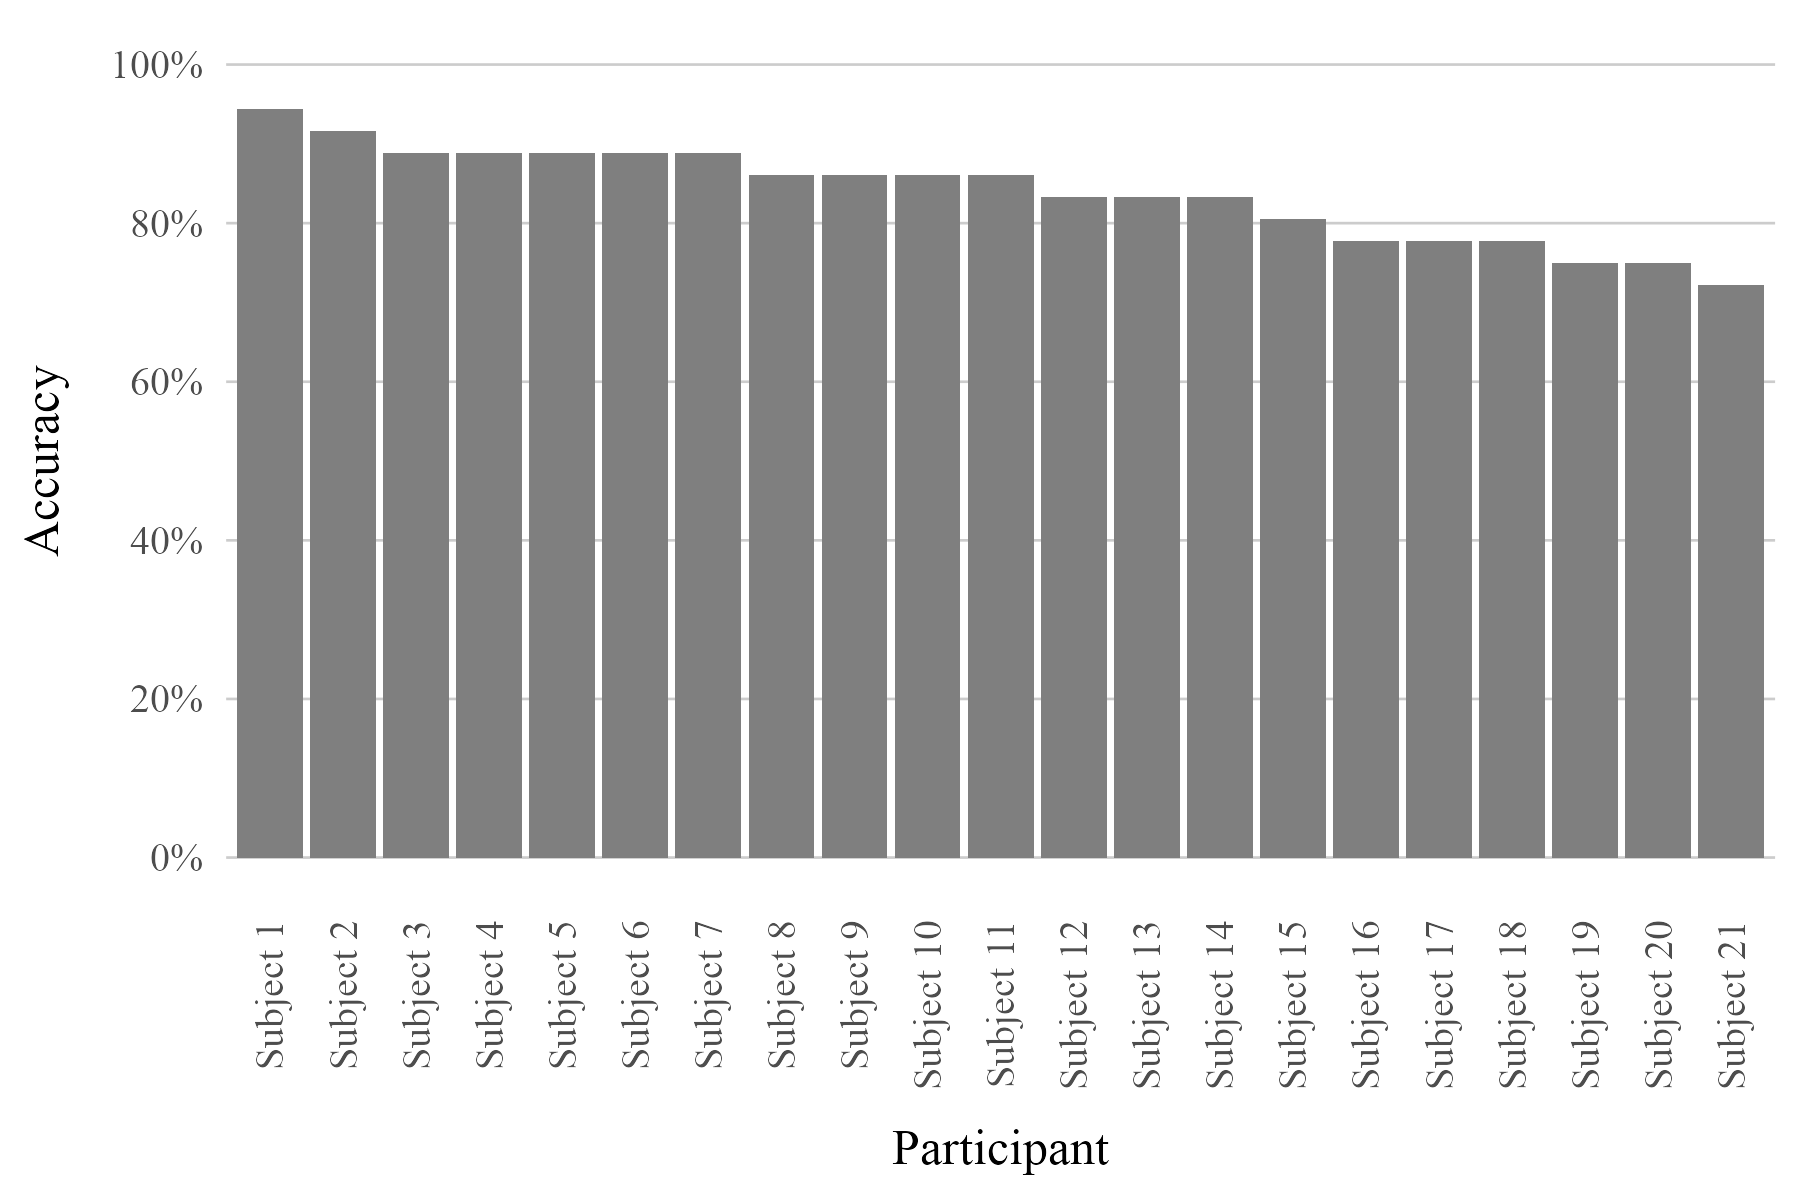
\includegraphics[width=0.8\linewidth]{comprehension_accuracy_by_participant} 

}

\caption{Mean comprehension accuracy by participant.}\label{fig:load_image}
\end{figure}

The second possible reason for the wide range of the Standard Deviation
(SD) in reading accuracy across the conditions is Item. In other words,
different target sentences might have considerable gaps in comprehension
difficulty. This could have actually happened although the target
sentences were scrutinized and balanced in number of words, structures,
and balance of meanings as whole sentences. In consequence, the top five
hardest items were screened by conditions and the results uncovered the
items with remarkably lower correct answer rates. Item No.~23 scores
persistently the lowest correct rates among the conditions (SRC-Match,
SRC-Mismatch, ORC-Match, and ORC-Mistmatch), even recorded 0\% of the
correct rate under the Condition 4. Item No.~17 and No.~19 were also
repeatedly ranked in the top 5 hardest item list. Item No.~17 was ranked
only under SRC conditions and Item No.~19 was ranked under all the
conditions except Condition 1 (SRC-Match). Especially, Item No.~23 and
No.~17 presented extremely lower correct answer rates.

Observing the sentences of Item No.~23 (example sentences 18a-d), some
potential reasons why the Item No.~23 was remarkably difficult can be
assumed. First, semantic influence might have modulated the difficulty.
In particular, the two nouns: athletes and coach(es) embrace
hierarchical image that the coach has more authority and is normally
respected and the athletes play or do some sports under the instruction
or control of the coach(es). Therefore the case when the athletes admire
the coach(es) is plausible but the opposite direction is less plausible.
Based on this hierarchy, the sentential verb, ``admire'' led the
plausible scenario of this sentence to the parsers. When the expectation
toward the meaning of the target sentence, the participants should have
got confused. Another possible reason is the relatively long modifying
phrase in the sentence, ``through many seasons''. This could have the
sentence more complex.

\vspace{1em}

\begin{longtable}[]{@{}ccccc@{}}
\caption{Top 5 Most Difficult Items by Condition}\tabularnewline
\toprule\noalign{}
Item & SRC\_Match & SRC\_Mismatch & ORC\_Match & ORC\_Mismatch \\
\midrule\noalign{}
\endfirsthead
\toprule\noalign{}
Item & SRC\_Match & SRC\_Mismatch & ORC\_Match & ORC\_Mismatch \\
\midrule\noalign{}
\endhead
\bottomrule\noalign{}
\endlastfoot
23 & 0.167 (6) & 0.250 (4) & 0.333 (6) & 0.000 (5) \\
17 & 0.333 (6) & 0.400 (5) & -- & -- \\
19 & -- & 0.500 (4) & 0.667 (6) & 0.600 (5) \\
9 & 0.667 (6) & -- & -- & -- \\
11 & 0.667 (6) & -- & -- & -- \\
29 & 0.667 (6) & -- & -- & -- \\
31 & -- & 0.500 (4) & -- & -- \\
2 & -- & 0.667 (6) & -- & 0.667 (6) \\
6 & -- & -- & 0.500 (4) & 0.667 (6) \\
28 & -- & -- & 0.600 (5) & -- \\
27 & -- & -- & 0.667 (6) & -- \\
13 & -- & -- & -- & 0.500 (4) \\
\end{longtable}

\vspace{-0.5em}
\begin{quote}
\textit{Note.} The table shows the mean correct answer rate and number of subjetcs (e.g., 0.167 (6) = mean correct answer rate was 16.7 percent and 6 participants answered this question).
\end{quote}
\vspace{1em}

\clearpage

\vspace{1em}
\noindent
\begin{tabularx}{\linewidth}{@{}l@{\hspace{0.5em}}X@{}}
(21a) & The athletes \textbf{that} admired \textbf{the coaches} through many seasons defeated opponents in the championship. \hfill \mbox{[Item No. 23 / Condition 1]} \\
(21b) & The athletes \textbf{that} admired \textbf{the coach} through many seasons defeated opponents in the championship. \hfill \mbox{[Item No. 23 / Condition 2]} \\
(21c) & The athletes \textbf{that} \textbf{the coaches} admired through many years defeated opponents in the championship. \hfill \mbox{[Item No. 23 / Condition 3]} \\
(21d) & The athletes \textbf{that} \textbf{the coach} admired through many years defeated opponents in the championship. \hfill \mbox{[Item No. 23 / Condition 4]} \\
\end{tabularx}
\vspace{1em}

\subsubsection{Summary}\label{summary-5}

In this section, the results from the GLMM and descriptive statistics
uncovered the comprehension accuracy of the Japanese EFL learners in
this study. The main finding is that the participants answered the
comprehension questions highly correctly, therefore there were no
significant main effects and interactions among Condition, English
Proficiency, and the Number of the Main Clause Subject. On the other
hand, the results of the GLMM showed wide ranges of SD by Condition.
Thus, the data was further investigated by participants. Actually, the
highest correct rate was over 90\% (correct) and the lowest was slightly
higher than 70\%. The gap between these highest and lowest scores was
relatively big, but all the participants were regarded as they
comprehended the target sentences ``good-enough'', at least they all
read the sentences and understood most of the sentences and questions.
This result also evidenced the target sentences functioned and the
participants did not skip reading and just click random keys. Besides
the individual difference in correct answer rate, individual Item was
also focused in the later analysis because the GLMM showed the random
effect, Item presented the considerable variance among them. Therefore,
the items which marked exceptionally high or low correct answer rates
were ranked. After all, the item No.~23 and 17 were found as the
extremely difficult items. All in all, the data showed no main effects
and interaction of Conditions, English Proficiency, and the Number of
the Main Clause Subject toward comprehension accuracy.

\subsection{Analysis: Reading Time}\label{analysis-reading-time}

The data were analyzed using linear mixed-effects models (LMMs) in the
lme4 package (version 1.1.37; Bates et al., 2015) in R (version 4.4.2,
2024-10-31) in order to see the relation between reading time and
conditions: RC Type, Number.Fixed effects included the experimental
factors RC Type (SRC vs.~ORC), Number (Match vs.~Mismatch), and their
interaction. Subject and Item were included as random effects in the LMM
model. The same model was applied to different regions: Region 2
(Relative Clause), Region 3 (Main Clause Verb) and Region 4 (Spillover).
The results showed the significant main effect of RC type (SRC was read
faster than ORC) at the region 2 and the main effect of Number
(sentences with number mismatch was read more quickly than the sentences
with number match) at the region 4 (Spillover). Region 3 (Main Clause
Verb) did not show any significant main effects and interaction. In the
following part of this section, the results are introduced by regions.

Region 2 (Relative Clause) contained the whole relative clause so this
region was the longest region of all which was corresponding to the
parts bracketed in the following example sentences. The order of
constituents in RC differs between SRC and ORC sentences (22a-b). SRCs
had the order as: relative pronoun (``that''), verb (``hired''), object
in RC (``the editor''), and prepositional phrase (``for the project'') .
On the other hand, ORCs had the order as: relative pronoun (``that''),
subject in RC (``the editor''), verb in RC (``hired''), and
prepositional phrase (``for the project''). Based on these different
orders of constituents, parsers would recognize the RC type and
speculate how the sentence would unfold.

\vspace{1em}
\noindent
\begin{tabular}[t]{@{}ll}
(22a) & The writer [that hired the editor for the project] revised content with great care. \hfill [SRC] \\
(22b) & The writer [that the editor hired for the project] revised content with great care. \hfill [ORC] \\
\end{tabular}

\vspace{1em}

\noindent
\begin{quote}
\small
\textit{Note.} SRC = Subject-relative clause; ORC = Object-relative clause
\end{quote}
\vspace{1em}

For the linear mixed-effects model, RC Type (SRC vs.~ORC) and Number
between the head and local NPs (Match vs.~Mismatch) and the interaction
between these were selected as fixed effects toward reading time (ms.).
In addition, the Subject (individual participant) and Item were defined
as the random effects in the model. The main effect of RC Type was
significant (\(\beta\) = 0.110, SE = 0.028, \(t\) = 3.974, \(p\) =
\textless.001). However, Number showed no significant main effect
(\(\beta\) = -0.044, SE = 0.028, \(t\) = -1.574, \(p\) = 0.116). The
interaction between RC Type and Number was also not confirmed (\(\beta\)
= -0.044, SE = -0.055, \(t\) = -0.081, \(p\) = 0.423). This result
showed that the parsers read the subject relative clauses in the
sentences more quickly than object relative clauses. Number Mismatch did
not show any facilitation effects here at region 2 (RC).

At the region 3 (Main Clause Verb), no significant main effects of RC
Type (\(\beta\) = 0.006, SE = 0.035, \(t\) = 0.165, \(p\) = 0.869) and
Number (\(\beta\) = 0.038, SE = 0.036, \(t\) = 1.058, \(p\) = 0.290) and
the interaction were confirmed (\(\beta\) = -0.013, SE = 0.070, \(t\) =
-0.178, \(p\) = 0.859). This region contained only a sole word, a verb
in the main clause. The parsers were initially expected to clarify the
attachment between the main clause subject and verb here at the region 3
because the main clause verb finally appeared at this region. Therefore,
it was hypothesized that the parsers would have shown different
performances in reading time depending on the explanatory variables and
conditions. Nevertheless, the results did not show any significant main
effects of RC Type and Number.

At the region 4 (Spillover), the significant main effect of Number
Mismatch was confirmed (\(\beta\) = -0.060, SE = 0.030, \(t\) = -2.003,
\(p\) = 0.046). This showed that the sentences with Number Mismatch
between the head and local NPs were read more quickly than the ones with
Number Match condition. However, RC Type did not show main effect
(\(\beta\) = 0.021, SE = 0.030, \(t\) = 0.700, \(p\) = 0.484). Also, the
interaction between RC Type and Number was not confirmed (\(\beta\) =
0.064, SE = 0.059, \(t\) = 1.085, \(p\) = 0.278).

To consolidate the results of region 2 (Relative Clause), 3 (Main Clause
Verb) and 4 (Spillover), the significant main effect of RC Type was
confirmed at region 2 (Relative Clause) and the significant main effect
of Number was confirmed at region 4 (Spillover). As a simple finding,
the effects of different conditions appear in different parts in the
sentences. Since region 2 (Relative Clause) contained different orders
of constituents between SRC and ORC, the main effect of RC Type (SRC
vs.~ORC) can be considered as appropriate. About the main effect of
Number (match vs.~mismatch), the main clause verb, which is equal to
region 3, should be the point where the parsers needed to clarify and
comprehend the attachment between the main clause subject and main
clause verb. Therefore, the effect of number dissimilarity (number
mismatch condition) could have been seen at region 3, however, it
appeared at region 4 (Spillover). This result could be the spillover
effect that the influence of the condition (here Number) appeared a
following part of the sentence after the targeted region. Also, it is
understandable because the region 3 (Main Clause Verb) was constituted
of a sole word, the main clause verb and the region was too short to
detect the influence of subtle difference in number.

\vspace{1em}

\begin{table}[!h]
\centering
\caption{\label{tab:Table7_LMM}Results of Linear Mixed Model (Region 2: Relative Clause)}
\centering
\begin{tabular}[t]{lrrrrr}
\toprule
Predictor / Fixed effect & Estimate & Standard error & df & t value & p value\\
\midrule
Intercept (SRC, match) & 8.338 & 0.100 & 20.350 & 83.500 & \textless{} .001\\
Number (mismatch – match) & -0.044 & 0.028 & 714.157 & -1.574 & 0.116\\
RC Type (ORC – SRC) & 0.110 & 0.028 & 699.156 & 3.974 & \textless{} .001\\
Interaction: RC × Number & -0.044 & 0.055 & 699.156 & -0.801 & 0.423\\
\bottomrule
\end{tabular}
\end{table}

\newpage

\clearpage
\thispagestyle{empty}  % ← 章扉ページはヘッダー・フッターなし
\vspace*{-1cm}
\begin{flushleft}
\Huge \textbf{Chapter 6}
\end{flushleft}
\vspace{0.3cm}
\noindent\rule{\linewidth}{0.6pt}
\pagestyle{fancy}  % ← 通常ページに戻る

\section{Discussion}\label{discussion}

\subsection{Interpretation of Results}\label{interpretation-of-results}

The results of comprehension accuracy showed no differences among
different conditions: RC Type (SRC vs.~ORC) and Number (Match
vs.~Mismatch). Simply, the most participants performed good in
comprehension (Mean correct answer rates: 83.6\% (SRC-Match); 82.0\%
(SRC-Mismatch); 85.7\% (ORC-Match); and 84.1\% (ORC-Mismatch).
Therefore, the significant differences were not confirmed. This result
was positive in a way, in particular the participants could comprehend
the sentences with relative clauses. This means the stimulus sentences
functioned well. If the comprehension accuracy was too low, the
probability would be high that the participants did not understand the
meaning of the stimuli and eventually the experiment could not collect
the targeted data properly. Thus, this result regarding the
comprehension accuracy clarified that the target sentences worked as
they were expected. On the other hand, this result was not fully along
with the initial hypothesis because the initial expected SRC condition
would lead better comprehension accuracy than ORC condition. Also, the
facilitation effect of number dissimilarity was not confirmed. This
implies that the small overt marking such as ``-s'' for plural nouns in
English is fine that the influence can not be seen clearly in tasks like
comprehension questions with yes/no choices.

In regards to the reading time analysis, the hypotheses expected there
would be the subject-object asymmetry (SRC sentences would be read more
quickly) but there would not be the facilitation effect of number
mismatch condition based on the results by Xia et al.~(2020) with
Chinese EFL learners. The results from the online self-paced reading
task, the present study supported the subject-object asymmetry and also
supported the facilitation effect of number dissimilarity toward
processing of sentences with relative clauses. To the best knowledge of
the author, the studies focusing on the facilitation effect of number
mismatch in Japanese EFL learners have not been conducted. Thus, the
supportive result from this study has novelty and at the same time is
inconsistent from the results by Xia et al.~(2020) and the hypothesis
based on their study. The current result is rather in line with other
existing studies in European languages (e.g., Adani et al., 2014;
Contemori \& Marinis, 2014).

Another noteworthy point is the main effect of RC Type (SRC vs.~ORC) and
the main effect of Number (Match vs.~Mismatch) were recorded at
significant levels at different regions in the target sentences. The
main effect of RC Type was found at Region 2 (Relative Clause). The
participants read the subject relative clauses (SRCs) faster than object
relative clauses (ORCs). This result backs up the subject-object
asymmetry which has been reported by many existing studies. There would
be some possible reasons behind this asymmetry.

In terms of the region 2 (Relative Clause), this region contains
different types of relative clauses (SRC or ORC) and was the initial
parsing stage. The participants could have expected SRC was coming than
ORC as reported some studies based on their experience and frequency
(MacDonald, 2013). In other words, SRCs appear more frequently than
ORCs, therefore, the initial expectation by parsers was accordingly SRCs
are coming at the region 2. For this reason, the parsers had some
confusion when they encountered ORCs. As stated in the earlier section,
SRCs and ORCs differed from different orders of constituents and this
caused the structural complexity. The participants could clarify whether
the sentences were SRCs or ORCs based on the different word orders. When
the input turned out to be ORCs, their initial expectation was violated
and they had confusion at the beginning of region 2. The participants
were then required syntactic reanalysis. Consequently, their parsing was
temporarily stagnated and the reading time at the region 2 became longer
than the case of SRCs. Another possible reason is the short-term memory
load, which has also been reported by different studies (J. H. Kim \&
Christianson, 2017). Meaning the parsers needed to hold the information
of the head NP longer while they were parsing ORC sentences. In the
sentences with ORCs, the head NP was the object in the relative clause.
In ORCs, the surface word order starting from the head of RC was
object-subject-verb (OSV) order unlike the usual surface word order in
English (SVO). This non-canonical word order in relative clauses could
also have generated the confusion in parsing and this required the
parsers to hold the information at longer time in their short term
memory.

Primarily, this study expected that the influences of RC Type (SRC
vs.~ORC) and Number (Match vs.~Mismatch) would have appeared at the
region 3 (Main Clause Verb) or region 4 (Spillover) because the
attachment between the main clause subject and the main clause verb
became clear at the region 3 (Main Clause Verb) once the parsers reach
the main clause verb. Before the region 3, parsers could guess the RC
type and construct the structure and meaning of the sentences, however,
the whole structure was still not perfectly revealed. Therefore, the
region 3 should have been the critical point where the parsers could
confirm the whole structure and attachment for the first time. Region 4
was set as the spillover region in case the influence of the different
conditions appeared with a bit of time lags and later than the region 3
(Main Clause Verb). The result of the present study showed there was a
significant main effect of Number at the region 4 (Spillover).So, this
can be considered as the spillover effect. The participants read the
sentence with number mismatch condition more swiftly than the ones with
number match condition. This result supported the facilitation effect of
number dissimilarity to processing the sentences with relative clauses.
As introduced in the previous section about the background of this
study, some studies supported the facilitation effect of number
dissimilarity toward RC sentences, especially ORC sentences (e.g., Adani
et al., 2014; Contemori \& Marinis, 2014; Bentea \& Burrleman, 2017).
Since those existing studies reported the facilitation effect of number
dissimilarity in european languages as L1 and L2, the result of the
current study was not only in line with those results but also added a
new case with L1 Japanese EFL learners. One of the target studies for
this study was Xia et al.~(2020). This study reported that L1 Chinese
EFL learners indicated that they read the sentences with relative
clauses faster under the number match condition between the head and
local NPs. It was opposite from the results from the other studies such
as Adani et al.~(2014) and Contemori and Marinis (2014). Although the
initial hypothesis in the present study was based on the study by Xia et
al.~(2020), the result was rather close to the other studies including
Adani et al.~(2014) and Contemori and Marinis (2014). Japanese EFL
learners utilized the number morphology as a hint in order to proceed
the relative clauses and accelerated processing. Both Chinese and
Japanese have no overt marking in number. While the L1 Chinese
participants in the study by Xia et al.~(2020) did not show any
facilitation effects, Japanese EFL learners in this study showed better
performance in number mismatch condition. The hypothesis conjectured
that the EFL learners might show influences from their first language.
However, the gap between the present study and Xia et al.~(2020)
underpinned the EFL learners whose first languages contain no number
markings could utilized the overt number between the head and local NPs
so as to process the relative clauses efficiently.

Here the question is about the possible reasons why the Chinese EFL
learners in the study by Xia et al.~(2020) did not take advantages of
number morphology and the Japanese EFL learners in the current study
did. One difference is that Chinese follows more fixed word order
without particles and Japanese is more flexible in word order with using
particles. In Japanese, parsers can rely on postnominal case markers to
identify grammatical roles such as the subject and object in the
sentences, even though the word order is relatively flexible and same
between SRCs and ORCs. In contrast, Chinese replies more heavily on word
order to grasp the grammatical roles, as it lacks overt case marking and
particles. Given that those difference in their first languages
influenced to their English processing, it is possible that Japanese EFL
learners were more sensitive toward subtle morphosyntactic cues in
sentences and might use the number mismatch between head and local NPs
and the main clause verb in order to interpret the structure and meaning
of the sentences with relative clauses.

Another possible reason behind the contrasting results of the
facilitation effect of number mismatch between Chinese EFL and Japanese
EFL learners is the difference in English instructions. In Japanese,
English class as a foreign language currently starts from the third
grade of elementary school which focuses on oral communication and
listening. Formal and systematic instruction starts in junior high
school. Basically, Japanese EFL learners learn explicit grammar here at
the junior high school. The rules regarding numbers such as ``-s'' for
plural and subject-verb agreement receive particular attention because
number systems in English do not exist in Japanese. The Japanese EFL
learners learn number related rules repeatedly and this emphasis is due
to the unfamiliarity and also the testing systems such as high school
entrance examinations that frequently ask about the number rules.
Considering this English instructional background, the Japanese EFL
learners in the present study have possibly trained themselves and been
careful with number morphology in the target sentences in this study.

\subsection{Implications}\label{implications}

The findings of this thesis not only support the existing the majority
of the theories and hypotheses with providing the novel case, but also
suggest possible practical implication in English language teaching and
cross-linguistic research in the topic.

On one hand, the results from this study supported the existence of the
subject-object asymmetry and the facilitation effect of the number
mismatch and also provided a new data with Japanese EFL learners. This
result is contributive to elevate the discussion, especially about the
facilitation of the mismatched numbers between the head and local to the
RC processing. Up until now, there are some studies focused on the
facilitation effects of the number dissimilarity, however, it is not
ample to arrive at an agreement that the facilitation effect appears
generally across the languages. Based on the result from this current
experiment, it is rather strongly required to conduct and accumulate the
cases with different language settings. In a big picture, the
accumulation helps to clarify whether the facilitation effect is a
general phenomenon regardless of languages, or it appears only under
circumstances in European languages or with specific L1 influence. The
key finding of this thesis was showing the appearance of the
facilitation effect of the number dissimilarity in English with the
participant group whose L1 has no overt number marking. This striking
finding itself supported the facilitation of number morphology happens
even among EFL learners and the facilitation effect would be a general
phenomenon. As for the future study, it is needed to compare the
Japanese EFL learners and Chinese EFL learners under the same condition.
Also, the comparison between Japanese EFL learners and native speakers
of English would also be informative.

On the other hand, the current thesis project shed light on the English
education to the Japanese EFL learners. As stated in the earlier part,
Japanese English education tends to focus on grammatical drills.
Recently, the teaching methods have been changing toward the
communicative approach, which encourages students to actively use
English in the classroom settings. The teaching method has been changed
dramatically for the last 10-15 years. This shift is to cultivate the
students' active and practical English proficiency. Nevertheless, the
testing system for high school and university entry has not been
changed, thus the grammatical drills are still required. Based on the
results of this thesis project, the Japanese EFL learenrs seemed to be
sensitive enough to utilize the number marking as the clue to process
relative clauses. This could be seen, reflecting certain characteristics
of English education in Japan, and can be viewed as a achievement. In
practical teaching, it could also be informative and helpful instructing
the students to check the numbers between the head and local nouns and
the sentential verb. Also, the instructors or teachers could teach
relative clauses based on the widely accepted asymmetry.

\subsection{Limitations}\label{limitations}

Although the significant main effects of RC Type at region 2 (Relative
Clause) and the main effect of Number at region 4 (Spillover) have been
caught, there are some methodological limitations and the results from
the present study may be limited in scope and premature to generalize as
the broad results of Japanese EFL learners. First, the participants
group in this study was relatively small (n=21) and there was no control
group with native speakers of English. The general and linguistic
backgrounds of participants were diverse because the most of them were
recruited through the online platform, whereas there is still the
possibility that the results of this study were merely specific traits
of those specific 21 participants. Second, there was no control group in
present study in order to compare with the Japanese EFL learners. Owing
to the lack of a comparison target, it was not set in stone whether the
subject-object asymmetry and the facilitation effect of number
dissimilarity found in the present study were the same as how the native
speakers of English process the relative clauses. Even though the
asymmetry was repeatedly reported by the studies with native English
speakers (Staub et al., 2017; Cunnings \& Fujita, 2023), the
facilitation effect has scarcely been observed with adult native English
speakers. Therefore, it remained unclear whether the facilitation effect
of number mismatch in this study was influenced by participants' first
language (Japanese) or it reflected the general processing pattern that
would also be observed in native English speakers. Unlike the
subject-object asymmetry, the number of studies focusing on the
facilitation effect of number dissimilarity toward the subject-object
asymmetry are still scarce and it is still unwarranted to generalize.

In addition to the limitations due to participants grouping, there were
also some constraints from the experimental methodology and the design
of the stimulus sentences. As mentioned earlier, the original
experimental plan was to conduct both the online self-paced reading task
and the normal online reading task with eye-tracking. However, the plan
had been changed because of the technical problems and time constraint.
Only the online self-paced reading task was conducted after all. One of
the biggest differences between these two methodologies is whether it is
possible to record the eye movements of regressions (backward eye
movements) and counts of fixations at the certain words or regions. The
online self-paced reading task in the present study could not record the
reading time data, especially when the participants read backwards to
reconfirm the previous parts of the sentences. In the first place, the
sentence presentation in the online self-paced reading task was not so
natural as parsers normally read the sentences because a new chunk
appeared and the previous chunk disappeared when the parsers click the
space key. Although this presentation method (non-cumulative
moving-window presentation) is designed to measure reading speed in a
controlled manner and frequently used in psycholinguistic studies, a
critical limitation is that it prevents the measurements of regressions
both in terms of frequency and duration. It was reported that the harder
sentences to process, the more frequent regression saccades and
fixations the parsers make (Rayner et al., 2006). Online self-paced
reading tasks could not record those fine and detailed eye movement
measures and also sentence presentation was not in a natural way.

Alongside the overall experimental method, the stimulus sentences had
some limitation. The most of the target sentences were referred and
edited by Staub et al.~(2017) and the number condition between the head
and local nouns was added. The main limitation in the present study was
the control of the semantic roles of the words used in the target
sentences, particularly the head and local nouns. The meanings of the
whole sentences were controlled as they were categorized positive,
negative, and neutral groups and deployed equally. However, certain
sentences were obviously too difficult for the participants such as Item
No.23 and No.17. Also, the words used in the target sentences were
controlled in terms of their semantic roles and collective nouns were
excluded. One limitation is that the semantic roles between the head and
the local nouns were not fully controlled or examined. For instance, the
example sentence below has ``the doctors'' as the head NP and ``the
patient'' as the local NP. In comparison between the semantic roles of
these two NPs, ``the doctor'' tends to have an agent role and ``the
patient'' is likely to be patient role. Only with seeing these two NPs,
parsers could recognize how the sentence will unfold and easily
determine the semantic relation between the head and local nouns and
which should be attached to the main clause verb. In the present study,
adjustments were made to ensure that the overall meaning of the whole
text was not biased, nevertheless, it must be acknowledged that the
semantic roles of the head and local NPs were insufficiently checked and
revised. Consequently, in some sentences---like the one below---the
lexical relationship between the head and local NPs might have clarified
their semantic roles, possibly serving as a hint to the parsers.

\vspace{1em}
\setlength{\parindent}{0pt}
\noindent
\begin{tabular}[t]{@{}ll}
(23) & The doctors that greeted the patient in the lobby provided guidance on treatment options. \\
\end{tabular}
\vspace{1em}

\subsection{Suggestions for the Future
Research}\label{suggestions-for-the-future-research}

\setlength{\parindent}{1.27cm}

Based on the results and limitations of the present studies, some points
to improve have been delineated. From the methodological viewpoint, the
study should combine multiple ways of experiments to verify especially
the facilitation effect of number mismatch with different experiments.
The present study detected the significant facilitation effect of the
number dissimilarity at region 4 (Spillover), however, there remains a
concern that the observed effect may have occurred by chance. If
multiple experimental methods were applied to the same or homogeneous
group of participants under identical conditions and stimuli, it would
become possible to comparatively decide whether the asymmetry and the
facilitation effect of number dissimilarity can be observed across
methods and how robust the results are. For the next step, both the
online self-paced reading tasks and online normal reading tasks with
eye-tracking can be combined, thereby the possible subject-object
asymmetry and the facilitation effect of the number mismatch can be
confirmed and discussed from different perspectives. For instance, the
frequency and duration of regression saccades and fixations will be
provided by the eye-tracking task. These could not be given if only the
self-paced reading task were conducted. Although Region 3 (Main Clause
Verb) was the critical region where the facilitation effect of the
number dissimilarity could have been observed, the region contained only
one word. The effect could be recorded later with some time rag.
Therefore, the multifaceted results from different experiments are
needed. Actually, some of the studies combined different tasks (Xia et
al., 2020).

For further improvement, the experimental stimuli could also be refined
in several respects in future research. For example, the semantic roles
of the head and local NPs could be more carefully screened and
controlled; the same lexical items could be used across conditions (RC
Type and Number) and lexical items placed as the head and local nouns
that dictate the meaning and structure of the whole sentence should be
prevented from being used in the target sentences. In addition, the main
clause verb that make the relationship between the two NPs too
transparent should also be avoided to use. To illustrate, take a
sentence like one where the head NP is ``fan'', the local NP is
``musician'', and the main verb is `photographed'. The verb strongly
hints at the likely thematic roles of those two nouns, thus undermining
the intended ambiguity. Consequently, the target sentences would differ
in terms of processing complexity and difficulty. In this case, the verb
``photographed'' is likely to be attached with the noun ``fan'' rather
than the noun ``musician'' and semantic plausibility may clearly suggest
which noun is more likely to be the agent or patient, thereby reducing
the ambiguity as stimuli.

In respect of the participants, the control group needs to be added in
the study so that the subject-object asymmetry and the possible
facilitation effect can be examined comparatively. Particularly, the
studies focusing on the facilitation effect of the number dissimilarity
are still scarce and many of them have viewpoints from developmental
linguistics and clinical linguistics (Adani et al., 2014). A majority of
existing studies focusing on the facilitation effect of number
morphology recruited the children monolingual or bilingual participants
and the others recruited participants with G-SLI (grammatical specific
language impaired). Surprisingly, the studies with adult native speakers
of English without G-SLI have not been observed to the best knowledge of
the author. Considering the current situation, adding the participant
group of native speakers of English would contribute to the extension of
the study in two ways. First, the data of the native English speakers
would be the benchmark whether the number morphology including the
plural marker ``-s'' on the noun is used as a clue to process the
sentences with relative clauses. Many studies supported the noun types
(e.g., descriptives and pronouns), semantic relatedness between the head
and local nouns, frequency of used words would also play the role of
determining the processing difficulty of the relative clause sentences
with native speakers of English (e.g., Gordon et al, 2004; Lowder et
al., 2014; Johnson et al., 2011). It has been revealed that native
speakers of English utilize the subtle markers or difference between the
head and local nouns to comprehend the sentences with relative clause
faster and more accurately. It is meaningful to accumulate the studies
about the facilitation effect of the number dissimilarity with different
methodologies and participant groups of native English speakers.

Another contribution from adding the participant group of native English
speaker to this study is to build on the comparability with the target
group (Japanese EFL learners). The result of the current study provided
only the results of Japanese EFL learners. The results provided some new
findings such that Japanese EFL learners whose first language does not
have number morphology and overt marking also utilized the number
mismatch to proceed the relative clause. This result itself was actually
informative however it remains unclear whether this facilitation effect
also occurs in adult native speakers of English or if it is particular
to Japanese EFL learners who participated in the present study. Without
comparative data or accumulated pre-existing studies in this topic,
underlying mechanism cannot be pinpointed. Therefore, recruitment of the
group of English native speakers is essential for the further study and
improvement. If similar results were observed in the native speaker
group, the facilitation effect of the number dissimilarity would reflect
a more general pattern and the EFL learners were supposed to learn to
utilize the number marking as a cue to interpret sentences with relative
clauses. In this case, the influence of the EFL learners' first language
would appear to be minimal. On the other hand, if native speakers and
Japanese EFL learners exhibit divergent processing patterns related to
the facilitation effect of the number dissimilarity, it would be
reasonable to consider that L1-specific factors such as structural
characteristics of Japanese or the effects of grammar-focused English
instruction of English education at school in Japan may shape the
processing strategy of the Japanese EFL learners.

Apart from the areas of improvements based on the present study,
studying the relationship between the subject-object asymmetry and
number morphology is still a blue ocean. In brief, it is indispensable
to conduct and accumulate the empirical data with different participant
groups and methodologies. With the exception of certain studies focusing
on Chinese, a wide range of previous research has reached a shared
understanding regarding the existence of the subject-object asymmetry.
As a result, numerous studies can serve as valid points of comparison
when conducting replication studies of subject-object asymmetry with
different participant groups. Although there is also a substantial body
of studies about the number agreement including subject-verb agreement,
far fewer studies have examined how subtle lexical markers such as
number or gender effect the processing of relative clauses. As the
studies about the facilitation effect of subtle morphological markers
such number or gender are piled up, the shared and plausible
interpretation of the facilitation effects of number dissimilarity would
be constructed.

\newpage

\clearpage
\thispagestyle{empty}  % ← 章扉ページはヘッダー・フッターなし
\vspace*{-1cm}
\begin{flushleft}
\Huge \textbf{Chapter 7}
\end{flushleft}
\vspace{0.3cm}
\noindent\rule{\linewidth}{0.6pt}
\pagestyle{fancy}  % ← 通常ページに戻る

\section{Conclusion}\label{conclusion}

The present study had two research questions. The first question was
whether the Japanese EFL learners show the subject-object asymmetry
during reading sentences with relative clauses in English and the second
question was whether the number mismatch condition between the head and
local NPs props relative clause processing. The first point with the
subject-object asymmetry has been studied by many scholars with
different participant populations and methodologies, however, the
facilitation effect of the number dissimilarity, which is the second
point in this study, has not been studied and is still lacking enough
reference cases with different target languages, participants and
methodology. The present study conducted the online self-paced reading
task and the questionnaire regarding the participants' general and
language-related backgrounds. Based on the reading time and
comprehension accuracy data from the online self-paced reading task, the
Japanese EFL learners showed the subject-object asymmetry, especially in
reading time at the region 2 (Relative Clause). No significant
differences among the conditions were confirmed in comprehension
accuracy because the participants' comprehension was relatively accurate
regardless of the conditions. In respect to the second question about
the facilitation effect of the number dissimilarity, the hypothesis was
weaved based on the results of Xia et al.~(2020) because the condition
was relatively similar as the participants were L1 Chinese EFL learners
and the target language was English. Although the hypothesis predicted
there would not be the facilitation effect of the number dissimilarity
toward relative clause processing, the experimental results of the
present study indicated there was a facilitation effect of number
dissimilarity in reading time at the region 4 (Spillover). Both Japanese
and Chinese as the first language of the participants in this study and
Xia et al.~(2020) have no overt markers of number. Thus, the initial
hypothesis toward the second research question was rejected.

Considering the results of those two themes of the current study:
subject-object asymmetry and facilitation effect of number
dissimilarity, the present study showed the result about the
subject-object asymmetry which is conforming to the previous studies
with Japanese EFL learners (e.g., Narumi \& Yokokawa, 2013; Hashimoto \&
Hirai, 2007). In terms of the facilitation effect of the number
mismatch, the present study provided a new case and data with Japanese
EFL learners and supported the facilitation effect of the number
dissimilarity. In addition, the result supporting the facilitation
effect of the number mismatch attracted the discussion whether the
facilitation effect of the number morphology draws influence from the
first languages such as existence or absence of overt number markers, or
the facilitation effect is rather a general phenomenon in Indo-European
languages including English. The bottle neck of this discussion is the
lack of direct referable studies, especially EFL/L2 studies with
participants whose first languages are not Indo-European languages and
containing no overt number marking system. To the best knowledge of the
author, there has been no study focusing on the facilitation effect of
number morphology in relative clause processing with Japanese EFL
learners. Referring to the existing resemble studies, Cilibrasi et
al.~(2022) confirmed the facilitation effect of the number dissimilarity
with English-Czech bilingual children, however, Xia et al.~(2020) did
not confirmed the facilitation effects of the number mismatch of the
number mismatch in L1 Chinese EFL learners and even upheld the L1
Chinese EFL learners performed better under the number match condition.
Cilibrasi et al.~(2022) opined the contrasting result reported by Xia et
al.~(2020) was because the L1 Chinese EFL was not so sensitive enough to
utilize the number marker as a hint during the processing of relative
clauses due to the trait of Chinese. The insight by Cilibrasi et
al.~(2022) and the results from Xia et al.~(2020) signaled the
possibility the traits in the first languages would influence the
facilitation effect of the number dissimilarity. On the other hand, the
result of the current study backed up the facilitation effect of the
number mismatch in Japanese EFL learners.

As a provisional conclusion, the facilitation effect appears to be a
more frequently observed phenomenon among both native speakers and
foreign language learners in Indo-European languages. However, in the
case of EFL or L2/EFL learners, it is possible that the characteristics
of their first language and the learning process have a significant
influence. For the further research, conducting the the same task
(online self-paced reading task) and other tasks such as eye-tracking
with native English speakers is necessary. Furthermore, verifying the
subject-object asymmetry and especially the facilitation effect of
morphological markers including number in different language settings is
needed.

In conclusion, this master's thesis project successfully yielded the
novel findings that contribute to future research, especially about the
facilitation effect of number mismatch toward relative clause
processing. First, this study supported the existence of the
subject-object asymmetry as reported in the majority of the existing
studies across languages. Besides that, this thesis confirmed the
facilitation effect of number mismatch to the relative clause processing
by the Japanese EFL learners. This second finding provided a novel case.
On the other hand, expanding the participant groups and revising the
experimental stimuli are necessary for the further improvement of the
study. As a next goal, it is aimed to conduct a comparison between
native English speakers and Japanese EFL learners of English, so that it
will be verified whether the patterns observed in this thesis project
with Japanese EFL leaners also appear among native speakers.

\clearpage
\markboth{References}{References}

\section*{References}\label{references}
\addcontentsline{toc}{section}{References}

\phantomsection\label{refs}
\begin{CSLReferences}{1}{0}
\bibitem[\citeproctext]{ref-AbdolmanafiRahmani2012}
Abdolmanafi, S. J., \& Rahmani, Z. (2012). An investigation of the
learnability of relative clauses by EFL learners. \emph{World Journal of
English Language}, \emph{2}(3), 29.

\bibitem[\citeproctext]{ref-AdaniEtAl2014}
Adani, F., Forgiarini, M., Guasti, M. T., \& Van Der Lely, H. K. (2014).
Number dissimilarities facilitate the comprehension of relative clauses
in children with (grammatical) specific language impairment.
\emph{Journal of Child Language}, \emph{41}(4), 811--841.

\bibitem[\citeproctext]{ref-Al-MaaniAl-Haija2019}
Al-Maani, A., \& Al-Haija, L. A. (2019). The acquisition of english
relative clauses by university students of english in jordan.
\emph{Jordanian Educational Journal}, \emph{4}(1), 1--19.

\bibitem[\citeproctext]{ref-Alotaibi2016}
Alotaibi, A. M. (2016). Examining the learnability of english relative
clauses: Evidence from kuwaiti EFL learners. \emph{English Language
Teaching}, \emph{9}(2), 57--65.

\bibitem[\citeproctext]{ref-Arnon2010}
Arnon, I. (2010). Rethinking child difficulty: The effect of NP type on
children's processing of relative clauses in hebrew. \emph{Journal of
Child Language}, \emph{37}(1), 27--57.

\bibitem[\citeproctext]{ref-BatesEtAl2015}
Bates, D., Mächler, M., Bolker, B., \& Walker, S. (2015). Fitting linear
mixed-effects models using lme4. \emph{Journal of Statistical Software},
\emph{67}, 1--48.

\bibitem[\citeproctext]{ref-BenteaBurrleman2017}
Bentea, A., \& Durrleman, S. (2017). Now you hear it, now you don't:
Number mismatch in the comprehension of relative clauses in french.
\emph{Proceedings of the 41st Annual Boston University Conference on
Language Development}, 60--73.

\bibitem[\citeproctext]{ref-Bever1970}
Bever, T. (1970). \emph{The cognitive basis for linguistic structures}
(pp. 279--352).
\url{https://doi.org/10.1093/acprof:oso/9780199677139.003.0001}

\bibitem[\citeproctext]{ref-BiondoEtAl2023}
Biondo, N., Pagliarini, E., Moscati, V., Rizzi, L., \& Belletti, A.
(2023). Features matter: The role of number and gender features during
the online processing of subject-and object-relative clauses in italian.
\emph{Language, Cognition and Neuroscience}, \emph{38}(6), 802--820.

\bibitem[\citeproctext]{ref-BockMiller1991}
Bock, K., \& Miller, C. A. (1991). Broken agreement. \emph{Cognitive
Psychology}, \emph{23}(1), 45--93.

\bibitem[\citeproctext]{ref-CarreirasEtAl2010}
Carreiras, M., Duñabeitia, J. A., Vergara, M., De La Cruz-Pavı́a, I., \&
Laka, I. (2010). Subject relative clauses are not universally easier to
process: Evidence from basque. \emph{Cognition}, \emph{115}(1), 79--92.

\bibitem[\citeproctext]{ref-Chang2004}
Chang, Y.-F. (2004). Second language relative clause acquisition: An
examination of cross-linguistic influences. \emph{Online Submission}.

\bibitem[\citeproctext]{ref-CilibrasiEtAl2022}
Cilibrasi, L., Adani, F., Pérez, A. I., Schmidt, E., Wigdorowitz, M., \&
Tsimpli, I. M. (2022). The role of number mismatch and exposure in the
comprehension of relative clauses in bilingual children. \emph{Applied
Psycholinguistics}, \emph{43}(3), 663--682.

\bibitem[\citeproctext]{ref-ClahsenFelser2006}
Clahsen, H., \& Felser, C. (2006). Continuity and shallow structures in
language processing. \emph{Applied Psycholinguistics}, \emph{27}(1),
107--126.

\bibitem[\citeproctext]{ref-CohenMehler1996}
Cohen, L., \& Mehler, J. (1996). Click monitoring revisited: An on-line
study of sentence comprehension. \emph{Memory \& Cognition}, \emph{24},
94--102.

\bibitem[\citeproctext]{ref-ComrieKeenan1979}
Comrie, B., \& Keenan, E. L. (1979). Noun phrase accessibility
revisited. \emph{Language}, 649--664.

\bibitem[\citeproctext]{ref-ContemoriMarinis2014}
Contemori, C., \& Marinis, T. (2014). The impact of number mismatch and
passives on the real-time processing of relative clauses. \emph{Journal
of Child Language}, \emph{41}(3), 658--689.

\bibitem[\citeproctext]{ref-CunningsFujita2023}
Cunnings, I., \& Fujita, H. (2023). Similarity-based interference and
relative clauses in second language processing. \emph{Second Language
Research}, \emph{39}(2), 539--563.

\bibitem[\citeproctext]{ref-Edeleva2023}
Edeleva, J. (2023). Embedded NP error in german object relative clause
comprehension: A case for a universal developmental pathway.
\emph{Quarterly Journal of Experimental Psychology}, \emph{76}(6),
1220--1232.

\bibitem[\citeproctext]{ref-EF2024}
EF Education First. (2024). \emph{EF english proficiency index 2024}.
\url{https://www.ef.com/wwen/epi/}.

\bibitem[\citeproctext]{ref-Ferreira2003}
Ferreira, F. (2003). The misinterpretation of noncanonical sentences.
\emph{Cognitive Psychology}, \emph{47}(2), 164--203.

\bibitem[\citeproctext]{ref-FriedmannEtAl2009}
Friedmann, N., Belletti, A., \& Rizzi, L. (2009). Relativized relatives:
Types of intervention in the acquisition of a-bar dependencies.
\emph{Lingua}, \emph{119}(1), 67--88.

\bibitem[\citeproctext]{ref-Gao2014}
Gao, Q.-Q. (2014). Chinese EFL learners' acquisition of english relative
clauses. \emph{International Journal of English Linguistics},
\emph{4}(3), 82.

\bibitem[\citeproctext]{ref-GennariMacDonald2008}
Gennari, S. P., \& MacDonald, M. C. (2008). Semantic indeterminacy in
object relative clauses. \emph{Journal of Memory and Language},
\emph{58}(2), 161--187.

\bibitem[\citeproctext]{ref-GennariMacDonald2009}
Gennari, S. P., \& MacDonald, M. C. (2009). Linking production and
comprehension processes: The case of relative clauses. \emph{Cognition},
\emph{111}(1), 1--23.

\bibitem[\citeproctext]{ref-Gibson2000}
Gibson, E. (2000). The dependency locality theory: A distance-based
theory of linguistic complexity. \emph{Image, Language, Brain},
\emph{2000}, 95--126.

\bibitem[\citeproctext]{ref-GibsonWu2013}
Gibson, E., \& Wu, H.-H. I. (2013). Processing chinese relative clauses
in context. \emph{Language and Cognitive Processes}, \emph{28}(1-2),
125--155.

\bibitem[\citeproctext]{ref-GordonEtAl2001}
Gordon, P. C., Hendrick, R., \& Johnson, M. (2001). Memory interference
during language processing. \emph{Journal of Experimental Psychology:
Learning, Memory, and Cognition}, \emph{27}(6), 1411.

\bibitem[\citeproctext]{ref-GordonEtAl2004}
Gordon, P. C., Hendrick, R., \& Johnson, M. (2004). Effects of noun
phrase type on sentence complexity. \emph{Journal of Memory and
Language}, \emph{51}(1), 97--114.

\bibitem[\citeproctext]{ref-GrodnerGibson2005}
Grodner, D., \& Gibson, E. (2005). Consequences of the serial nature of
linguistic input for sentenial complexity. \emph{Cognitive Science},
\emph{29}(2), 261--290.

\bibitem[\citeproctext]{ref-Hamilton1994}
Hamilton, R. L. (1994). Is implicational generalization unidirectional
and maximal? Evidence from relativization... \emph{Language Learning},
\emph{44}(1).

\bibitem[\citeproctext]{ref-HashimotoHirai2007}
Hashimoto, K., \& Hirai, A. (2007). Comprehension of post-modification
structures by japanese learners of english: An analysis by detailed
reading time. \emph{ARELE: Annual Review of English Language Education
in Japan}, \emph{18}, 201--210.

\bibitem[\citeproctext]{ref-Hassan2018}
Hassan, I. H. (2018). Investigating the acquisition order of english
restrictive relative clauses: Evidence from egyptian EFL learners.
\emph{Journal of the Faculty of Education at Alexandria University},
\emph{28}(1), 313--343.

\bibitem[\citeproctext]{ref-Hayashi2019}
Hayashi, S. (2019). An examination of difficulty levels in
grammaticality judgment of english relative clauses. \emph{Fukuoka
Daigaku Kenkyubu Ronshu A: Jinbun Kagaku Hen}, \emph{19}(1), 17--22.

\bibitem[\citeproctext]{ref-Hopp2016}
Hopp, H. (2016). The timing of lexical and syntactic processes in second
language sentence comprehension. \emph{Applied Psycholinguistics},
\emph{37}(5), 1253--1280.

\bibitem[\citeproctext]{ref-Ishizuka2005}
Ishizuka, T. (2005). Processing relative clauses in japanese. \emph{UCLA
Working Papers in Linguistics}, \emph{13}, 135--157.

\bibitem[\citeproctext]{ref-IshizukaEtAl2003}
Ishizuka, T., Nakatani, K., \& Gibson, E. (2003). Relative clause
extraction complexity in japanese. \emph{Poster Presented at the 16th
Annual CUNY Conference on Human Sentence Processing, Massachusetts
Institute of Technology, Cambridge, MA}.

\bibitem[\citeproctext]{ref-Izumi2003}
Izumi, S. (2003). Processing difficulty in comprehension and production
of relative clauses by learners of english as a second language.
\emph{Language Learning}, \emph{53}(2), 285--323.

\bibitem[\citeproctext]{ref-JamesEtAl2018}
James, A. N., Fraundorf, S. H., Lee, E.-K., \& Watson, D. G. (2018).
Individual differences in syntactic processing: Is there evidence for
reader-text interactions? \emph{Journal of Memory and Language},
\emph{102}, 155--181.

\bibitem[\citeproctext]{ref-JohnsonEtAl2011}
Johnson, M. L., Lowder, M. W., \& Gordon, P. C. (2011). The
sentence-composition effect: Processing of complex sentences depends on
the configuration of common noun phrases versus unusual noun phrases.
\emph{Journal of Experimental Psychology: General}, \emph{140}(4), 707.

\bibitem[\citeproctext]{ref-KahramanSakai2015}
Kahraman, B., \& Sakai, H. (2015). Relative clause processing in
japanese: Psycholinguistic investigation into typological differences.
\emph{Handbook of Japanese Psycholinguistics}, 423--456.

\bibitem[\citeproctext]{ref-KahramanEtAl2011}
Kahraman, B., Sato, A., Ono, H., \& Sakai, H. (2011). Incremental
processing of gap-filler dependencies: Evidence from the processing of
subject and object clefts in japanese. \emph{The Proceeding of the
Twelfth Tokyo Conference on Psycholinguistics}, \emph{113147}.

\bibitem[\citeproctext]{ref-Kanno2007}
Kanno, K. (2007). Factors affecting the processing of japanese relative
clauses by L2 learners. \emph{Studies in Second Language Acquisition},
\emph{29}(2), 197--218.

\bibitem[\citeproctext]{ref-KiddEtAl2007}
Kidd, E., Brandt, S., Lieven, E., \& Tomasello, M. (2007). Object
relatives made easy: A cross-linguistic comparison of the constraints
influencing young children's processing of relative clauses.
\emph{Language and Cognitive Processes}, \emph{22}(6), 860--897.

\bibitem[\citeproctext]{ref-KiddEtAl2015}
Kidd, E., Chan, A., \& Chiu, J. (2015). Cross-linguistic influence in
simultaneous cantonese--english bilingual children's comprehension of
relative clauses. \emph{Bilingualism: Language and Cognition},
\emph{18}(3), 438--452.

\bibitem[\citeproctext]{ref-Kim2017}
Kim, C.-E. (2017). Korean EFL learners' production of english relative
clauses. \emph{The Modern English Society}, \emph{18}, 71--85.
\url{https://doi.org/10.18095/meeso.2017.18.2.04}

\bibitem[\citeproctext]{ref-KimChristianson2017}
Kim, J. H., \& Christianson, K. (2017). Working memory effects on L1 and
L2 processing of ambiguous relative clauses by korean L2 learners of
english. \emph{Second Language Research}, \emph{33}(3), 365--388.

\bibitem[\citeproctext]{ref-KingJust1991}
King, J., \& Just, M. A. (1991). Individual differences in syntactic
processing: The role of working memory. \emph{Journal of Memory and
Language}, \emph{30}(5), 580--602.

\bibitem[\citeproctext]{ref-Kortmann2020}
Kortmann, B. (2020). English linguistics. \emph{Essentials. JB Metzler}.

\bibitem[\citeproctext]{ref-Kuno1974}
Kuno, S. (1974). The position of relative clauses and conjunctions.
\emph{Linguistic Inquiry}, \emph{5}(1), 117--136.

\bibitem[\citeproctext]{ref-KwonEtAl2010}
Kwon, N., Gordon, P. C., Lee, Y., Kluender, R., \& Polinsky, M. (2010).
Cognitive and linguistic factors affecting subject/object asymmetry: An
eye-tracking study of prenominal relative clauses in korean.
\emph{Language}, \emph{86}(3), 546--582.

\bibitem[\citeproctext]{ref-LowderGordon2014}
Lowder, M. W., \& Gordon, P. C. (2014). Effects of animacy and
noun-phrase relatedness on the processing of complex sentences.
\emph{Memory \& Cognition}, \emph{42}, 794--805.

\bibitem[\citeproctext]{ref-MacDonald2013}
MacDonald, M. C. (2013). How language production shapes language form
and comprehension. \emph{Frontiers in Psychology}, \emph{4}, 226.

\bibitem[\citeproctext]{ref-MacDonaldChristiansen2002}
MacDonald, M. C., \& Christiansen, M. H. (2002). \emph{Reassessing
working memory: Comment on just and carpenter (1992) and waters and
caplan (1996).}

\bibitem[\citeproctext]{ref-MakEtAl2002}
Mak, W. M., Vonk, W., \& Schriefers, H. (2002). The influence of animacy
on relative clause processing. \emph{Journal of Memory and Language},
\emph{47}(1), 50--68.

\bibitem[\citeproctext]{ref-MakEtAl2006}
Mak, W. M., Vonk, W., \& Schriefers, H. (2006). Animacy in processing
relative clauses: The hikers that rocks crush. \emph{Journal of Memory
and Language}, \emph{54}(4), 466--490.

\bibitem[\citeproctext]{ref-MansbridgeTamaoka2019}
Mansbridge, M. P., \& Tamaoka, K. (2019). Ambiguity in japanese relative
clause processing. \emph{Journal of Japanese Linguistics}, \emph{35}(1),
75--136.

\bibitem[\citeproctext]{ref-MarefatRahmany2009}
Marefat, H., \& Rahmany, R. (2009). Acquisition of english relative
clauses by persian EFL learners. \emph{Journal of Language and
Linguistic Studies}, \emph{5}(2).

\bibitem[\citeproctext]{ref-McElreeEtAl2003}
McElree, B., Foraker, S., \& Dyer, L. (2003). Memory structures that
subserve sentence comprehension. \emph{Journal of Memory and Language},
\emph{48}(1), 67--91.

\bibitem[\citeproctext]{ref-MiyamotoNakamura2013}
Miyamoto, E. T., \& Nakamura, M. (2013). Unmet expectations in the
comprehension of relative clauses in japanese. \emph{Proceedings of the
Annual Meeting of the Cognitive Science Society}, \emph{35}.

\bibitem[\citeproctext]{ref-Muranoi2016}
Muranoi, H. (2016). Development of a diagnostic test to measure japanese
EFL learners' grammatical competence. \emph{Tohoku Gakuin University
Ronshu: English Language \& Literature}, \emph{100}, 1--44.

\bibitem[\citeproctext]{ref-Nakamori2002}
Nakamori, T. (2002). Teaching relative clauses: How to handle a bitter
lemon for japanese learners and english teachers. \emph{ELT Journal},
\emph{56}(1), 29--40.

\bibitem[\citeproctext]{ref-NarumiYokokawa2013}
Narumi, T., \& Yokokawa, H. (2013). Proficiency and working memory
effects on the use of animacy and morphosyntactic information in
comprehending temporarily ambiguous sentences by japanese EFL learners:
An eye-tracking study. \emph{Journal of the Japan Society for Speech
Sciences}, \emph{14}, 19--42.

\bibitem[\citeproctext]{ref-NicolEtAl1997}
Nicol, J. L., Forster, K. I., \& Veres, C. (1997). Subject-verb
agreement processes in comprehension. \emph{Journal of Memory and
Language}, \emph{36}(4), 569--587.

\bibitem[\citeproctext]{ref-OGradyEtAl2003}
O'Grady, W., Lee, M., \& Choo, M. (2003). A subject-object asymmetry in
the acquisition of relative clauses in korean as a second language.
\emph{Studies in Second Language Acquisition}, \emph{25}(3), 433--448.

\bibitem[\citeproctext]{ref-OewerdieckEtAl2021}
Öwerdieck, D., Hamann, C., Ibrahim, L. A., Dionne, D., \& Vidal Covas,
L. (2021). Studying a bilingual population's production and
comprehension of relative clauses longitudinally: Preliminary results.
\emph{Proceedings of the 45th Annual Boston University Conference on
Language Development}, 40--51.

\bibitem[\citeproctext]{ref-Prolific}
Prolific. (n.d.). \emph{Prolific: Participant recruitment for research}.
\url{https://www.prolific.com}.

\bibitem[\citeproctext]{ref-RaynerEtAl2006}
Rayner, K., Chace, K. H., Slattery, T. J., \& Ashby, J. (2006). Eye
movements as reflections of comprehension processes in reading.
\emph{Scientific Studies of Reading}, \emph{10}(3), 241--255.

\bibitem[\citeproctext]{ref-Reali2014}
Reali, F. (2014). Frequency affects object relative clause processing:
Some evidence in favor of usage-based accounts. \emph{Language
Learning}, \emph{64}(3), 685--714.

\bibitem[\citeproctext]{ref-RealiChristiansen2007}
Reali, F., \& Christiansen, M. H. (2007). Processing of relative clauses
is made easier by frequency of occurrence. \emph{Journal of Memory and
Language}, \emph{57}(1), 1--23.

\bibitem[\citeproctext]{ref-Rizzi2001}
Rizzi, L. (2001). Relativized minimality effects. \emph{The Handbook of
Contemporary Syntactic Theory}, 89--110.

\bibitem[\citeproctext]{ref-RungruangChanthawee2023}
Rungruang, A., \& Chanthawee, C. (2023). The effects of explicit
instruction on english relative clauses. \emph{Trends of Humanities and
Social Sciences Research}, \emph{11}(1), 67--96.

\bibitem[\citeproctext]{ref-SakakibaraYokokawa2015}
Sakakibara, K., \& Yokokawa, H. (2015). Repeated exposure effects on
japanese EFL learners' relative clause processing: Evidence from a
self-paced reading experiment. \emph{Journal of the Japan Society for
Speech Sciences}, \emph{16}, 35--58.

\bibitem[\citeproctext]{ref-SatoEtAl2012}
Sato, A., Kahraman, B., \& Sakai, H. (2012). When is the object relative
clause easier to process than the subject relative clause?
\emph{Technical Report of IEICE: Thought and Language (TL)},
\emph{112}(145), 41--46.

\bibitem[\citeproctext]{ref-SchriefersEtAl1995}
Schriefers, H., Friederici, A. D., \& Kuhn, K. (1995). The processing of
locally ambiguous relative clauses in german. \emph{Journal of Memory
and Language}, \emph{34}(4), 499--520.

\bibitem[\citeproctext]{ref-Sheldon1974}
Sheldon, A. (1974). The role of parallel function in the acquisition of
relative clauses in english. \emph{Journal of Verbal Learning and Verbal
Behavior}, \emph{13}(3), 272--281.

\bibitem[\citeproctext]{ref-Staub2010}
Staub, A. (2010). Eye movements and processing difficulty in object
relative clauses. \emph{Cognition}, \emph{116}(1), 71--86.

\bibitem[\citeproctext]{ref-StaubEtAl2017}
Staub, A., Dillon, B., \& Clifton Jr, C. (2017). The matrix verb as a
source of comprehension difficulty in object relative sentences.
\emph{Cognitive Science}, \emph{41}, 1353--1376.

\bibitem[\citeproctext]{ref-StellaEngelhardt2021}
Stella, M., \& Engelhardt, P. E. (2021). Comprehension and eye movements
in the processing of subject-and object-relative clauses: Evidence from
dyslexia and individual differences. \emph{Brain Sciences},
\emph{11}(7), 915.

\bibitem[\citeproctext]{ref-Street2017}
Street, J. A. (2017). This is the native speaker that the non-native
speaker outperformed: Individual, education-related differences in the
processing and interpretation of object relative clauses by native and
non-native speakers of english. \emph{Language Sciences}, \emph{59},
192--203.

\bibitem[\citeproctext]{ref-SunEtAl2023}
Sun, L., Fan, L., \& Xu, M. (2023). Exploring the effects of animacy and
verb type on the processing asymmetry between SRC and ORC among chinese
EFL learners. \emph{Humanities and Social Sciences Communications},
\emph{10}(1), 1--10.

\bibitem[\citeproctext]{ref-Takahashi2018}
Takahashi, Y. (2018). A corpus-based study on japanese EFL learners' use
of relative clause constructions: CEFR criterial feature and error
analysis. \emph{English Corpus Studies}, \emph{25}, 57--78.

\bibitem[\citeproctext]{ref-TraxlerEtAl2002}
Traxler, M. J., Morris, R. K., \& Seely, R. E. (2002). Processing
subject and object relative clauses: Evidence from eye movements.
\emph{Journal of Memory and Language}, \emph{47}(1), 69--90.

\bibitem[\citeproctext]{ref-UenoGarnsey2008}
Ueno, M., \& Garnsey, S. M. (2008). An ERP study of the processing of
subject and object relative clauses in japanese. \emph{Language and
Cognitive Processes}, \emph{23}(5), 646--688.

\bibitem[\citeproctext]{ref-VanDykeMcElree2006}
Van Dyke, J. A., \& McElree, B. (2006). Retrieval interference in
sentence comprehension. \emph{Journal of Memory and Language},
\emph{55}(2), 157--166.

\bibitem[\citeproctext]{ref-WarrenGibson2002}
Warren, T., \& Gibson, E. (2002). The influence of referential
processing on sentence complexity. \emph{Cognition}, \emph{85}(1),
79--112.

\bibitem[\citeproctext]{ref-WarrenGibson2005}
Warren, T., \& Gibson, E. (2005). Effects of NP type in reading cleft
sentences in english. \emph{Language and Cognitive Processes},
\emph{20}(6), 751--767.

\bibitem[\citeproctext]{ref-WellsEtAl2009}
Wells, J. B., Christiansen, M. H., Race, D. S., Acheson, D. J., \&
MacDonald, M. C. (2009). Experience and sentence processing: Statistical
learning and relative clause comprehension. \emph{Cognitive Psychology},
\emph{58}(2), 250--271.

\bibitem[\citeproctext]{ref-XiaEtAl2020}
Xia, V. Y., White, L., \& Guzzo, N. B. (2020). Intervention in relative
clauses: Effects of relativized minimality on L2 representation and
processing. \emph{Second Language Research}, \emph{38}(2), 347--372.

\bibitem[\citeproctext]{ref-Yamada2014}
Yamada, T. (2014). Japanese EFL learners' asymmetrical sensitivity to
english number dis/agreement. \emph{Gengo Joho Kagaku {[}Language and
Information Sciences{]}}, \emph{12}, 55--71.

\bibitem[\citeproctext]{ref-ZehrSchwarz2018}
Zehr, J., \& Schwarz, F. (2018). \emph{PennController for internet based
experiments (IBEX)}. \url{https://doi.org/10.17605/OSF.IO/MD832}.

\bibitem[\citeproctext]{ref-ZhaiEtAl2019}
Zhai, X., Dong, Y., Wang, S., Wang, L., \& Yuan, J. (2019). Exploring
eye-tracking analyses of EFL learners' cognitive processing of reduced
relative clause. \emph{Cluster Computing}, \emph{22}, 14181--14192.

\bibitem[\citeproctext]{ref-ZonaFelser2023}
Zona, C. I., \& Felser, C. (2023). Integrating morphosyntactic and
visual cues in L1 and L2 comprehension. \emph{Languages}, \emph{8}(2),
111.

\end{CSLReferences}

\clearpage
\thispagestyle{empty}  % ← 章扉ページはヘッダー・フッターなし
\vspace*{-1cm}
\begin{flushleft}
\Huge \textbf{Appendices}
\end{flushleft}
\vspace{0.3cm}
\noindent\rule{\linewidth}{0.6pt}
\markboth{Appendices}{Appendices} 
\pagestyle{fancy}  % ← 通常ページに戻る

\subsection*{Appendix A.}\label{appendix-a.}
\addcontentsline{toc}{subsection}{Appendix A.}

\noindent Summary of Previous EFL Studies and Their Supports for NPAH,
PDH, or SOHH

\vspace{1em}

\renewcommand{\arraystretch}{1.3}\begingroup\fontsize{9}{11}\selectfont

\begin{longtable}{>{\raggedright\arraybackslash}p{3cm}>{\raggedright\arraybackslash}p{3.5cm}>{\raggedright\arraybackslash}p{4.5cm}>{\raggedright\arraybackslash}p{5cm}}
\toprule
Article & Participants & Methods & Results\\
\midrule
\endfirsthead
\multicolumn{4}{@{}l}{\textit{(continued)}}\\
\toprule
Article & Participants & Methods & Results\\
\midrule
\endhead

\endfoot
\bottomrule
\endlastfoot
Kim (2017) & South Korean EFL learners (n=18) & Elicited production task & Subject > Direct Object
 > Supported \vphantom{2} NPAH\\
Rungruang \& Chanthawee (2023) & Thai EFL learners (n=23) & Task 1: Sentence combination
Task 2: Translation & Subject > Object
 > Partially supported NPAH\\
Al-Maani \& Al-Haija (2019) & Jordanian Arabic EFL learners (n=60) & Sentence combination task & Depending on proficiency levels 
> Partially supported NPAH\\
Alotaibi (2016) & Kuwaiti EFL learners (n=120) & Sentence combination & OS = SS > OO = SO
 > Supported \vphantom{1} NPAH\\
Nakamori (2002) & Japanese EFL learners (n=320) & Comparison of teaching approaches & Subject > Object (Teaching order)
 > Indirectly supported NPAH\\
\addlinespace
Abdolmanafi \& Rahmani (2012) & Persian EFL learners (n=92) & Sentence combination & OS > OO > SS > SO
 > Supported \vphantom{1} SOHH\\
Gao (2014) & Chinese EFL learners (n=40) & Task 1: Sentence combination
Task 2: Grammaticality judgment & center-embedded RC was the hardest
 > Supported PDH\\
Chang (2004) & Taiwanese EFL learners (n=237) & Task 1: Multiple choice
Task 2: Composition & Object > Subject
 > Supported none\\
Izumi (2003) & EFL learners with various L1s (n=61) & Task 1: Sentence combination
Task 2: Interpretation
Task 3: Grammaticality judgment & Varied by task
 > Supported NPAH \& PDH\\
Hassan (2018) & Egyptian EFL learners (n=61) & Task 1: Sentence combination
Task 2: Grammaticality judgment & Task 1: SS > OS > OO > SO
Task 2: SS > OS > SO > OO
 > Supported NPAH\\
\addlinespace
Merefat \& Rahmany (2009) & Persian EFL learners (n=33) & Sentence comprehension & OS > SS > OO > SO
 > Supported SOHH\\*
\end{longtable}
\endgroup{}

\newpage

\subsection*{Appendix B.}\label{appendix-b.}
\addcontentsline{toc}{subsection}{Appendix B.}

\noindent Questions used in Questionnaire

\vspace{1em}

\begin{enumerate}
\def\labelenumi{\arabic{enumi}.}
\item
  Please put your first name (Example: Takumi).
\item
  Please write your age in numbers.
\item
  Please tell me your gender. (male, female, diverse)
\item
  Where is your current place of residence?
\item
  Please tell me any countries you have lived in for more than 3 months,
  other than your current place of residence.
\item
  Please select your academic background. (High School, Associate Degree
  / Vocational school, Bachelor's degree, Master's degree or higher,
  Other)
\item
  What is/are your first language(s)?
\item
  Please tell me the languages you speak as second or foreign
  language(s).
\item
  Please select your English proficiency level(s): (C2, C1, B2, B1, A2,
  A1)
\item
  How many years have you learned English?
\item
  Have you ever been diagnosed with a language disorder or any
  reading-related difficulties? If you prefer not to answer, you may
  skip this question.
\item
  Do you have any form of color vision deficiency? If you prefer not to
  answer, you may skip this question.
\end{enumerate}

\newpage

\subsection*{Appendix C.}\label{appendix-c.}
\addcontentsline{toc}{subsection}{Appendix C.}

\noindent Demographic Data (n = 21)

\vspace{1em}

\begin{itemize}
\tightlist
\item
  \textbf{Age:} Mean = 37.5, Max = 60, Min = 20, SD = 10.9\\
\item
  \textbf{Gender:} Female = 17 (81\%), Male = 4 (19\%)\\
\item
  \textbf{Current Residence:} Japan = 7, US = 6, Canada = 3, UK = 3,
  Ireland = 1, Germany = 1\\
\item
  \textbf{Previous Residence:} US = 3, New Zealand = 1, Tanzania = 1,
  Thailand = 1, Spain = 1, UK = 2\\
\item
  \textbf{Academic Background:} High School = 2, Associate = 1, Bachelor
  = 13, Master = 4, Other = 1\\
\item
  \textbf{First Language:} Japanese = 100\%\\
\item
  \textbf{Foreign Languages:} English = 21, Swahili = 1, Spanish = 1,
  German = 1\\
\item
  \textbf{English Proficiency:} B1 = 5, B2 = 8, C1 = 3, C2 = 2\\
\item
  \textbf{English Learning Years:} Mean = 16.4, Max = 37, Min = 8, SD =
  8.6\\
\item
  \textbf{Language Disorder:} None reported (100\%)
\end{itemize}

\end{document}
